\documentclass[
    %draft, % Mit % kommentieren, um Bilder sichtbar zu machen und Links zu aktivieren
    pdftex,
    a4paper,
    oneside,
    parskip,
    numbers=noenddot,
    listof=totoc,
    bibliography=totoc,
    hyperfootnotes=false
]{scrreprt}
\setuptoc{toc}{totoc}

\newcommand{\thesistitle}{Speicher- und Ladesysteme in Videospielen}
\newcommand{\thesistype}{B A C H E L O R A R B E I T}
\newcommand{\thesistypedesc}{im Fachbereich Elektrotechnik/Informatik \\
    der Universität Kassel}
\newcommand{\thesisauthorname}{Giulio Maximilian Pazzi}
\newcommand{\thesisauthorhomestreet}{Dörnbergstraße 8-10}
\newcommand{\thesisauthorhometown}{34119 Kassel}
\newcommand{\thesisauthormatrikelnumber}{35695521}
\newcommand{\thesisauthoremail}{uk077623@student.uni-kassel.de}
\newcommand{\thesisdepartment}{Fachgebiet Software Engineering}
\newcommand{\thesisfirstreviewer}{Prof.\ Dr.\ Albert Zündorf}
\newcommand{\thesissecondreviewer}{Prof.\ Dr.\ Emmett Brown}
\newcommand{\thesissupervisor}{Adrian Kunz,\ M.Sc.}
\newcommand{\thesisdate}{\today}

% Custom commands
\newcommand{\wichtig}[1]{\textbf{\textcolor{red}{#1}}}

% Select input encodung, usually utf8 is the best choice, on windows, \usepackage[latin1]{inputenc} maybe required
\usepackage[utf8]{inputenc}
\usepackage[T1]{fontenc}
\usepackage[ngerman]{babel}
\usepackage{csquotes}
\usepackage{xcolor}

\MakeOuterQuote{"} % Damit ist es möglich, " " zu verwenden ohne Umlaut zu erzeugen
\defaulthyphenchar=127 % Dadurch werden auch Wörter mit Bindestrich getrennt, die schon Bindestriche enthalten.

% geometry
\usepackage[bindingoffset=1cm, left=2.5cm, right=2.5cm, top=2.5cm, bottom=2.5cm]{geometry}

% Headline
\usepackage{fancyhdr}
\pagestyle{fancy}
\renewcommand{\chaptermark}[1]{\markboth{\thechapter\ #1}{}}
\lhead{\leftmark} \rhead{\thepage}
\cfoot{}
\fancypagestyle{plain}{}

\RedeclareSectionCommand[beforeskip=1.5cm,afterskip=1cm]{chapter}

% Colors
\usepackage{color}
\usepackage{colortbl}

% Tables
\usepackage{tabularx}
\usepackage{multirow}
\setlength{\tabcolsep}{4pt}

% Drawing graphs etc.
\usepackage{pgf}
\usepackage{tikz}
\usetikzlibrary{arrows,automata}

% Footnotes
\usepackage{footmisc}

\usepackage{xspace}
\newcommand{\sic}{[\acs{sic}]\xspace}

% math
\usepackage{amsmath}
\usepackage{siunitx}

% lists
\usepackage{paralist}

% Figures
\usepackage{graphicx, wrapfig}
\usepackage{svg}

% Hyperlinks
\usepackage[hyphens]{url}
\usepackage{hyperref}
\hypersetup{colorlinks, citecolor=black, linkcolor=black, urlcolor=black}

% Minted
\usepackage[chapter]{minted}
%\usemintedstyle{xcode}
\setminted{frame=single,tabsize=2,linenos,autogobble}

\newmintinline[code]{text}{breaklines}

\newminted[mdcodeblock]{md}{autogobble,frame=none,linenos=false,breaklines}

% list of abbreviations
\usepackage[printonlyused]{acronym}

% Set line pitch
\usepackage{setspace}
\onehalfspacing              % anderthalbzeilig (oder auch \doublespace)

%fancyBox
%\usepackage{fancybox}

% Layout corrections (Schusterjungen)
\clubpenalty = 10000
% Layout corrections (Hurenkinder)
\widowpenalty = 10000
\displaywidowpenalty = 10000

% Figures
\usepackage{caption}
\usepackage[hypcap=true,labelformat=simple]{subcaption}
\renewcommand{\thesubfigure}{(\alph{subfigure})}

% Tables
\usepackage{booktabs}

% Frequently used column types
\newcolumntype{C}[1]{>{\centering\arraybackslash}p{#1}} % centering column type with fixed width
\newcolumntype{R}[1]{>{\raggedleft\arraybackslash}p{#1}} % right aligned column type with fixed width
\newcolumntype{L}[1]{>{\raggedright\arraybackslash}p{#1}} % left aligned column type with fixed width

% Shortcuts for referencing floats:
\newcommand{\fig}[1]{\figurename~\ref{#1}} %shortcut for a figure reference
\newcommand{\tab}[1]{Table~\ref{#1}} %shortcut for a table reference
\newcommand{\eq}[1]{(\ref{#1})} %shortcut for an equation reference
\newcommand{\lst}[1]{Listing~\ref{#1}} %shortcut for a listing reference
\newcommand{\sect}[1]{Section~\ref{#1}} %shortcut for a Section reference
\newcommand{\br}[0]{\hspace{0cm}\\}


\begin{document}

    \pagenumbering{roman}

    \begin{titlepage}
	%select font without serifs
	\sffamily

	% Logo
	\begin{tabularx}{\textwidth}{@{}l@{}>{\raggedleft\arraybackslash}X@{}r@{}}
		\multirow{2}{*}{
\includegraphics[width=6.8cm]{images/Logo_UniKassel}} &
		\raisebox{-1mm}{\small{Fachbereich Elektrotechnik/Informatik}} \\
		&\raisebox{-1mm}{\small{\thesisdepartment}} &
	\end{tabularx}

	\vspace{2.5cm}

	\begin{center}
		% Title and subtitle
		\huge{\thesistitle}

		\vspace{3cm}

		\renewcommand{\baselinestretch}{1.3}
		\Large{\thesistype}

		\large
		\thesistypedesc
	\end{center}

	\vspace{1.5cm}
	\renewcommand{\baselinestretch}{1}
	\begin{table}[htpb]
		\centering
		\begin{tabular}{ll}
			\\
			Eingereicht von: & \thesisauthorname \\
			Anschrift: & \thesisauthorhomestreet \\
			& \thesisauthorhometown \\
			\\
			Matrikelnummer: & \thesisauthormatrikelnumber \\
			E-Mail: & \thesisauthoremail \\
			\\
			Vorgelegt im: & \thesisdepartment \\
			\\
			Erstprüfer: & \thesisfirstreviewer \\
			Zweitprüferin: & \thesissecondreviewer \\
			\\
			Betreuer: & \thesissupervisor \\
			\\
			Eingereicht am: & \thesisdate \\
		\end{tabular}
	\end{table}

	% font with serifs
	\rmfamily
\end{titlepage}

    \setcounter{page}{0}
\chapter*{Eidesstattliche Erklärung}

Hiermit erkläre ich, dass ich die vorliegende Arbeit selbstständig und nur mit den nach der Prüfungsordnung der Universität Kassel zulässigen Hilfsmitteln angefertigt habe.
Die verwendete Literatur ist im Literaturverzeichnis angegeben.
Wörtlich oder sinngemäß übernommene Inhalte habe ich als solche kenntlich gemacht.

\vspace{1cm}

Kassel, \thesisdate

\begin{flushright}
  \underline{\hspace{7cm}} \\
  \thesisauthorname

  % \underline{\hspace{7cm}} \\
  % Weitere Autoren von Dokumentationen...
\end{flushright}

    \chapter*{Zusammenfassung}

% Inhaltsverzeichnis und Kopfzeile
\addcontentsline{toc}{chapter}{Zusammenfassung}
\markboth{Zusammenfassung}{Zusammenfassung}

In dieser Arbeit werden Speicher- und Ladesysteme von Videospielen betrachtet. Diese Systeme sollen beim Start eines Spieles den Spielstand und während der Spielphase noch weitere benötigten Daten des Spielstandes laden und stets den aktuellen Stand absichern können. Dies sollte möglichst effizient passieren, damit die Systeme die Erfahrung für Spieler nicht stören und im Hintergrund der Anwendung laufen können. Dafür werden verschiedene Methoden des Speicherns und Ladens der Spielobjekte vorgestellt und mittels eines Testszenario und Laufzeitmessungen verglichen. Auf dem Testszenario werden verschiedene Basisfunktionen eines Speicher- und Ladesystems getestet, damit die Stärken und Schwachstellen von jeder Strategie bestimmt werden können. Außerdem wird betrachtet, ob in den populären modernen Game Engines Funktionen eingebaut sind oder Techniken verwendet werden, die das Aufbauen eines Speicher- und Ladesystems erleichtern oder größtenteils übernehmen. Des Weiteren wird untersucht, welche Strategien in der Spieleindustrie verwendet werden. Dazu werden verschiedene populäre Videospiele und deren Strategien des Speicherns und Ladens eines Spielstandes betrachtet.


    \tableofcontents

    \chapter*{Abkürzungsverzeichnis}

% Inhaltsverzeichnis und Kopfzeile
\addcontentsline{toc}{chapter}{Abkürzungsverzeichnis}
\markboth{Abkürzungsverzeichnis}{Abkürzungsverzeichnis}

% Auf diese Weise kann der Plural von unbekannten Wörtern definiert werden (für \acp{..})
\acrodefplural{ha}[HAs]{Hausaufgaben}
\acrodefplural{rq}[RQs]{Forschungsfragen}

\begin{acronym}[XXXXXX] % Anzahl der X gibt an, welche Breite das längste Acronym hat
    % Es werden nur Akronyme übernommen, die auch verwendet werden    
    \acro{api}[API]{Application Programming Interface}
    \acro{bson}[BSON]{Binary JSON}
    \acro{css}[CSS]{Cascading Style Sheet}
    \acro{gui}[GUI]{Graphical User Interface}
    \acro{ha}[HA]{Hausaufgabe}
    \acro{html}[HTML]{Hypertext Markup Language}
    \acro{http}[HTTP]{Hypertext Transfer Protocol}
    \acro{https}[HTTPS]{Hypertext Transfer Protocol Secure}
    \acro{id}[ID]{Identifier}
    \acro{ide}[IDE]{Integrated Development Environment}
    \acro{ip}[IP]{Internet Protocol}
    \acro{json}[JSON]{JavaScript Object Notation}
    \acro{jvm}[JVM]{Java Virtual Machine}
    \acro{mca}[MCA]{Minecraft Anvil}
    \acro{nbt}[NBT]{Named Binary Tag}
    \acro{rest}[REST]{Representational State Transfer}
    \acro{rq}[RQ]{Forschungsfrage}
    \acro{sdk}[SDK]{Software Development Kit}
    \acro{ssh}[SSH]{Secure Shell}
    \acro{ui}[UI]{User Interface}
    \acro{url}[URL]{Uniform Resource Locator}
    \acro{xml}[XML]{Extensible Markup Language}

    \vspace{\parskip}

    \acro{gzip}[Gzip]{GNU zip}
    \acro{lz77}[LZ77]{Lempel-Ziv 77}
    \acro{protoc}[protoc]{Protocol Buffer Compiler}
    \acro{vts}[VTS]{Version tolerant serialization}
    
    \vspace{\parskip}

    \acro{ops}[ops/s]{Operations per second}

    \vspace{\parskip}

    \acro{bzw}[bzw.]{beziehungsweise}
    \acro{dh}[d.h.]{das heißt}
    \acro{etc}[etc.]{et cetera}
    \acro{idR}[i.d.R.]{in der Regel}
    \acro{oBdA}[o.B.d.A.]{ohne Beschränkung der Allgemeinheit}
    \acro{sic}[sic]{sic erat scriptum}
    \acro{usw}[usw.]{und so weiter}
    \acro{uU}[u.U.]{unter Umständen}
    \acro{vgl}[vgl.]{vergleiche}
    \acro{zB}[z.B.]{zum Beispiel}

    \vspace{\parskip}

    \acro{mod}[Mod]{Video Game modification}
    \acrodefplural{mod}[Mods]{Video Game modifications}
    \acro{npc}[NPC]{Non-Player Character}
    \acrodefplural{npc}[NPCs]{Non-Player Characters}
\end{acronym}


    \pagebreak
    \pagenumbering{arabic}
 
    % Hier weitere Kapitel einfügen
    \chapter{Einleitung}\label{ch:introduction}
Videospiele werden in der ganzen Welt immer populärer. Von Jahr zu Jahr gibt es immer mehr Menschen, die aktiv Videospiele spielen.\cite{explodingtopicsManyGamers}\todo{Correct cite} Nicht nur die Anzahl der Spieler steigt, auch die Branche wird immer größer. In den letzten Jahren waren die Umsätze der Videospielbranche in hunderten von Milliarden US-Doller Größe und steigen auch konstant weiter.\cite{statistaUmsatzVideogames} Trotz der Popularität und des Wachstums der Videospielbranche sind im Allgemeinen nicht viele Standards, wie zum Beispiel bei der Webentwicklung, entstanden. Viele Teams, die Spiele entwickeln, arbeiten sehr unterschiedlich beim Erstellen ihrer Spiele. Dies liegt daran, dass wenige Videospiele für die Öffentlichkeit dokumentiert wurden und das aufgebaute Wissen und erarbeitete Techniken nicht weitergegeben werden. Dieses Problem scheint auch bei der Entwicklung eines Speicher- und Ladesystems der Fall zu sein, obwohl jedes Spiel diese Systeme benötigt. Die Daten in Videospielen werden immer größer\todo{Quelle}, weshalb die Systeme zum Sichern des Spielzustandes immer effizienter werden müssen, damit sie zuverlässig und schnell arbeiten können.

\section{Motivation}
Speicher- und Ladesysteme werden in fast allen Videospielen benötigt. Es gibt in den meisten Spielen verschiedene Arten von Daten eines Spielstandes, die gesichert werden müssen. Ziel eines Speichersystems sollte es sein, dass es nicht auffällt und stets dafür sorgt, dass kein Spielstand verloren geht. Es sollte nicht das Spiel verlangsamen, weshalb es so effizient wie möglich laufen sollte, da die Anzahl der zu speichernden Spieldaten sehr groß werden kann. Bei Game Engines wie Unity wird auch kein fertiges Speicher- und Ladesystem bereitgestellt, obwohl Unity sehr viele Funktionen, die in vielen Spielen gebraucht werden, zur Verfügung stellt. Es scheint also eine komplexe Thematik zu sein, bei der möglicherweise noch keine richtigen Standards existieren. 

\section{Forschungsfrage}
Die zentrale Forschungsfrage dieser Arbeit ist, wie ein effizientes Speicher- und Ladesystem aufgestellt werden kann. Das bedeutet, wie möglichst schnell ein Spielstand beim Spielstart geladen und anschließend während der Spielphase noch benötigte Daten des gespeicherten Spielstandes geladen und neue Ereignisse gespeichert werden können. Dabei sollte beachtet werden, dass Videospiele verschiedene Arten von Daten und Spielwelten haben. Durch die Forschung zu dieser Thematik sollten folglich die Stärken und Schwächen von verschiedenen Strategien ausgearbeitet werden, um ihren Einsatzbereich besser zu verstehen. Außerdem sollten Strategien auf ihre Anpassungsfähigkeit getestet werden. In manchen Videospielen können sich die Spieldaten stark verändern und das Speicher- und Ladesystem sollte in jedem Szenario problemlos laufen und das Spielerlebnis nicht durch Verlangsamung beeinträchtigen. Die Strategien, die einfach umzusetzen sind und trotzdem effizient laufen, sollten auch betrachtet werden. Das Entwickeln eines Spieles kostet viel Zeit, ein Speicher- und Ladesystem sollte also nicht die Arbeitszeit erhöhen, damit Entwickler sich auf andere Spieleinhalte fokussieren können. Ein gutes Speicher- und Ladesystem gehört nicht zu den Hauptmerkmalen eines Spieles, welches es von anderen unterscheidet. Das System wird auch nicht auffallen, da es hauptsächlich im Hintergrund läuft. Jedoch sind sie nicht unwichtig, fast alle Videospiele benötigen ein Speichersystem.  

Die zweite Frage ist, ob moderne Game Engines Funktionen anbieten, die das Erstellen eines Speicher- und Ladesystems erleichtern oder sogar die meiste Arbeit dafür abnehmen. Verwenden die Game Engines dabei Techniken zum Speichern und Laden des Spielstandes? Potenziell existieren auch in der Spieleindustrie bereits Standards zum Angehen dieser Thematik. Wie wird in aktuellen Spielen das Speichern und Laden des Spielstands umgesetzt?

    \chapter{Algorithmen}\label{ch:algorithmen}
Forschungsfrage überlegen (Warum nicht DB zum Speichern von Spielerdaten)

Verschiedene Theorien von Speicher und Ladesysteme ausarbeiten und Zeiten 
messen (Mit Java und JSON erst mal). Verschiedene Spielarten und Speichersysteme
für diese ausarbeiten (Chunk Systeme machen vielleicht nicht überall Sinn, aber 
allgemein Daten aufteilen müsste gut sein)
%--------------------------------------------------------------------------
%--------------------------------------------------------------------------





%--------------------------------------------------------------------------
%--------------------------------------------------------------------------
\section{Speichersysteme}\label{sect:speichersysteme}
Erstmal Theorie von Speichersystemen und Bezug auf Arten von Videospiel-Daten.

Theorie durch Daten/einfaches Spielkonzept mit Java und JSON testen:\\
-Spieler (HP, LVL, Ausrüstung, Position, Rotation, ...)\\
-Gegner (HP, LVL, Ausrüstung, Position, Rotation, ...)\\
-Ausrüstung (Beschreibung/ID, Verteidigung, Angriff)\\
-Hindernisse (Beschreibung/ID, Position, Rotation)\\
-Items (Beschreibung/ID, Position, Rotation)\\
-> Klassendiagramm zeigen, um Daten des Spieles zu visualisieren

Wichtiger unterschied zwischen ersten Speichern und das Speichern Danach
(beim ersten Mal muss die Grundstruktur aufgebaut werden und die random
erstellte Map gespeichert werden)
%--------------------------------------------------------------------------


%--------------------------------------------------------------------------
\subsection{Daten in Videospielen}
Statische Daten (Maps, Texturen, etc.) und sich ändernde Daten (Spielerdaten und 
Daten zu dem Spielstand). Fokus dieser Arbeit sind nicht die statischen Daten!

Typen von Daten:\\
\begin{itemize}
    \item Statische Daten
    \begin{itemize}
        \item Grafikdaten
        \item Audiotechnische Daten
        \item Level- oder Kartendaten
    \end{itemize}
    \item Dynamische Daten
    \begin{itemize}
        \item Spielstand
        \item Benutzerdaten
    \end{itemize}
\end{itemize}
%--------------------------------------------------------------------------


%--------------------------------------------------------------------------
\subsection{Spielphasen}
Verschiedene Phasen ansprechen, die interessant für's Speichern und Laden sind.\\
1. Neues Spiel laden oder altes Spiel laden\\
2. Events in Spiel (Spieler bewegt sich, Item spawned, ...) -> Events speichern\\
3. Chunk Laden 

\begin{figure}[H]
    \centering
    
\includegraphics[scale=0.5]{images/Spielphasen.png}
    \caption{Phasen eines Spieles}
    \label{fig:spielphasen}
\end{figure}


Event = Spielobjekt hat sich verändert oder wurde hinzugefügt/gelöscht.
%--------------------------------------------------------------------------


%--------------------------------------------------------------------------
\subsection{Delta basierte Speicherung}
Das wichtigste um die Menge der gespeicherten Daten zu reduzieren, ist, dass man nur nur veränderte Daten speichert. 
\begin{itemize}
    \item Neue Elementen
    \item Elemente verändern sich
    \item Elemente werden gelöscht
\end{itemize}
Gespeicherte Daten müssen diese drei Veränderungen berücksichtigen
%--------------------------------------------------------------------------


%--------------------------------------------------------------------------
\subsection{Aufteilung der Daten}
Chunking\\
\begin{itemize}
    \item Aufteilung der Mengen an Daten unter den Chunks
    \item Datengröße kann sich stark verändern, Chunk System muss sich anpassen
    \item Wenn Daten zu viele werden mehr Chunks
    \item Wenn Daten zu wenig werden weniger Chunks
    \item Chunk System nach Area, damit Laden effizienter läuft 
    (Nur Chunks mit seinen Elementen laden, wenn dieser in Nähe ist)
\end{itemize}

Sharding (Mehr was für Kapitel Datenbanken)
%--------------------------------------------------------------------------


%--------------------------------------------------------------------------
\subsection{Komprimierung der Daten}
Zippen der Daten\\
\begin{itemize}
    \item Viel zippen vs. kleine Dateien (Kleine Chunks)
    \item Bringt lokales Zippen überhaupt was oder nur wenn man mit Server arbeitet?
\end{itemize}

Kürzere property Namen\\
Null Werte ausschließen\\
Sowas wie Vectoren (x,y,z,...) als ein String speichern?
%--------------------------------------------------------------------------


%--------------------------------------------------------------------------
\subsection{Kodierung der Daten}
Eigentlich auch eine Art der Komprimierung der Daten, wenn richtig gemacht.\\
JSONH zum Beispiel (\url{https://stackoverflow.com/questions/11160941/is-it-worth-the-effort-to-try-to-reduce-json-size})

Binäre Serialisierung?

\subsection{Serialisieren}
Effizientes schreiben in (JSON) Datenbanken.\\\\
Arten um mit JSON zu arbeiten:
\begin{itemize}
    \item Streaming API
    \item Tree Model
    \item Data Binding
\end{itemize}
(Siehe \url{https://www.tutorialspoint.com/jackson/jackson_overview.htm})
%--------------------------------------------------------------------------


%--------------------------------------------------------------------------
\subsection{Schreibprozesse reduzieren}
Das Schreiben in den normalen Speicher ist zeitintensiv. Deshalb sollte möglichst wenig Daten auf die Festplatte geschrieben werden. Eine Möglichkeit ist es, die veränderungen über eine Liste im Arbeitsspeicher zu speichern und bei Programmterminierung diese Liste abzuspeichern. Dies ist aber riskant, da Daten verloren gegangen werden können bei frühzeitigen Löschen. Alternativ kann man diese Liste auf dem Festplattenspeicher führen und beim Laden des Spieles abarbeiten und dann leeren.

%--------------------------------------------------------------------------


%--------------------------------------------------------------------------
\subsection{Speicherstrategien}
Kurz das kleine Java Projekt vorstellen mit den Beispieldaten die gespeichert und geladen werden sollen. Erwähnen, dass JMH zum messen der Effizienz der Strategien verwendet wurde.\\

Faktoren:\\
\begin{itemize}
    \item Chunk size
    \item Veränderungen
\end{itemize}
%--------------------------------------------------------------------------
%--------------------------------------------------------------------------




%--------------------------------------------------------------------------
%--------------------------------------------------------------------------
\section{Ladesysteme}\label{sect:ladesysteme}
Erstmal Theorie vom Laden der Spieldaten erarbeiten. Danach mit Spielkonzept
von 2.1 testen und Laufzeiten messen.
%--------------------------------------------------------------------------


%--------------------------------------------------------------------------
\subsection{Nearby Loading}
Nur die Daten laden, die in der Nähe vom Spieler sind (über Render-Distance)\\
Chunk System dafür sehr vorteilhaft für effizienteres Laden, statt durch alle Elemente
immer zu iterieren.
%--------------------------------------------------------------------------


%--------------------------------------------------------------------------
\subsection{Lazy Loading}
Weiß nicht, ob das der richtige Begriff dafür ist, aber hier soll über das prozedulare 
Laden der Daten geschrieben werden (nicht alles auf einmal laden, sondern erst mal nur das
nötigste und dann Stück für Stück den Rest laden). 
%--------------------------------------------------------------------------


%--------------------------------------------------------------------------
\subsection{Effizienz der Ladestrategien}
Laufzeiten vom Laden messen. Vielleicht läuft das Laden mit manchen Speicherstrategien 
besser als mit anderen. Außerdem ist die Performance nicht nur an Zeit zu messen, sondern
an Ressourcen, die vom Computer benötigt werden. Vielleicht gibt es Lade Strategien, die
leicht gewichtet laufen können.
%--------------------------------------------------------------------------
%--------------------------------------------------------------------------




%--------------------------------------------------------------------------
%--------------------------------------------------------------------------
\section{Strategien}
Aus den Strategien der vorherigen sections verschiedene Speicherstrategien aufstellen und deren Effizienz auswerten.

Allgemeines Speicher- und Ladesystems (manche Schritte optional)
\begin{figure}[H]
    \centering
    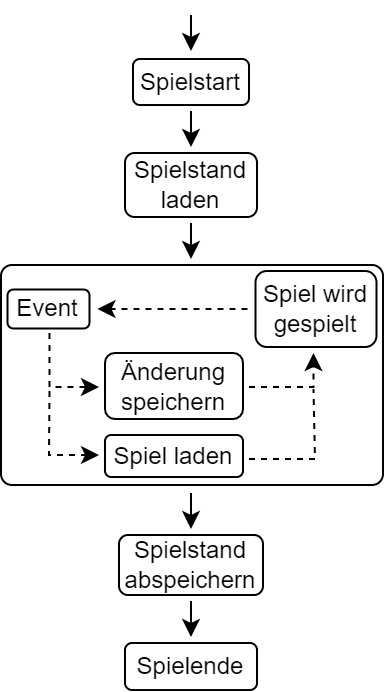
\includegraphics[scale=0.5]{images/Speichersystem.png}
    \caption{Phasen eines allgemeinen Speicher- und Ladesystems}
    \label{fig:speicherphasen}
\end{figure}

\begin{itemize}
    \item Spielstand laden kann alles auf einmal oder nur teile geladen werden (siehe mehr im Kapitel \ref{sect:ladesysteme})
    \item Je nach Speichersystem müssen hier teilweise noch die gespeicherten Daten überarbeitet werden
    \item Je nach Speichersystem können die Events die in "Änderung speichern" behandelt werden in zwei Kategorien unterteilt werden:
    \begin{enumerate}
        \item Ein Spielobjekt wurde hinzugefügt/geändert
        \item Ein Spielobjekt wurde gelöscht
    \end{enumerate}
    \item Spiel laden nach Events, wenn der Spieler sich z.B. in neuen Bereichen der Map befindet, die noch geladen werden müssen (mehr dazu in \ref{sect:ladesysteme})
    \item Spielstand am Ende abspeichern, vor Spielende optional (je nach Speichersystem notwendig)
\end{itemize}

Chunk-basiertes Speichersystem, welches Daten in Chunks verpackt:
\begin{figure}[H]
    \centering
    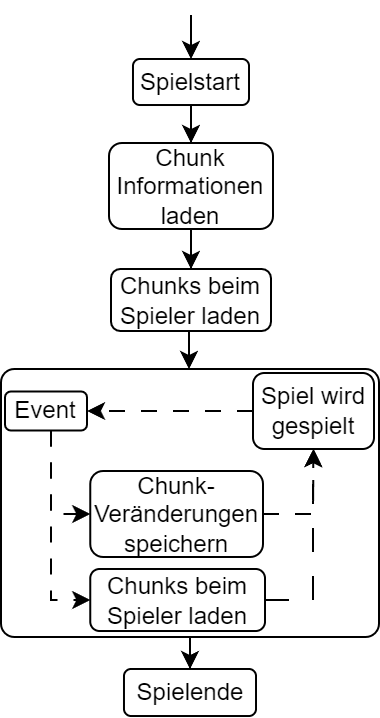
\includegraphics[scale=0.5]{images/Speichersys1.png}
    \caption{Chunk-basiertes System}
    \label{fig:chunkbasedsystem}
\end{figure}

Wobei ein Chunk aus folgenden Variablen besteht:
\begin{figure}[H]
    \centering
    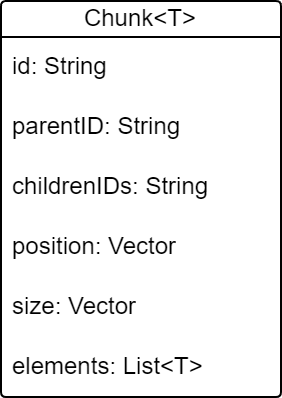
\includegraphics[scale=0.5]{images/Chunk.png}
    \caption{Chunk Klasse}
    \label{fig:chunkClass}
\end{figure}

ParentID und ChildrenIDs sind optional.

\begin{itemize}
    \item Chunks haben Position und Größe
    \item Dynamische oder statische Chunk Größe (Entweder alle Chunks feste Größe, oder sie passen sich an Datenmenge an)
    \item Chunks speichern Objekte, die in deren Bereich sind
    \item Objekte eines Chunks erst dann laden, wenn nötig (Z.B. Spieler in der Nähe); sowohl am Anfang, als auch während des Spieles
    \item Chunk Veränderungen speichern bei statischer Chunkgröße:
    \begin{itemize}
        \item Daten zu Chunkinhalt komplett neu speichern bei update/added/removed Objekt Event
    \end{itemize}
    \item Chunk Veränderungen speichern bei dynamischer Chunkgröße:
    \begin{itemize}
        \item Daten zu Chunkinhalt komplett neu speichern bei update/added Objekt Event 
        \item Chunkgröße bei added/removed Objekt Event überprüfen
        \item Chunkdaten komplett vom Speicher löschen, wenn dieser im Spiel gelöscht wird (beim Joinen mit benachbarten Chunks)
        \item Chunkdaten updaten und hinzufügen, wenn ein Chunk auf weiter Child-Chunks gesplitted wird
    \end{itemize}
\end{itemize}
    \chapter{Speicherarten}\label{ch:speicherarten}

Kapitel Optimierungen vielleicht eher in Kapitel 2, aber vielleicht gibt es 
Optimierung in der Datenbank

\section{Datenbanken}
NoSQL (JSON), SQL, usw. ausprobieren und Laufzeiten messen für die verschiedenen Algorithmen 
und Vor- und Nachteile (in Bezug auf Speichersystem für Videospiele) aufzählen. 

\subsection{NoSQL}
\subsubsection{JSON}

\subsection{SQL}

\section{Optimierungen}
-Komprimierung der Daten (Zip; aufpassen auf Betriebssysteme, vielleicht sieht das bei Mac/Linux anders aus als Windows)

    \chapter{Game Engines}\label{ch:gameengines}
Eine \textit{Game Engine} ist ein komplexes Software-Framework, das für die Erstellung, Entwicklung und Bereitstellung interaktiver digitaler Anwendungen konzipiert ist, vor allem für Videospiele, aber auch für Simulationen, Architekturvisualisierungen und vieles mehr. Dabei ist das Hauptziel einer Game Engine, eine Abstraktion der allgemeinen Videospielfunktionen anzubieten, damit Code und Spielkomponente in verschiedenen Projekten wiederverwendet werden können. Die Funktionen einer modernen Game Engine können eine Rendering-Engine für 2D- oder 3D-Grafiken, Handhabung von Inputs, Physik-Engine, Animationen, Speichermanagement und Prozess-Threading sein. Bei vielen modernen Game Engines verwenden Entwickler höhere Programmiersprachen, wie Java, C++ und C\#, zum Entwickeln der Skripte für die Spiele. Außerdem werden immer mehr Plattformen angeboten, für welche die Spiele entwickelt werden können, sei es für Desktop-Umgebungen, Mobilgeräte oder Konsolen.\cite{andrade2015game}

In diesem Kapitel werden drei Game Engines genauer betrachtet. Es wird die populäre Game Engine Unity\cite{vsmid2017comparison}, die von Epic Games veröffentlichte Unreal Engine und die neuere Godot Engine angeschaut. Alle Game Engines bieten eine Vielzahl an Möglichkeiten an, den Spielstand von einem Spieler abzuspeichern und zu laden. Teilweise gibt es auch bereits fertige Speicher- und Ladesysteme, die als Entwickler verwendet werden können.
%--------------------------------------------------------------------------



%--------------------------------------------------------------------------
\section{Unity}
\textit{Unity} ist eine leistungsstarke und vielseitige Echtzeit-3D-Entwicklungsplattform zum Entwickeln von Videospielen und Filmen. Sie wurde 2005 von Unity Technologies entwickelt und wurde durch die intuitive Benutzeroberfläche schnell zu der meist-verwendeten Game Engine der Welt. Unity bietet für Spieleentwickler eine breite Auswahl an Systemen an, für das Programmieren von 2D- und 3D-Spielen, Simulationen oder interaktiven Anwendungen. Es ist möglich Unity für Mobilspiele, verschiedenen Betriebssysteme, wie Windows, MacOS oder Linux, oder Spiele für Konsolen zu entwickeln. Programmiert wird bei Unity hauptsächlich mit der Programmiersprache C\#.\cite{unityUnityEngine}\cite{vsmid2017comparison}

In diesem Kapitel wird eine Vielzahl an Möglichkeiten angeschaut, welche Unity anbietet, um Speicher- und Ladesysteme für das Speichern des Spielstandes aufzustellen. Als erstes wird Unitys PlayerPrefs-Klasse angeschaut. Danach werden verschiedene Arten aufgezählt, Objekte von Unity in \ac{json} zu serialisieren und wann welche Strategie sinnvoll ist. Anschließend werden die .NET-Klassen BinaryFormatter, StreamWriter und StreamReader betrachtet. Beim BinaryFormatter werden die Probleme beim Serialisieren und Deserialisieren von Daten erläutert und es werden Alternativen vorgestellt. Abschließend wird das kostenpflichtige Paket Easy Save aus dem Asset Store angeschaut, welches einfach und effizient ein komplettes Speicher- und Ladesystem für Spiele implementieren kann.



\subsection{PlayerPrefs}
Bei Speicher- und Ladesystemen bietet Unity für Entwickler wenige eingebaute Funktionen. Jedoch gibt es die PlayerPrefs, welche eine einfache Art ist Daten zu speichern, aber ist dabei auch sehr limitiert. PlayerPrefs, was für Player Preferences steht, ist eigentlich zum Speichern von Konfigurationen, wie die Auflösung oder Lautstärke des Spieles gedacht. Jedoch lassen sich damit jede Art von Informationen speichern. Das Speichern wird mit Funktionen der PlayerPrefs-Klasse gemacht, wobei nur die Datentypen string, float und integer unterstützt werden. Über einen Schlüssel lässt sich dann ein Schlüsselwert dieser Datentypen festlegen oder es kann dieser erhalten werden. Die Werte der PlayerPrefs-Klasse werden mit der klasseninternen Save-Funktion gespeichert. Diese kann während der Laufzeit im Code aufgerufen werden und wird automatisch bei der Terminierung des Spieles aufgerufen.\cite{unityPlayerPrefsSave} Je nach Betriebssystem werden die PlayerPrefs in einem unterschiedlichen Dateiformat abgespeichert, die Daten werden aber nicht verschlüsselt.\cite{unityPlayerPrefs}

Allgemein wird davon abgeraten, Unitys PlayerPrefs-System für das Speichern des Spielstandes zu verwenden.\cite{unityPersistentData}\cite{logrocketPlayerPrefs}\cite{gamedevbeginnerPlayerPrefs} Zum Einen werden die Daten eines Spieles alle am selben Ort abgespeichert. Wenn es aber in dem Spiel verschiedene Spielstände geben soll, gibt es bereits Probleme mit diesem Ansatz. Eine mögliche Lösung von diesem Problem wäre es, dass jeder Spielstand eine Identifikationsnummer bekommt, welche dann an jedem Schlüssel hinzugefügt wird.\cite{logrocketPlayerPrefs} Die ganzen Identifikationsnummern müssen aber auch gespeichert werden, wo auch schon das nächste Problem mit PlayerPrefs auftritt. Es gibt wenige verfügbare Datentypen, die verwendet werden können. Wenn zum Beispiel eine Liste der Identifikationsnummern aller Spielstände gespeichert werden soll, kann dies nicht ohne größeren Aufwand gemacht werden.\cite{logrocketPlayerPrefs} Über den string-Datentyp lassen sich jedoch \ac{json}-Strings speichern, wodurch wieder mehr Datentypen, wie Listen und andere Gruppierungen von Daten, möglich sind. Wie auch schon erwähnt ist die PlayerPrefs-Klasse zum Speichern von Konfigurationen gedacht, nicht zum Speichern des Spielstandes. Bei Windows werden die PlayerPrefs in der Registry abgespeichert. Die Registry, oder auch Windows-Registrierungsdatenbank genannt, ist zum Speichern von Konfigurationen des Systems und von Anwendungen.\cite{logrocketPlayerPrefs} Bei größeren Datenmengen könnte dieses System sehr langsam werden.\cite{gamedevbeginnerPlayerPrefs}


\subsection{JSON}
Falls viele Daten gespeichert werden sollen und der Aufwand für den Entwickler gering gehalten werden soll, ist \ac{json} eine gute Alternative zu den PlayerPrefs. Auch hier bietet Unity ein Tool namens \textit{JsonUtility} an, welches die C\#-Objekte über Data Binding serialisieren kann. JsonUtility hat zwar einige Einschränkungen, ist dafür aber die schnellste Art, Objekte in \ac{json} zu serialisieren. Eine Einschränkung von JsonUtility ist, dass es einige Typen gibt, die nicht unterstützt werden, wie Dictionary<>, multidimensionale oder Jagged\footnote{Jagged Arrays sind Arrays, dessen Elemente Arrays aus verschiedener Größe sind.\cite{microsoftVerzweigteArrays}} Arrays. Diese lassen sich nicht mit JsonUtility serialisieren. In dem Listing \ref{lst:jsonUtilityExp} werden die drei Funktionen, die JsonUtility anbietet, demonstriert. Von der Zeile 1 bis 7 wird eine Spieler-Klasse definiert, welche dann in einer anderen Klasse, wie ab der Zeile 11 zu sehen ist, verwendet wird. Diese muss mit dem Attribut "Serializable" gekennzeichnet werden, damit diese auch serialisierbar ist. Alle Variablen, die in dieser Klasse public oder mit "[SerializeField]" gekennzeichnet werden, werden beim Serialisierungsprozess betrachtet. Als erstes werden drei Spieler-Objekte definiert, welche in den Zeilen 15 bis 18 zu \ac{json}-Strings serialisiert werden. In der Zeile 16 ist zu sehen, wie einer der \ac{json}-Strings aussieht. Der Spieler mit dem Namen "Joe" wird dann in den letzten zwei Zeilen zweimal überschrieben. Einmal mit den Werten der Spielerin "Alice" und einmal mit den Werten des Spielers "Tom".\cite{unityJsonUtility}\cite{unitySerializationRules} 

\begin{listing}[htp]
    \begin{minted}{csharp} 
        [Serializable]
        public class Player
        {
            public int level;
            public float health;
            public string name;
        }

        ...
        
        Player joe = new Player() { level = 1, health = 75.2f, name = "Joe" };
        Player alice = new Player() { level = 3, health = 100.0f, name = "Alice" };
        Player tom = new Player() { level = 2, health = 1.0f, name = "Tom" };

        string joeJson = JsonUtility.ToJson(joe);
        //  {"level":1,"health":75.2,"name":"Joe"}
        string aliceJson = JsonUtility.ToJson(alice);
        string tomJson = JsonUtility.ToJson(tom);

        joe = JsonUtility.FromJson<Player>(aliceJson);
        JsonUtility.FromJsonOverwrite(tomJson, joe);
    \end{minted}
    \caption{Serialisieren und Deserialisieren mit JsonUtility}
    \label{lst:jsonUtilityExp}
\end{listing}

Eine populäre Alternative zu JsonUtility ist die \textit{Newtonsoft.JSON}-Bibliothek, auch bekannt als \textit{Json.NET}. Sie wird sehr häufig bei C\#-Projekten verwendet, da sie einfach zu verwenden ist und das Umwandeln zwischen .NET-Objekten und \ac{json} in schnellen Laufzeiten bewältigen kann.\cite{newtonsoftJsonNETNewtonsoft} Der Vorteil gegenüber JsonUtility ist, dass alle nicht serialisierbaren Klassen von JsonUtility mit Json.NET serialisierbar sind. Es ist beispielsweise möglich, ein Dictionary<> zu serialisieren\cite{newtonsoftSerializeDictionary}\cite{newtonsoftDeserializeDictionary} oder jegliche Arten von Arrays. Json.NET wird auch seit der Unity Version 2018.4\footnote{Die Unity Version 2018.4 wurde 2019 veröffentlicht.\cite{unityDownloadArchive}} als Paket unterstützt.\cite{NewtonsoftJsonUnitySupport} Beim Serialisieren von Objekten werden auch bei Json.NET alle Variablen, die public sind, serialisiert. Um beim Serialisieren weniger Daten entstehen zu lassen, bietet Json.NET einige Funktionen an, wie zum Beispiel das Attribut "[JsonIgnore]", mit dem sich Variablen beim Serialisierungsprozess ignorieren lassen, oder die NullValueHandling Einstellung, mit der eingestellt werden kann, ob null-Werte gespeichert werden sollen. Dadurch, dass Json.NET viele Einstellungen anbietet, bei denen der komplette Serialisierungsprozess anpassbar ist, lassen sich die Laufzeiten für Projekte stark optimieren.\cite{newtonsoftReducingSerialized}\cite{newtonsoftPerformanceTips}

Eine weitere .NET-Bibliothek, die verwendet werden kann, ist \textit{LitJSON}. Auch diese ermöglicht es, .NET-Objekte in \ac{json} und umgekehrt zu konvertieren.\cite{litjsonLitJSONDocumentation} LitJSON bietet zwar weniger Funktionen als Json.NET an, aber es ist mithilfe des JsonReader und JsonWriter möglich, über die LitJSON Streaming API zu serialisieren und somit eine eigene Serialisierung der Klassen zu konstruieren.\cite{litjsonLitJSONReaders} Es gibt auch eine Bibliothek, wo LitJSON angepasst wurde, damit die .NET-Bibliothek auch für Unity verwendet werden kann.\cite{githubGitHubMervillUnityLitJson}

Wenn für das Unity-Projekt mit \ac{json} die Spielstände gespeichert werden sollen, stellt sich die Frage, welche Serialisierungs-Klasse oder -Bibliothek sich besser eignet. Wie in der Abbildung \ref{fig:unityJsonPerformance} zu sehen, ist JsonUtility die schnellste Art, Objekte in \ac{json} umzuwandeln und umgekehrt. Die schnellen Laufzeiten von JsonUtility haben auch den Preis, dass die Klasse etwas eingeschränkt ist und einfach gehalten wurde. Sobald es komplexere Datenstrukturen gibt, ist das Arbeiten mit JsonUtility eine große Herausforderung. Da kann sich der Entwickler dann doch für Json.NET oder LitJSON entscheiden, da diese mehr Datentypen unterstützten. Wenn es wichtig ist, dass das Programm schnell serialisiert werden soll, dann ist LitJSON die bessere Wahl zum Arbeiten mit \ac{json}. Falls das Deserialisieren möglichst schnell laufen soll, ist Json.NET geeigneter.

\begin{figure}[htp]
    \centering
    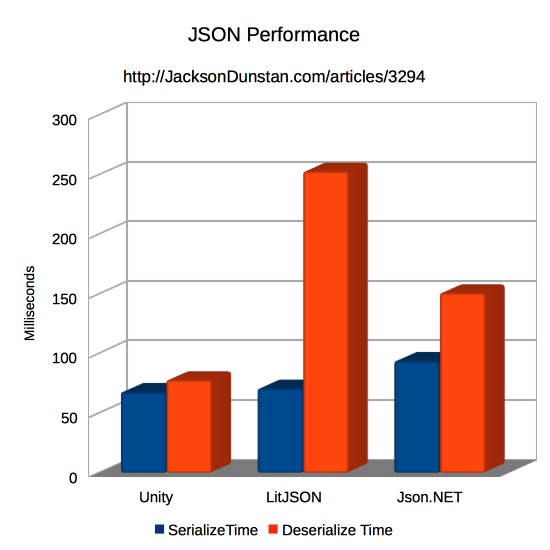
\includegraphics[width=0.6\textwidth]{images/UnityJsonPerformance.png}
    \caption{Laufzeiten der unterschiedlichen \ac{json}-Bibliotheken für Unity bei einer Datenmenge von 101 Bytes \cite{jacksondunstanJacksonDunstancomJSON}}
    \label{fig:unityJsonPerformance}
\end{figure}



\subsection{BinaryFormatter}\label{ssec:binaryFormatter}
Die .NET-Klasse \textit{BinaryFormatter} ist eine Möglichkeit, eine binäre Serialisierung der Daten durchzuführen. Sie verwandelt .NET-Objekte in eine Liste von Bytes um und umgekehrt. In dem Listing \ref{lst:binaryFormatterExp} ist zu sehen, wie der BinaryFormatter verwendet werden kann. Dabei werden die Player-Klasse und die Spieler aus dem Listing \ref{lst:jsonUtilityExp} benutzt. In der Zeile 2 wird der Spieler namens "Joe" in der Datei "joeFile" in binärer Form abgespeichert. In der Zeile 3 wird das Objekt namens "tom" mit den Werten aus der "joeFile"-Datei neu gesetzt. Dabei werden die Daten aus "joeFile" wieder deserialisiert.\cite{microsoftBinaryFormatterClass} 

\begin{listing}[htp]
    \begin{minted}{csharp} 
        BinaryFormatter formatter = new BinaryFormatter();
        formatter.Serialize(joeFile,joe);
        tom = (Player) formatter.Deserialize(joeFile);
    \end{minted}
    \caption{Serialisieren und Deserialisieren der Objekte aus \ref{lst:jsonUtilityExp} mit dem BinaryFormatter}
    \label{lst:binaryFormatterExp}
\end{listing}

Allgemein wird jedoch von dem Verwenden des BinaryFormatters abgeraten. Die Gefahr von Sicherheitsrisiken beim Deserialisieren ist groß. Ein Angreifer könnte den abgespeicherten Binärcode so verändern, dass dieser Code im Kontext des Zielprozesses ausführen wird. Je nach Anwendungstyp können solche Angriffe auch zu einem DoS-Angriff\footnote{Bei einem Denial of Service Angriff wird das Zielsystem mit etlichen Anfragen überflutet, was zu einer starken Verlangsamung, bis hin zu einem Zusammenbruch des Systems führen kann.\cite{bundDoSDDoSAttacken}} oder Veröffentlichung von Informationen führen.\cite{microsoftDeserializationRisks}

Eine sicherere Alternative zum BinaryFormatter sind die .NET-Klassen \textit{BinaryReader} und \textit{BinaryWriter}. Diese bieten Funktionalitäten, zum Schreiben von primitiven Datentypen in Binärcode und zum Umwandeln von Binärcode in primitive Datentypen an. Mit dieser Methode ist es zwar aufwendiger, die Daten zu speichern und zu laden, aber dafür sicherer als der BinaryFormatter.\cite{microsoftBinaryReaderClass}\cite{microsoftBinaryWriterClass} 

Ansonsten, wenn die Datenstrukturen komplexer werden, kann der Protocol Buffer aus \ref{sssec:binSerialisierung} verwendet werden. Als Entwickler kann entweder direkt der Protocol Buffer verwendet werden, da dieser auch C\# unterstützt \cite{protobufLanguageGuide}, oder es kann mit Tools gearbeitet werden, die das Kompilieren der Proto-Dateien in Unity übernehmen.\cite{githubProtobufUnity}



\subsection{StreamWriter und StreamReader}
Eine weitere Alternative zu \ac{json} und dem binären Serialisieren der Daten mit Unity sind die .NET-Klassen StreamWriter und StreamReader. Mit dem StreamWriter lassen sich Zeilen in Dateien schreiben und mit dem StreamReader lassen sich diese dann lesen.\cite{microsoftStreamWriterKlasse}\cite{microsoftStreamReaderKlasse} Als Entwickler kann dann entschieden werden, ob Formate wie \ac{json}, Binärcode oder XML verwendet werden, oder ob zum Speichern der Daten ein eigenes Format konzipiert werden soll. Zum Beispiel können einfache Datenstrukturen, wie eine Liste von Identifikationsnummern, Zeile für Zeile in einer eigenen Datei gespeichert werden. Es kann zu Komplikationen kommen, wenn das Format zum Speichern der Daten geändert wird. Die alten Daten müssten dann alle in das neue Format übersetzt werden.



\subsection{Easy Save}
Falls ein Entwickler Zeit sparen will und etwas Budget für das Projekt bereitstellt, kann das \textit{Easy Save} Paket vom Unity Asset Store in Betracht gezogen werden. Dieses Tool bietet ein komplettes Speicher- und Ladesystem für Unity-Projekte an, um eine einfache und effiziente Verwaltung der Daten zu ermöglichen.\cite{unityEasySave} In dem Listing \ref{lst:easySaveExp} ist zu sehen, wie ein Wert in das Speichersystem mit aufgenommen werden kann, indem das Level des Spielers gespeichert und geladen wird. ES3 ist die Klasse von Easy Save und wie zu sehen ist, werden die Daten mit einem Schlüssel-Wert-System gespeichert, ähnlich wie bei einem Dictionary.\cite{moodkieGettingStarted} Easy Save unterstützt viele Datentypen, wie Struct, Array, Dictionary, HashSet oder ganze Components\footnote{Die Basis-Klasse in Unity die an den Spielobjekten (GameObject-Klasse) hinzugefügt werden kann.\cite{unityComponent}}.\cite{moodkieSupportedTypes} Falls ein Datentyp nicht von Easy Save unterstützt wird, kann mit den ES3Types ganz einfach neue Datentypen zu dem System hinzugefügt werden.\cite{moodkieChoosingWhat} Es ist auch möglich, die gespeicherten Daten zu verschlüsseln oder zu komprimieren.\cite{moodkieGettingStarted} Vorausgesetzt, die Daten sollen automatisch gespeichert werden, kann die "Auto Save"-Funktion von Easy Save verwendet werden.\cite{moodkieAutoSave} Um eine bessere Leistung aus dem Speicher- und Ladesystem herauszuholen, kann mit Easy Save direkt eine Datei zum Speichern der Daten im Cache erstellt werden. Daten, die dann dort gespeichert werden, können während der Laufzeit schneller geladen werden.\cite{moodkieImprovingPerformance} Außerdem lassen sich Strings und Bytes direkt in den Speicherdateien schreiben und lesen.\cite{moodkieSavingLoading} 

\begin{listing}[htp]
    \begin{minted}{csharp} 
        int playerLevel = 1;
        ES3.Save("playerLevel", playerLevel);
        ... 
        if(ES3.KeyExists("playerLevel")) playerLevel = ES3.Load<int>("playerLevel")
    \end{minted}
    \caption{Speichern und Laden eines Integers mit Easy Save}
    \label{lst:easySaveExp}
\end{listing}



\subsection{Strategie für Unity}
Wie zu sehen ist, gibt es verschiedene Herangehensweisen für das Speichern und Laden des Spielstandes mit Unity. Welche Strategie ist für Unity am sinnvollsten? Kurz gesagt gibt es kein System, das in jedem Szenario das vorteilhafteste ist. Welche Strategie verwendet werden sollte, hängt von der Situation ab. 

Wenn Schnelligkeit und Kompaktheit der Daten die oberste Priorität sind, ist die binäre Serialisierung die beste Wahl (siehe \ref{fig:protobufTime} und \ref{fig:protobufBrowser}). Der Protocol Buffer wäre dabei die einfachste Art, dies umzusetzen, vor allem wenn die Datenstrukturen komplexer sind. Es gibt bereits viele Entwickler, die den Protocol Buffer in ihrem Unity-Projekt verwenden, da die C\#-Unterstützung bereits vorhanden ist. 

Falls der Entwickler oder Spieler die gespeicherten Daten lesen und bearbeiten können sollten, ist die Serialisierung zu \ac{json} sinnvoller. Wenn das Spiel zum Beispiel \acp{mod} haben soll, die von individuellen Spielern und Entwicklern erstellt werden können, dann sind Formate wie \ac{json} einfacher zu verstehen. Falls Geschwindigkeit das Wichtigste an dem Projekt ist, ist das JsonUtility-Tool von Unity die beste Wahl (siehe \ref{fig:unityJsonPerformance}). Hier muss jedoch für manche Datenstrukturen eine Serialisierung zu \ac{json} entwickelt werden, was bei komplexen Datenstrukturen sehr aufwendig sein kann. Falls die Zeit lieber gespart werden soll, ist Json.NET oder LitJSON eine gute Alternative. Beide sind im Vergleich zu JsonUtility zwar etwas langsamer, jedoch fällt dies erst bei sehr großen Datenmengen auf. Dadurch, dass beide aber mehr Datenstrukturen unterstützten, kann ein Entwickler bei der Serialisierung mit dieses Tools viel Zeit sparen. Im Durchschnitt ist Json.NET etwas schneller als LitJSON (siehe \ref{fig:unityJsonPerformance}), wenn jedoch schnelle Serialisierungszeiten wichtig sind, dann sollte LitJSON verwendet werden. Dies wäre zum Beispiel vorteilhaft, wenn es viele Serialisierungsprozesse gibt und nur am Anfang des Spieles die Daten deserialisiert werden.  

Ansonsten, wenn der Entwickler möglichst wenig Zeit für das Entwickeln des Speicherns und Ladens des Spielstandes brauchen möchte, ist das Easy Save Paket eine gute Alternative. Dieses bietet auch viele Optimierungsmöglichkeiten an, um das System effizienter laufen zu lassen. Für Unity gibt es auch kostenfreie Speicher- und Ladesysteme, wie zum Beispiel das Component-Save-System\footnote{https://github.com/AlexMeesters/Component-Save-System} von Alex Meesters. 
%--------------------------------------------------------------------------



%--------------------------------------------------------------------------
\section{Unreal Engine}
\textit{Unreal Engine} ist eine von Epic Games entwickelte Spiele-Engine, die von vielen größeren Entwicklungsteams verwendet wird. Unreal Engine ist aber auch bei einzelnen Entwicklern sehr beliebt, da es kostenlos und anfängerfreundlich ist. Bei realistischen Grafiken, Vegetation und Erstellung von Terrain für Videospiele liegt Unreal Engine auf Platz eins unter den Game Engines.\cite{vsmid2017comparison} Diese Entwicklungsplattform ist vor allem für größere Projekte gemacht, obwohl es auch Unterstützung für iOS und Android gibt. Mithilfe der Blueprints lassen sich Spiele visueller erstellen. Blueprints sind Graphen, die aus Blöcken bestehen, die zusammen verbunden sind. Jeder Block hat dabei eine Funktion, die ausgeführt wird. Bei der Unreal Engine wird hauptsächlich mit der Programmiersprache C++ oder Blueprints gearbeitet.\cite{vsmid2017comparison}

In diesem Abschnitt werden verschiedene Strategien betrachtet, die Unreal Engine zum Speichern und Laden von Spielständen anbietet. Als erstes wird die Unreal Engine "SaveGame"-Klasse angeschaut, welche über C++-Code und Blueprints ermöglicht, ein vollständiges System zum Speichern und Laden von Daten aufzustellen. Anschließend wird betrachtet, welche Möglichkeiten Unreal Engine anbietet, Daten in \ac{json} zu serialisieren und später diese zu deserialisieren. Zum Schluss wird ein Plugin für Unreal Engine 4 vorgestellt, mit dem in wenigen Schritten ein vollständiges Speicher- und Ladesystem aufgestellt werden kann. 



\subsection{SaveGame}
Seit Unreal Engine 4 wird die \textit{SaveGame}-Klasse bereitgestellt. Sie bietet dem Entwickler ein fertiges Speicher- und Ladesystem für den Spielstand. Dies kann entweder in einem Blueprint oder mit C++-Code eingestellt werden. Die Daten werden dann in einer ".sav"-Datei\footnote{SAV-Dateien sind Textdateien, die mehrere Kodierungsstandards wie ASCII, EBCDIC und Unicode unterstützten \cite{filextSavDatei}} abgespeichert.\cite{unrealengineSavingLoading}

Ein Beispiel für ein Blueprint zum Speichern der Spieldaten mit der SaveGame-Klasse ist in der Abbildung \ref{fig:unrealSaveGameBluePrintSave} zu sehen. Beim Erstellen dieses Blueprints muss als Elternklasse die SaveGame-Klasse ausgewählt werden. In diesem Beispiel heißt die Klasse "MySaveGame". In dieser Klasse können Variablen angelegt werden, die dann gespeichert und geladen werden sollen. Der Knoten "Create Save Game Object" in dem Blueprint erstellt ein neues Objekt der SaveGame-Klasse. In diesem Knoten muss dann "MySaveGame" als SaveGame-Klasse ausgewählt werden, damit mit den erstellten Variablen dieser Klasse gearbeitet werden kann. Mithilfe von "Set"-Knoten können die Werte der einzelnen Variablen in der eigenen SaveGame-Klasse gesetzt werden. Zum Speichern der Werte wird der "Save Game to Slot"-Knoten verwendet. Wenn das Speichern asynchron ablaufen soll, wird stattdessen der "Async Save Game to Slot"-Knoten verwendet, welcher von Epic Games empfohlen wird, wenn viele Daten gespeichert werden müssen. Dieser braucht als Eingabe ein SaveGame-Objekt, einen Slot-Namen und einen Benutzer-Index. Dabei wird der Slot-Name für den Namen der Speicherdatei und der Benutzer-Index als Benutzer-Identifikationsnummer verwendet. In dem Beispiel aus \ref{fig:unrealSaveGameBluePrintSave} werden für die Eingaben dieser die Standardwerte übergeben. Als Ausgabe-Pin gibt es einmal das SaveGame-Objekt der Eingabe und ob das Speichern erfolgreich war.\cite{unrealengineSavingLoading}

\begin{figure}[htp]
    \centering
    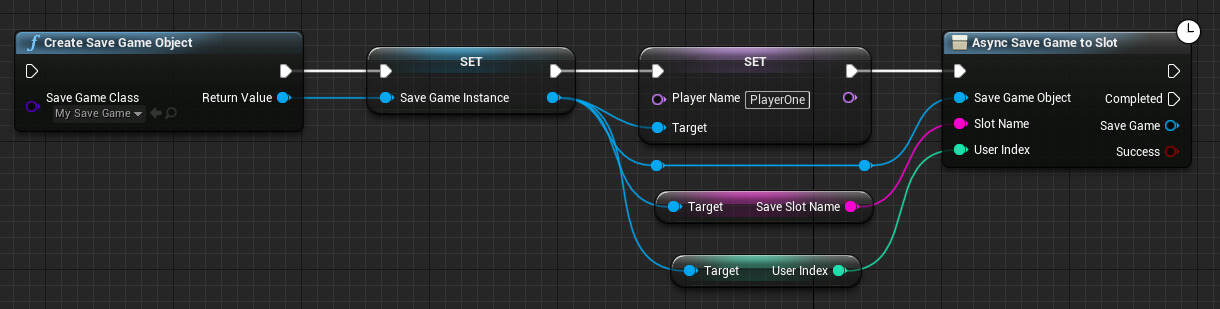
\includegraphics[width=1\textwidth]{images/SaveGameBP.png}
    \caption{Blueprint zum Speichern des Spielstandes mit der SaveGame-Klasse \cite{unrealengineSavingLoading}}
    \label{fig:unrealSaveGameBluePrintSave}
\end{figure}

Wie das Laden der Spieldaten mit der SaveGame-Klasse funktioniert, ist in dem Blueprint der Abbildung \ref{fig:unrealSaveGameBluePrintLoad} zu sehen. Zu Beginn wird der "Load Game from Slot"-Knoten gebraucht, um die Daten zu laden. Falls viele Daten geladen werden, oder es während der Ladezeit ein Lade-Bildschirm geben soll, wird auch hier von Epic Games der "Async Load Game from Slot"-Knoten empfohlen, der das Gleiche wie der "Load Game from Slot"-Knoten macht, aber asynchron arbeitet. Als Eingabe braucht dieser Knoten den Slot-Namen und den Benutzer-Index. Der Ausgabewert muss dann zur eigenen SaveGame-Klasse gecasted werden. Bei einem asynchronen Laden sollte zuerst mithilfe des "Is Valid"-Knotens überprüft werden, ob die Daten alle erfolgreich geladen wurden. Nach dem Cast zu der eigenen SaveGame-Klasse kann auf die Variablen dieser Klasse zugegriffen werden.\cite{unrealengineSavingLoading}

\begin{figure}[htp]
    \centering
    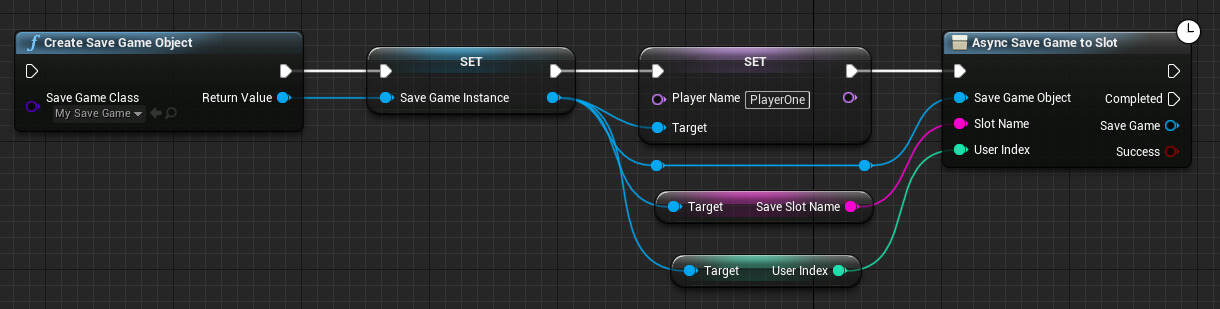
\includegraphics[width=1\textwidth]{images/SaveGameBP.png}
    \caption{Blueprint zum Laden des Spielstandes mit der SaveGame-Klasse \cite{unrealengineSavingLoading}}
    \label{fig:unrealSaveGameBluePrintLoad}
\end{figure}

Falls dieses Speicher- und Ladesystem in C++-Code geschrieben werden soll, muss die Header-Datei "Kismet/GameplayStatics.h" zu der eigenen SaveGame-Klasse hinzugefügt werden und diese muss dann als Kind-Klasse von der USaveGame-Klasse deklariert werden. In der eigenen SaveGame-Klasse können dann die zu speichernden Variablen, der Slot-Name und der Benutzer-Index definiert werden. Mithilfe der Funktion SaveGameToSlot oder AsyncSaveGameToSlot und LoadGameFromSlot oder AsyncLoadGameFromSlot aus der Klasse UGameplayStatics können die Daten synchron oder asynchron gespeichert und geladen werden.\cite{unrealengineSavingLoading}



\subsection{JSON}
Auch bei Unreal Engine ist es möglich, die Spieldaten im \ac{json}-Format abzuspeichern. Bei den Blueprints ist der Entwickler etwas eingeschränkt, da es erst seit Unreal Engine 5 Blueprints zum Arbeiten mit \ac{json} gibt und die Anzahl der Funktionen noch gering ist. Es gibt Knoten für Blueprints, bei denen ein C++-Struct zu einem \ac{json}-String umgewandelt wird, oder Knoten, bei denen bestimmte Schlüsselwerte von \ac{json}-Objekten zurückgegeben werden. Außerdem gibt es Knoten, die \ac{json}-Objekte aus Dateien speichern und laden können.\cite{unrealengineJsonBlueprint}

Mehr Möglichkeiten gibt es beim direkten Arbeiten mit C++, um zu \ac{json} zu serialisieren. Dafür gibt es zum Beispiel bei Unreal Engine eine \textit{FJsonSerializer}-Klasse.\cite{unrealengineFJsonSerializer} Zum Speichern der \ac{json}-Daten als C++-Objekt kann die FJsonObject-Klasse verwendet werden.\cite{unrealengineFJsonObject} Zum Serialisieren und Deserialisieren wird dann der FJsonSerializer benutzt.\cite{unrealengineFJsonSerializer} In dem Listing \ref{lst:unrealFJsonSerializer} ist zu sehen, wie diese Klassen verwendet werden können. In den ersten vier Zeilen wird ein neues \ac{json}-Objekt erstellt, mit Schlüssel und Schlüsselwerten wie in dem Listing \ref{lst:jsonUtilityExp}. Danach wird in der Zeile 8 dieses \ac{json}-Objekt zu einem \ac{json}-String konvertiert und in dem Objekt "JsonString" gespeichert. In der Zeile 12 wird dieser String wieder deserialisiert und in einem \ac{json}-Objekt namens "JsonObject" gespeichert. Falls das Deserialisieren erfolgreich abläuft, ist die Kondition aus der Zeile 12 wahr und der Code in der Zeile 14 kann ausgeführt werden.\cite{wraiythUsingJson1}\cite{wraiythUsingJson2}

\begin{listing}[htp]
    \begin{minted}[breaklines,frame=single]{cpp}
        TSharedPtr JoeJsonObject = MakeShareable(new FJsonObject);
        JoeJsonObject->SetNumberField("level", 1);
        JoeJsonObject->SetNumberField("health", 75.2f);
        JoeJsonObject->SetStringField("name", "Joe");
        
        FString JsonString;
        TSharedRef<TJsonWriter<>> Writer = TJsonWriterFactory<>::Create(&JsonString);
        FJsonSerializer::Serialize(JoeJsonObject.ToSharedRef(), Writer);   
        
        TSharedPtr JsonObject;
        TSharedRef<TJsonReader<>> Reader = TJsonReaderFactory<>::Create(JsonString);
        if(FJsonSerializer::Deserialize(Reader, JsonObject)) 
        {
           ...
        }
    \end{minted}
    \caption{Serialisieren und Deserialisieren mit FJsonSerializer in Unreal Engine \cite{wraiythUsingJson1}\cite{wraiythUsingJson2}}
    \label{lst:unrealFJsonSerializer}
\end{listing}



\subsection{Save Extension}
Falls ein Entwickler ein fertiges Speicher- und Ladesystem sucht, welches er in sein Spiel integrieren möchte, dann ist \textit{Save Extension} geeignet. Dieses Plugin wurde für Unreal Engine 4 gemacht und bietet eine Vielzahl an Funktionen an, die sowohl in C++-Code als auch als Blueprint implementiert werden können.\cite{unrealengineSaveExtension}

Die ersten Schritte zum Aufstellen des Speicher- und Ladesystems mit der Save Extension über ein Blueprint sind in der Abbildung \ref{fig:unrealSaveExtensionBlueprint} zu sehen. Die zwei Knoten "Save Slot to Id" und "Load Slot from Id" werden verwendet, um Daten aus einem bestimmten Slot zu speichern und zu laden. Jeder Slot kann eine bestimmte Spielwelt von einem Spieler sein und wird in einer eigenen Datei gespeichert.\cite{piperiftPiperiftSaveSlot} Um einen bestimmten Slot auszuwählen, gibt es die Eingabe "Slot Id", in der die Slot-Nummer eingegeben werden kann. Beim Speichern kann auch ausgewählt werden, ob der alte Spielstand eines Slots überschrieben werden soll, falls einer existiert. Zum Auslösen des Speicherns oder Ladens gibt es einige Möglichkeiten. In der Abbildung \ref{fig:unrealSaveExtensionBlueprint} zum Beispiel wird das Speichern des Spielstandes dadurch ausgelöst, dass die Taste K gedrückt wurde. Zum Laden muss in diesem Beispiel die Taste L gedrückt werden. Alternativ unterstüzt das Save Extension-Plugin auch ein Auto-Save und Auto-Load. Beim Auto-Save wird automatisch der aktuelle Slot gespeichert und beim Auto-Load wird immer der letzte aktive Slot geladen. Ein Slot wird als aktiv markiert, wenn er geladen wird.\cite{piperiftPiperiftSaveSlot}\cite{piperiftPiperiftSaveBlueprint} 

\begin{figure}[htp]
    \centering
    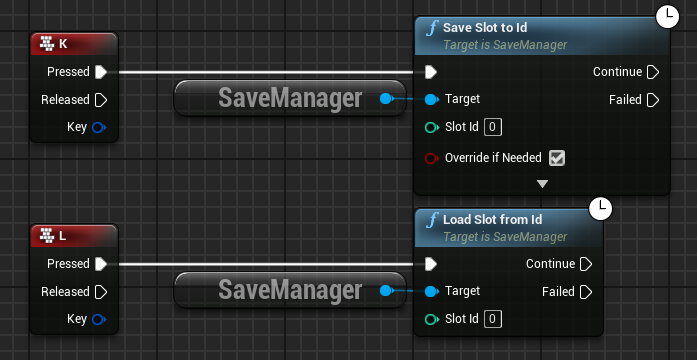
\includegraphics[width=0.8\textwidth]{images/SaveExtension_load_save_blueprint.png}
    \caption{Blueprint zum Laden der Daten mit dem Save Extension-Plugin \cite{piperiftPiperiftSaveBlueprint}}
    \label{fig:unrealSaveExtensionBlueprint}
\end{figure}

Nach dieser Einrichtung werden noch keine Actor\footnote{Actors sind bei Unreal Engine alle Spielobjekte, die in der Spielwelt geladen werden.\cite{unrealengineActors}}-Klassen oder Components\footnote{Components werden an Actors angehängt und beeinflussen, wie diese sich verhalten.\cite{unrealengineActors}} gespeichert. Über das \textit{SavePreset} Blueprint lassen sich Actors und Component-Klassen zum Speicher- und Ladesystem hinzufügen. Um dann Variablen eines Actors oder Components abzuspeichern, muss für jede zu speichernde Variable die "SaveGame"-Eigenschaften angeklickt werden. Komprimierung der Daten ist bei der Save Extension auch möglich. Dies kann bei dem SavePreset eingestellt werden.

Um zu vermeiden, dass zu viele Daten geladen werden, werden Slots in zwei Bereiche unterteilt und gespeichert. Es gibt einmal die Slot Info, die leichtgewichtete Daten über die Spielwelt speichert. Diese enthält zum Beispiel das Level des Spielers, seinen Spielername oder in welchem Bereich der Spielwelt sich der Spieler bei dem Spielstand befindet. Der Rest wird im "Slot Data"-Bereich gespeichert. Hier sind alle Informationen der serialisierten Actors und Components der Spielwelt eines Slots. Diese Unterteilung ist praktisch, wenn wenige Slot-Informationen benötigt werden, aber diese nicht komplett geladen werden sollen. Falls zum Beispiel ein Menü erstellt wird, wo ausgewählt werden kann, mit welcher Spielwelt weitergespielt werden soll, kann hier bei jeder Spielwelt ein paar Informationen über diese beschrieben werden, ohne alle Slots komplett zu laden.\cite{piperiftPiperiftSaveSlot}

Eine weitere Funktion, die die Effizienz des Speicherns enorm verbessern kann, ist die Möglichkeit, asynchron zu arbeiten. Bei dem Save Extension-Plugin gibt es einmal die Multithreaded oder Frame-splitted Serialisierung, bei der die zu serialisierenden Daten auf alle verfügbaren CPU-Threads oder auf mehreren Frames verteilt und dort einzeln serialisiert werden. Außerdem gibt es noch Multithreaded-Dateien, die asynchron im Hintergrund der Anwendung komprimiert, gespeichert und geladen werden.\cite{piperiftPiperiftSaveMultithreaded}

Der Speicherprozess besteht aus den folgenden Schritten: Als Erstes wird der alte Spielstand gelöscht und es wird die Funktion OnSaveBegan aufgerufen, um weiterzugeben, dass der Speicherprozess begonnen hat. Dann werden der Thumbnail des aktuellen Spieles und die Spielstatistiken abgespeichert und anschließend wird die Spielwelt serialisiert. Zum Schluss wird die Funktion OnSaveFinished aufgerufen, um weiterzugeben, dass der Speicherprozess beendet wurde. In der Abbildung \ref{fig:piperiftSaveProcess} ist der vollständige Speicherprozess zu sehen. Gestrichelte Kanten bedeuten, dass hier mehrere Prozesse parallel laufen können.\cite{piperiftSaveProcess}

\begin{figure}[htp]
    \centering
    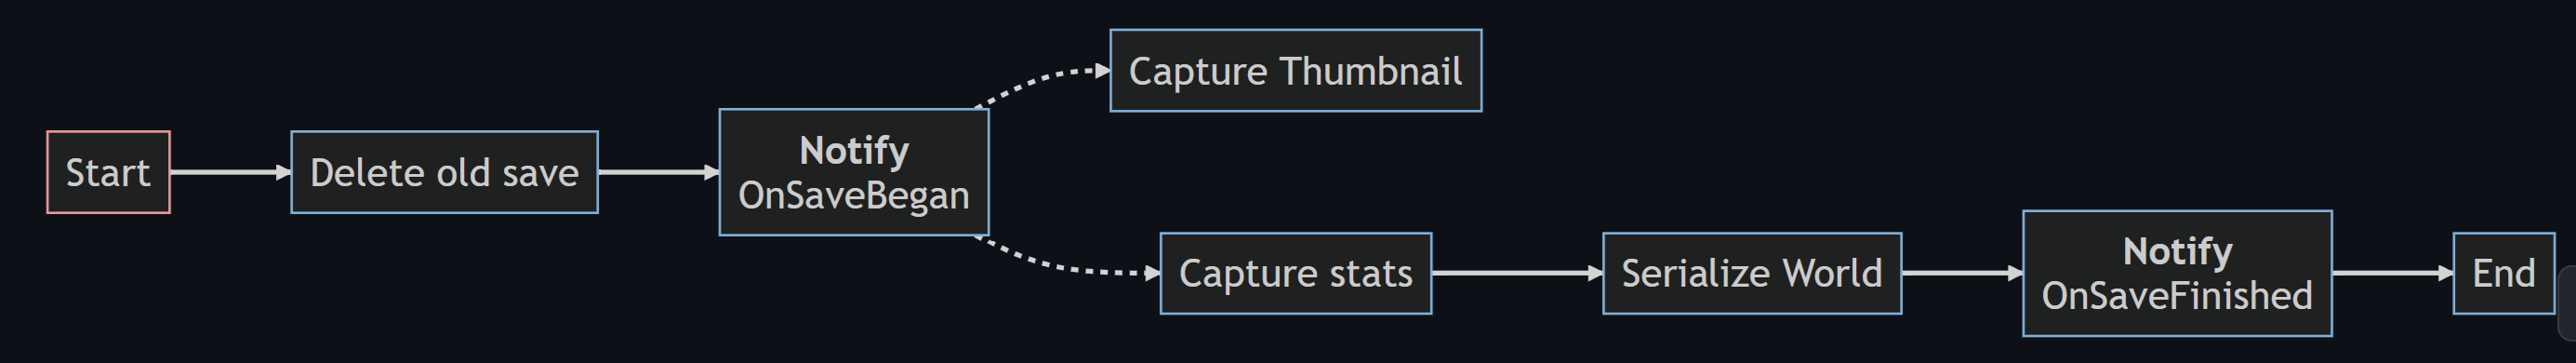
\includegraphics[width=1\textwidth]{images/piperift_save_process.png}
    \caption{Speicherprozess des Save Extension-Plugins \cite{piperiftSaveProcess}}
    \label{fig:piperiftSaveProcess}
\end{figure}

Der Ladeprozess ist etwas komplexer. Als erstes wird die Funktion OnLoadBegan aufgerufen, um den Start des Ladeprozesses weiterzugeben. Danach werden alle Maps und Daten geladen und anschließend werden die Filter der einzelnen Level und generelle Filter vorbereitet, damit überprüft werden kann, welcher Actor in welchem Level geladen werden muss und wie dieser deserialisiert werden soll. Hiernach werden die einzelnen Levels vorbereitet und die Welt wird deserialisiert. Beim Vorbereiten der Levels werden gespeicherte Actors wiederhergestellt und nicht mehr existierende endgültig gelöscht. Beim Deserialisieren der Welt werden alle Level abgearbeitet und deren Actors und Components deserialisiert. Zum Schluss wird die Funktion OnLoadFinished aufgerufen, um weiterzugeben, dass der Ladeprozess terminiert hat. In der Abbildung \ref{fig:piperiftLoadProcess} ist der vollständige Ladeprozess zu sehen.\cite{piperiftLoadProcess}

\begin{figure}[htp]
    \centering
    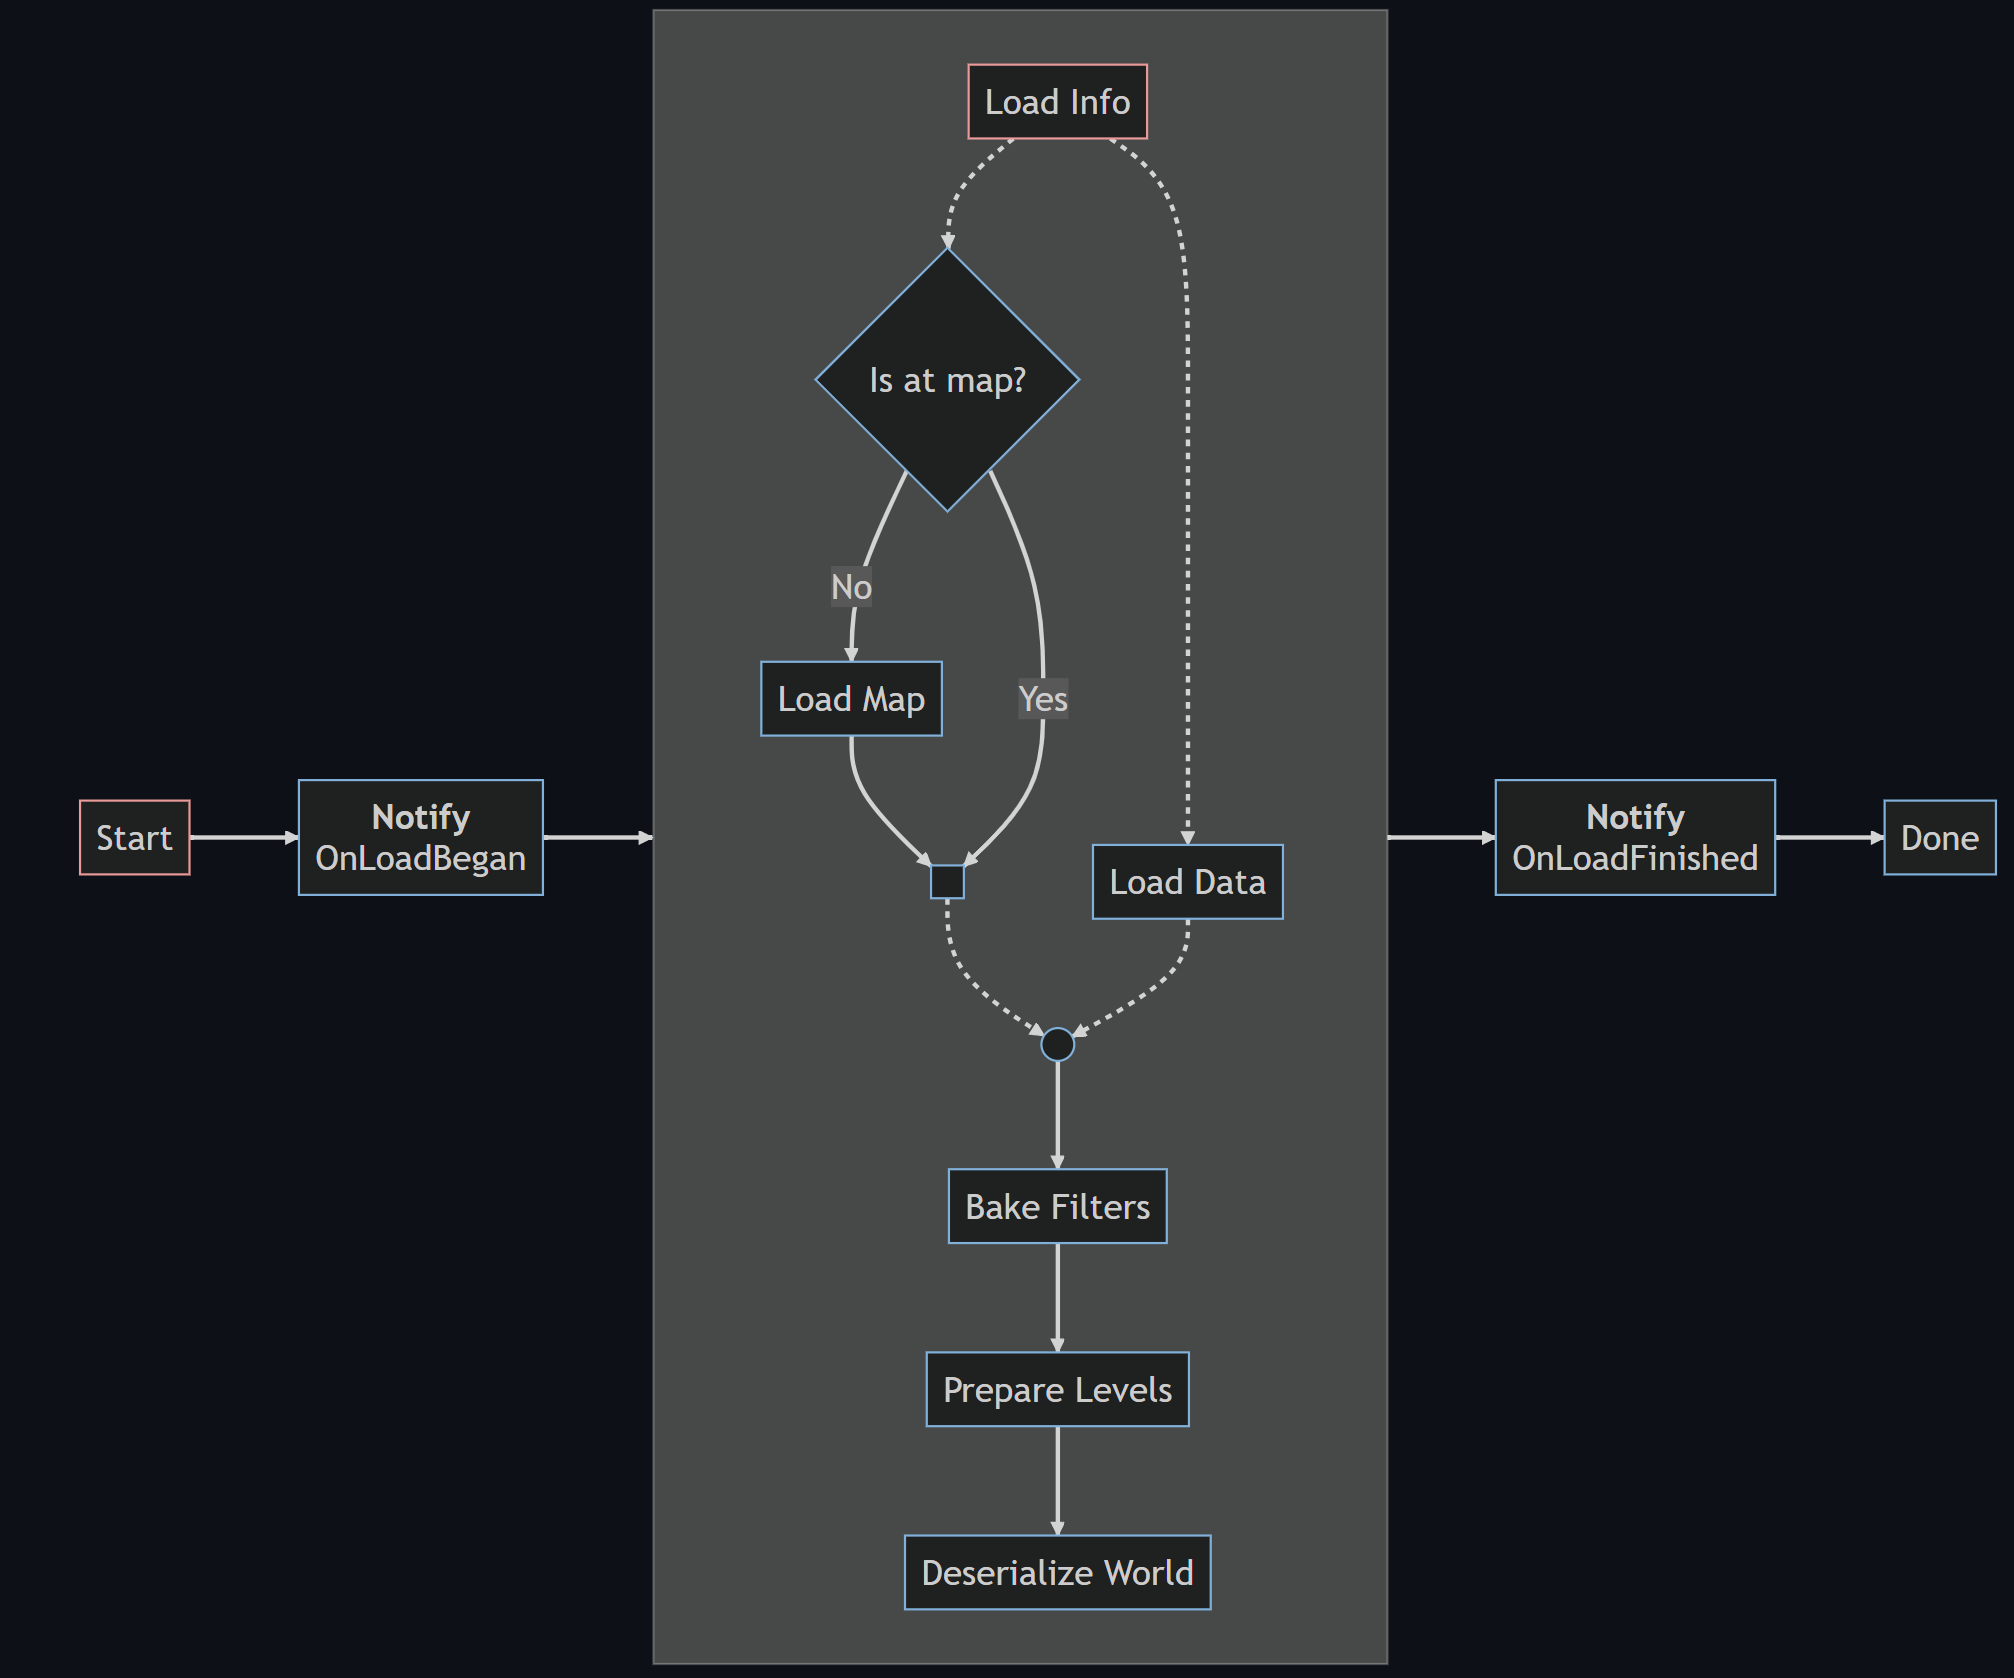
\includegraphics[width=0.8\textwidth]{images/piperift_load_process.png}
    \caption{Ladeprozess des Save Extension-Plugins \cite{piperiftLoadProcess}}
    \label{fig:piperiftLoadProcess}
\end{figure}



\subsection{Strategie für Unreal Engine}
Auch bei Unreal Engine gibt es keine beste Lösung für das Speichern und Laden von Spielständen. Bei den von Unreal Engine bereitgestellten Tools eignet sich am besten die SaveGame-Klasse. Diese wird von Epic Games empfohlen, wenn ein Speicher- und Ladesystem aufgebaut werden muss. Die Serialisierung zu \ac{json} über die Blueprints, die schon in Unreal Engine eingebaut sind, scheint umständlich zu sein, da sie wenige Funktionen anbietet. 

Falls das System ohne Problem auf mehr Daten erweitert werden soll, wird das Arbeiten mit Blueprints ein großer Aufwand. Bei vielen Daten, die gespeichert werden sollen, wird es schnell unübersichtlich mit der graphischen Oberfläche der Blueprints und den vielen Verbindungen unter den Knoten. Außerdem wird bei fortgeschrittenen Entwicklern empfohlen, C++ zu verwenden, da damit effizientere Algorithmen als mit den Blueprints entwickelt werden können.\cite{epicgamesComparingBlueprints} Als Alternative zu der Blueprint-Strategie kann die FJsonSerializer- oder SaveGame-Klasse von Unreal Engine verwendet werden. Welche Option geeigneter ist, hängt auch von den Präferenzen des Entwicklers ab. Falls die Daten im \ac{json}-Format gespeichert werden müssen, ist die FJsonSerializer-Klasse angebrachter. Ansonsten kann auch hier die von Epic Games empfohlene SaveGame-Klasse verwendet werden, um mit C++-Code die Daten zu speichern.

Auch bei Unreal Engine kann ein fertiges Speicher- und Ladesystem verwendet werden, falls der Entwickler möglichst viel Zeit sparen möchte. Die Save Extension ist eine gute Alternative zu den von Epic Games bereitgestellten Tools. Sie ist kostenfrei und bietet einige Möglichkeiten an, den Speicher- und Ladeprozess zu beschleunigen. 
%--------------------------------------------------------------------------



%--------------------------------------------------------------------------
\section{Godot}
Godot Engine ist ein open-source und kostenfreies Game Engine, welches von einer Gemeinschaft von unabhängigen Entwicklern erstellt wurde. Es wurde 2014 veröffentlicht und wird hauptsächlich für kleinere Spiele verwendet, da es im Vergleich zu anderen Game Engines weniger Funktionen bereitstellt. Im Vergleich zu Unity und Unreal Engine verwendet Godot keinen komponentenbasierten Ansatz, sondern hat verschiedene Klassen von Objekten, die Nodes genannt werden. Diese werden in einer Hierarchie in der Spiel-Szene angeordnet und jedem Node kann ein Skript angehängt werden, um dessen Verhalten anzupassen. Statt bereits existierende Programmiersprachen zu verwenden, wurde für Godot eine eigene Programmiersprache entwickelt, namens GDScript, welche viele Ähnlichkeiten zu Python besitzt. Alternativ können aber auch C\# und C++ verwendet werden. Mit der Godot Engine können 2D- und 3D-Spiele für Desktop-Plattformen, Mobilgeräte und das Web entwickelt werden.\cite{salmela2022game}

Zu Beginn von diesem Abschnitt werden zwei Möglichkeiten betrachtet, die von Godot Engine angeboten werden, um Spielobjekte zu serialisieren und deserialisieren. Einmal wird das Arbeiten mit \ac{json} betrachtet und danach die binäre Serialisierung. Zum Schluss wird noch ein Godot-Plugin vorgestellt, welches ein fertiges Speicher- und Ladesystem für Entwickler anbietet. 



\subsection{JSON}
Da die Programmiersprache GDScript Dictionaries unterstützt, ist es sinnvoll, mit \ac{json} zu arbeiten, da diese im GDScript bereits eine sehr \ac{json}-ähnliche Struktur besitzen. Um ein Speicher- und Ladesystem mit Godot Engine im \ac{json}-Format aufzustellen, sollten zu Beginn erst einmal alle Objekte, die gespeichert werden sollen, markiert werden. Jedes Objekt kann zu einer Gruppe hinzugefügt werden. Gruppen sind Ansammlungen von Objekten mit einem bestimmten Namen, wobei jedes Objekt auch mehreren Gruppen zugehören kann. Danach muss zu allen Objekten, die gespeichert werden sollen, eine Funktion hinzugefügt werden, die das Objekt zu einem \ac{json}-Objekt umwandelt. Wie so eine Funktion aussehen kann, ist in dem Listing \ref{lst:godotJsonToJsonFunc} zu sehen. Alle wichtigen Variablen eines Objektes werden in ein Dictionary gespeichert und danach mithilfe der "\ac{json}"-Hilfsklasse zu einem \ac{json}-String umgewandelt. Diese Klasse hat aber auch Einschränkungen, was alles in \ac{json} umgewandelt werden kann. Zum Beispiel können Vektoren, wie der "position"-Vektor eines Objektes, nicht direkt in \ac{json} umgewandelt werden. Deshalb muss die Position über eine x- und y-Variable gespeichert werden, statt direkt den "position"-Vektor zu speichern.\cite{godotengineSavingGames}

\begin{listing}[htp]
    \begin{minted}[breaklines,frame=single,tabsize=2]{python}
        func to_json():
          var object_data = {
            "filename" : get_scene_file_path(),
            "parent" : get_parent().get_path(),
            "x" : position.x, 
            "y" : position.y,
            "level": level,
            "health": health,
            "name": name
          }

          return JSON.stringify(object_data)
    \end{minted}
    \caption{Konvertierung der zu speichernden Klassendaten zu \ac{json} in Godot \cite{godotengineSavingGames}}
    \label{lst:godotJsonToJsonFunc}
\end{listing}

Die "to\_json"-Funktion kann zum Speichern aller Objektzustände verwendet werden. In dem Code \ref{lst:godotJsonSave} ist zu sehen, wie eine Speicherfunktion aussehen könnte. Dabei wird als erstes eine Datei definiert, in der die Daten gespeichert werden sollen. Danach werden alle Objekte aus der "Save"-Gruppe geholt und über diese Menge wird iteriert. Wenn ein Objekt gespeichert werden soll, muss es zu dieser Gruppe hinzugefügt werden. Für jedes Objekt dieser Gruppe wird erst einmal geschaut, ob dieses Objekt aus einer Datei instanziiert wurde und ob in diesem Objekt die "to\_json"-Funktion enthalten ist. Nodes bei Godot haben immer die Variable "scene\_file\_path", welche als String speichert, aus welcher Datei das Objekt instanziiert wurde. Alle Kind-Nodes dieses Objektes haben bei dieser Variable einen leeren String.\cite{godotengineNode} Diese Nodes sollen beim Speichern übersprungen werden. Bei den restlichen Objekten wird die "to\_json"-Funktion aufgerufen und der \ac{json}-String, der zurückgegeben wird, wird in die Speicherdatei geschrieben.\cite{godotengineSavingGames} Falls sich ein Dateiname der Objekte verändern sollte, weil der Entwickler diese zum Beispiel geändert hat, müssen alle Spielstände angepasst werden, da ansonsten die Datei der Objekte nicht gefunden werden kann.

\begin{listing}[htp]
    \begin{minted}[breaklines,frame=single]{python}
        func save_game():
          var save_game = FileAccess.open("user://savegame.save", FileAccess.WRITE)
          var save_nodes = get_tree().get_nodes_in_group("Save")
          for node in save_nodes:
            if node.scene_file_path.is_empty() || !node.has_method("to_json"): 
              continue 

            var json_string = node.call("to_json")
            save_game.store_line(json_string)
    \end{minted}
    \caption{Speichern aller JSON-Daten der Knoten aus der "Save"-Gruppe \cite{godotengineSavingGames}}
    \label{lst:godotJsonSave}
\end{listing}

Für das Laden der Daten müssen mehr Schritte durchgeführt werden. In dem Code \ref{lst:godotJsonLoad} ist zu sehen, wie ein Spiel in Godot über eine "load\_game"-Funktion geladen werden kann, abhängig von den letzten zwei GDScripts. Zu Beginn sollte überprüft werden, ob die Speicherdatei existiert. Wenn das der Fall ist, kann der Prozess fortgesetzt werden. Als nächstes wird geschaut, ob bereits Objekte der "Save"-Group existieren. Diese müssen gelöscht werden, weil sonst beim Laden Duplikate entstehen könnten. Danach kann begonnen werden, die Speicherdatei Zeile für Zeile abzulesen. Da die Objekte immer als einzeilige \ac{json}-Strings gespeichert werden, stellt jede Zeile in der Speicherdatei ein Objekt da. Dieses \ac{json}-Objekt wird dann über die "parse"-Funktion der \ac{json}-Hilfsklasse deserialisiert. Falls das Deserialisieren erfolgreich war, werden die Daten des Objektes an die "load\_node"-Funktion weitergegeben. Diese instanziiert das Objekt und setzt die Werte der gespeicherten Variablen.\cite{godotengineSavingGames}

\begin{listing}[htp]
    \begin{minted}[breaklines,frame=single]{python}
        func load_game():
          if not FileAccess.file_exists("user://savegame.save"):
            return

          var save_nodes = get_tree().get_nodes_in_group("Save")
          for i in save_nodes:
            i.queue_free()

          var save_game = FileAccess.open("user://savegame.save", FileAccess.READ)
          while save_game.get_position() < save_game.get_length():
            var json_string = save_game.get_line()
            var json = JSON.new()

            var parse_result = json.parse(json_string)
            if not parse_result == OK: continue

            load_node(json.get_data())

        func load_node(node_data):
          var new_object = load(node_data["filename"]).instantiate()
          get_node(node_data["parent"]).add_child(new_object)
          new_object.position = Vector2(node_data["x"], node_data["y"])

          for key in node_data.keys():
            if key == "filename" or key == "parent" or key == "x" or key == "y":
              continue
            new_object.set(i, node_data[i])
    \end{minted}
    \caption{Laden der in \ref{lst:godotJsonSave} gespeicherten Daten \cite{godotengineSavingGames}}
    \label{lst:godotJsonLoad}
\end{listing} 



\subsection{Binary Serialization}
Auch binäre Serialisierung wird von Godot unterstützt. Bei diesem Prozess werden die verschiedenen Datentypen zu einem Array von Bytes umgewandelt. Von Godot Engine werden 30 verschiedene Datentypen\cite{godotengineBinarySerialization} bereitgestellt, die im binären Format gespeichert werden können. Beim Serialisieren werden die Daten in Pakete verpackt. Ein Paket ist ein Datentyp mit seinem Wert. Die ersten vier Bytes eines Pakets beschreiben den Datentypen und werden zum Setzen von Flags verwendet. Jeder Datentyp ist als Zahl definiert, welche im Header binär geschrieben wird. Zum Beispiel ist der Datentyp "int" mit der Zahl 2 definiert und über Flags kann gespeichert werden, ob es ein 32-Bit- oder 64-Bit-Integer ist. Ab dem fünften Byte beginnt der Inhalt des Pakets. Dieser variiert von Datentyp zu Datentyp. Bei Strings zum Beispiel wird in den ersten vier Bytes des Inhalts definiert, wie lang die Zeichenkette ist, und erst nach diesen vier Bytes wird der String-Inhalt bestimmt. Bei solchen Datentypen ist die Größe des Paketinhalts variabel und nicht fest definiert.\cite{godotengineBinarySerialization}

Objekte können über Godots "var\_to\_bytes\_with\_objects"-Funktion binär serialisiert und mit der "bytes\_to\_var\_with\_objects"-Funktion wieder deserialisiert werden. Beim Deserialisieren muss jedoch beachtet werden, dass die Daten keinen Code beinhalten, der ausgeführt werden kann. Es sollten immer nur Daten von vertrauten Quellen deserialisiert werden, sonst können Probleme entstehen, die bei dem BinaryFormatter-Abschnitt \ref{ssec:binaryFormatter} genauer beschrieben wurden.\cite{godotengineGlobalScope}

Die binäre Serialisierung hat viele Vorteile gegenüber der \ac{json}-Serialisierung. Zum einen sind die Dateigrößen deutlich kompakter bei binären Daten, im Vergleich zu den gespeicherten \ac{json}-Strings. Außerdem unterstützt Godot viel mehr Datentypen, die binär, aber nicht zu \ac{json} serialisiert werden können. Bei eigenen Klassen braucht es auch eigene Logik zum Kodieren und Dekodieren dieser, um das Serialisieren zu \ac{json} zu ermöglichen. Bei binärer Serialisierung wird weniger eigene Logik benötigt.\cite{godotengineSavingGames}



\subsection{Thoth}
Falls ein fertiges Speicher- und Ladesystem gesucht wird, welches in das Projekt integriert werden soll, dann ist das Plugin \textit{Thoth} eine Alternative zu den eingebauten Godot Engine-Funktionen. Dieses System wurde so entwickelt, dass es für jede Art von Spiel verwendet werden kann und speichert den Spielzustand in einem Format, welches ähnlich zu \ac{json} ist.\cite{stupidratstudioGodotSaveLoad}

Um das System aufzustellen, muss das "Savestate"-Node von diesem Plugin hinzugefügt werden. Diese Node ist immer mit einer Speicherdatei verbunden und kann den Spielzustand zu einem beliebigen Zeitpunkt speichern. Im GDScript-Listing \ref{lst:godotThoth} ist zu sehen, wie das "Savestate"-Node verwendet werden kann. Als erstes wird in dem Array "serializable\_collections" definiert, welche Objekte serialisiert werden sollen. In dem Beispielcode werden alle Kinder-Nodes von dem "SaveObjects"-Node serialisiert. Bei jedem Objekt kann außerdem mit dem "serializable"-Array eingestellt werden, welche Variable gespeichert wird. In dem Objekt, zu dem der Code aus dem Listing \ref{lst:godotThothObject} gehört, werden zum Beispiel nur die Variablen "level", "health" und "name" gespeichert. Die Variable "effects" wird beim Serialisieren übersprungen. Zum Speichern und Laden müssen die Funktionen "save\_game" und "load\_game" aus dem Listing \ref{lst:godotThoth} aufgerufen werden. Bei der Speicherfunktion müssen als erstes die gespeicherten Daten geladen werden, da es möglich ist, dass noch Informationen der alten Spielstände gebraucht werden. Anschließend kann der aktuelle Spielzustand serialisiert und dann gespeichert werden. Bei der Ladefunktion wird als erstes der letzte Spielzustand geladen und danach deserialisiert.\cite{stupidratstudioGodotSaveLoad} 

\begin{listing}[htp]
    \begin{minted}[breaklines,frame=single]{python}
        extends Node2D

        const serializable_collections = [
          "SaveObjects"
        ]

        @onready var savestate = get_node("Savestate")

        func save_game():
          savestate.load_game_state()
          savestate.pack_game_state(self)  
          savestate.save_game_state()

        func load_game():
          savestate.load_game_state()
          savestate.unpack_game_state(self)
    \end{minted}
    \caption{Speichern und Laden des "SaveObjects"-Knoten mit Thoth \cite{stupidratstudioGodotSaveLoad}}
    \label{lst:godotThoth}
\end{listing} 

\begin{listing}[htp]
    \begin{minted}[breaklines,frame=single]{python}
        extends Node2D

        var level
        var health
        var name
        var effects

        const serializable = [
            "level",
            "health",
            "name"
        ]

        ...
    \end{minted}
    \caption{Thoth-Einstellung, welche Variablen einer Klasse serialisiert werden sollen \cite{stupidratstudioGodotSaveLoad}}
    \label{lst:godotThothObject}
\end{listing} 



\subsection{Strategie für Godot Engine}
Auch bei Godot gibt es keine Strategie, die vorteilhafter als alle andere ist beim Speichern und Laden des Spielstandes. Auch bei Godot ist dies abhängig vom Anwendungsfall. Falls das Speicher- und Ladesystem selber vom Entwickler komplett implementiert werden soll, eignet es sich, mit den eingebauten Tools von Godot Engine zu arbeiten. Hier hat die binäre Serialisierung auch mehr Vorteile. Sie ist schneller, die Daten sind kompakter und es werden deutlich mehr Datentypen unterstützt, wodurch der Entwickler weniger eigenen Code zum Serialisieren und Deserialisieren der Daten schreiben muss. Die einzigen Gründe, stattdessen die \ac{json}-Hilfsklasse zu verwenden, ist, dass die gespeicherten Daten im binären Format nicht von Menschen gelesen werden können und dass Veränderungen der Datenstruktur zu Problemen führen können. Wenn es dazu kommt, muss der Entwickler alle Daten selber auf die neue Datenstruktur anpassen. Falls die Lesbarkeit wichtig ist und sich die Datenstrukturen öfters verändern könnten, sollte mit \ac{json} gearbeitet werden.

Auch bei Godot hat ein Entwickler die Möglichkeit, Zeit durch das Verwenden eines fertigen Speicher- und Ladesystems zu sparen. Hier kann zum Beispiel Thoth verwendet werden, mit dem das System in wenigen Schritten implementiert werden kann. Da als Entwickler noch einige Zeilen Code geschrieben werden müssen, bei denen verschiedene Funktionen von Thoth aufgerufen werden, gibt es noch einige Möglichkeiten, das System anzupassen und gegebenenfalls zu optimieren.
    \chapter{Online}\label{ch:online}

Verschiedene Datenbanken und Algorithmen testen. 
Vielleicht einen neuen Algorithmus von Speichern und Laden mit Server verwenden (z.B. lokaler Zwischenspeicher verwenden, der Daten schonmal vorlädt)

    \chapter{Speichersysteme in Videospielen}\label{ch:videospiele}
In diesem Kapitel wird die Praxis von Speicher- und Ladesystemen betrachtet. Dabei werden verschiedene Spiele analysiert, um deren Prozesse des Speicherns und Ladens des Spielstandes genauer zu verstehen. Als erstes wird das Sandbox-Spiel Minecraft und danach das Strategiespiel Factorio angeschaut. 
%--------------------------------------------------------------------------


%--------------------------------------------------------------------------
\section{Minecraft}
Minecraft ist ein Sandbox-Spiel\footnote{Ein Sandbox-Spiel lässt Spieler frei entscheiden, was mit der Spielwelt gemacht werden soll. Es gibt keine feste Geschichte im Spiel, die verfolgt werden muss.\cite{ocio2009multi}}, welches von Mojang Studio entwwickelt wurde. Minecraft gilt unter den meistverkauften Videospiele aller Zeiten und kann auf eine Vielzahl von Plattformen gespielt werden.\cite{ignBestSellingVideo} Es wird in einer dreidimensionalen Welt, die aus Blöcken besteht, gespielt und es kann mit Entitäten interagiert werden. Es gibt verschiedene Spielmodi, wie zum Beispiel ein Überlebens- und Kreativmodus. Beim Überlebensmodus geht es hauptsächlich um das Überleben in der Spielwelt, jedoch kann der Spieler frei entscheiden, was er in der Spielwelt machen wird.\cite{minecraftWikiHome}

In diesem Abschnitt dieser Arbeit wird das Speicher- und Ladesystem von Minecraft genauer betrachtet. Als erstes wird ausgearbeitet, aus welchen Spielobjekten die Welt in Minecraft besteht, um herauszufinden, welche verschiedenen Daten gespeichert werden müssen. Danach wird geschaut, wie diese Daten bei Minecraft aufgeteilt werden, damit nur mit einer Teilmenge der ganzen Daten gearbeitet werden muss. Anschließend wird die Ordnerstruktur einer Spielwelt angeschaut, um ein tieferes Verständnis für die Aufteilung der Daten zu sichern. Danach werden die Formate der Dateien genauer betrachtet, um zu verstehen, wie die einzelnen Daten letztendlich in den Speicher geschrieben werden. Zum Schluss wird angeschaut, wie der Ablauf des gesamten Speicherprozess ist. Es wird erklärt, zu welchen Zeitpunkten der Spielzustand gesichert wird, damit möglichst wenig Daten der Spielwelt verloren gehen. Dabei wurde als Quelle ausschließlich die Minecraft Wiki\footnote{ Minecraft Wiki: \url{https://minecraft.fandom.com/wiki/Minecraft_Wiki}} verwendet, die von dem Minecraft Support empfohlen wurde (siehe die Abbildung \ref{fig:minecraftMail}). Sie dokumentiert alle Daten zu Minecraft, um ein tieferes Verständnis für das Spiel aufzubauen. Dadurch, dass es für Minecraft auch Modifikationen gibt, die von jeglichen Entwicklern geschrieben werden können, gibt es auch Möglichkeiten an den Quelltext von Minecraft zu kommen. Aus rechtlichen Gründen ist es jedoch leider nicht möglich, diesen freizugeben. Viele Inhalte der Minecraft Wiki wurden jedoch noch einmal geprüft, durch analysieren des Quellcodes.\todo{Autor mit einbeziehen; Ich habe den Quellcode mir angeschaut für die Arbeit}



\subsection{Daten}
Bevor sich das Speicher- und Ladesystem von Minecraft genauer angeschaut werden kann, ist es erstmal wichtig zu wissen, mit welchen Arten von Daten Minecraft arbeitet. Die Spielwelt in Minecraft besteht aus verschiedenen Blöcken, Entitäten\todo{Entitäten vs Entitys} und Items. 

\textit{Blöcke} werden in Minecraft nicht einzeln behandelt, sondern als Section, ein Bereich von 16x16x16-Block, gespeichert. Mehr zu dieser Aufteilung bei Minecraft gibt es im Abschnitt \ref{ssec:datenaufteilung}. Informationen, die zu so einem Block gehören, sind die Position, BlockID, Block Zustände und Informationen zum Licht. Die Position eines Blocks wird in der Reihenfolge y-, z- und x-Koordinate gespeichert, für bessere Komprimierung. Jeder Blocktyp hat eine eigene BlockID, die diesen Block genau identifiziert. Der Zustand eines Blocks wird für jede Section in einer Liste namens "BlockStates" abgespeichert. Informationen dessen Zustands können zum Beispiel sein, in welcher Himmelsrichtung der Block plaziert wurde, welche Rotation der Block hat und ob der Block am brennen ist. Welche Zustände ein Block haben kann, hängt auch von dem Blocktyp ab.\cite{minecraftBlockStates} Bei den Informationen zum Licht jedes Blocks gibt es für jede Section zwei Listen namens "BlockLight" und "SkyLight". "BlockLight" speichert wieviel Licht jeder Block ausstrahlt und "SkyLight" wieviel jeder Block an Licht abbekommt. Zusätlich gibt es noch sogenannte Block Entitys, die aber nichts mit den Entitäten des Spieles zu tun haben. Diese Speichern zusätliche Informationen zu einem Block, die in der "BlockStates"-Liste nicht gespeichert werden konnten.\cite{minecraftChunkFormat}
%Weitere Quelle: ChunkSerializer.java:write()

Eine Entität kann ein Spieler, ein Tier oder Monster sein. Die wichtigste Information einer Entität ist die Position, Geschwindigkeit und Rotation dieser. Des weiteren gibt es viele weitere Informationen zu einer Entität, wie die Luft die die Entität noch übrig hat zum Überleben, die Distanz die eine Entität schon gefallen ist oder wie lange eine Entität noch brennen wird.\cite{minecraftEntityFormat}
%Weitere Quelle: Entity.java:writeWithoutTypeID()

\textit{Items} bei Minecraft existieren im Inventar, in Kisten, in Item Frames oder in Armor Stands\todo{Englisch}. Wenn ein Spieler ein Item fallen lässt, dann werden diese als Entitäten in die Welt platziert und als solche gespeichert. Manche Items können in die Welt platziert werden und werden dann zu neuen Blöcken oder Entitäten. Jedes Item hat die Information "Count", "Slot", "id" und "tag". "Count" und "Slot" definieren, wieviele Items in welchem Inventarplatz liegen. Jedes Item hat dabei eine eigene Identifikationsnummer, mit der diese gespeichert werden. "tag" gibt noch zusätliche Informationen über ein Item, wie die Haltbarkeit oder ob ein Item unzerbrechlich ist.
\cite{minecraftPlayerdatFormat}
\cite{minecraftItem}

%Item werdeb z.B. in player.dat gespeichert



\subsection{Datenaufteilung} \label{ssec:datenaufteilung}
Die Spielwelt von Minecraft, mit seinen Blöcken, Entitäten und Items, werden nach einem Chunk-basiertem System aufgeteilt. Dieses System unterteilt die Welt in verschiedene Gruppierungen und Untergruppen, wobei die oberste Ebene die "Welt" selbst ist. In Minecraft bezeichnet eine "Welt" die Spielwelt, die von einem Spieler erstellt werden kann, und diese Welt wird wiederum in die drei Dimensionen "Overworld", "Nether" und "End" unterteilt.\cite{minecraftWorld}

Jede Dimension bekommt seine eigenen Dateien zum Speichern der Daten (siehe \ref{ssec:ordnerstruktur}). Eine Dimension kann theoretisch aus unendlich vielen Blöcken, Entitäten und Items bestehen. Sie wird dabei auf mehrere Regionen aufgeteilt. Eine Region besteht aus 1024 Chunks, wobei sie 32 Chunks breit und 32 Chunks lang ist.\cite{minecraftRegionFile} 

Was die Größe eines Chunks betrifft, so ist sie statisch und beträgt 16 Blöcke in der Länge, 16 Blöcke in der Breite und die Höhe variiert je nach der jeweiligen Höhe der Welt. Seit der Einführung der Minecraft Version 1.18 beträgt die maximale Höhe der Spielwelt 384 Blöcke.\cite{minecraftNewestJavaEdition}\cite{minecraftNewestBedrockEdition} Um diese Struktur weiter zu verfeinern, wird jeder Chunk in Sektionen unterteilt. Eine Sektion besteht aus insgesamt 4096 Blöcken, was bedeutet, dass sie 16 Blöcke in der Länge, Breite und Höhe umfasst.\cite{minecraftChunk}

%Chunk.java:sections



\subsection{Ordnerstruktur} \label{ssec:ordnerstruktur}
Ein Spieler kann in Minecraft verschiedene Spielwelten erstellen. Dabei bekommt jede dieser Spielwelten einen eigenen Ordner. Wie so ein Ordner aufgebaut ist, ist in der Ordnerstruktur aus \ref{lst:ordnerStrukturMinecraft} zu sehen. Die nicht-markierten Knoten entsprechen einem Ordner und die blauen Knoten sind Dateien in dem Speichersystem. In dem Ordner einer Welt sind noch ein paar weitere Ordner und Dateien, diese sind aber nicht relevant für diese Arbeit. Die erste Datei in dem Ordner, die "level.dat"-Datei, speichert globale Daten über die Spielwelt ab. In den Ordnern "playerdata", "stats" und "advancements" werden Spielerinformationen abgespeichert, über eine "<uuid>.dat"- oder "<uuid>.json"-Datei. Die "uuid" wird dabei durch die Identifikationsnummer des Spielers ersetzt. Wenn alleine gespielt wird, werden viele Spielerdaten auch in der "level.dat"-Datei gespeichert. In dem "stats"- und "advancements"-Ordner werden Statistiken und Fortschritte von jedem Spieler der Welt gespeichert. Falls eine Welt im Mehrspielermodus gespielt wird, enthalten die Dateien im "playerdata"-Ordner alle restlichen Informationen eines Spielers.\cite{minecraftPlayerdatFormat}. Die restlichen Ordner und Dateien speichern den Zustand der Spielwelt. Bei Minecraft gibt es zum Beispiel Weltkarten, die Teile der Spielwelt anzeigen können. Jede Weltkarte kann dabei unterschiedliche bereiche der Welt anzeigen, deshalb gibt es für jede Weltkarte eine "map\_<\#>.dat"-Datei, die den Zustand einer Weltkarte speichert. Die "villages.dat"-Datei speichert die Zustände aller Dörfer der Spielwelt, denn jedes Dorf ist ein komplexes System aus verschiedenen zufällig generierten Entitäten und Gebäuden. Da die Spielwelt von Minecraft aus verschiedenen Dimensionen, namens "Overworld", "Nether" und "End" besteht, werden manche Daten auf verschiedenen Ordnern verteilt. Im "DIM-1"-Ordner werden Informationen zu der "Nether"-Dimension gespeichert und der "DIM1"-Ordner ist für die "End"-Dimension. Die "entities"- und "region"-Ordner zum Beispiel enthalten Informationen über die Entitäten und Regionen der Spielwelt und sind auch in den Ordnern der verschiedenen Dimensionen zu finden. Alle Entitäten und Regionen, die in keinem "DIM-1"- oder "DIM1"-Ordner gespeichert wurden, gehören zu der "Overworld"-Dimension.\cite{minecraftFolderStruc}

\begin{listing}[htp]
    \dirtree{%
    .1 world.
        .2 \textcolor{blue}{level.dat}.
        .2 playerdata.
            .3 \textcolor{blue}{<uuid>.dat}.
        .2 stats.
            .3 \textcolor{blue}{<uuid>.json}.
        .2 advancements.
            .3 \textcolor{blue}{<uuid>.json}.
        .2 data.
            .3 \textcolor{blue}{idcounts.dat}.
            .3 \textcolor{blue}{map\_<\#>.dat}.
            .3 \textcolor{blue}{villages.dat}.
            .3 \dots.
        .2 entities.
        .2 region. 
            .3 \textcolor{blue}{r.<\#>.<\#>.mca}.
        .2 DIM-1.
            .3 entities.
            .3 region.
                .4 \textcolor{blue}{r.<\#>.<\#>.mca}.
            .3 \dots.
        .2 DIM1.
            .3 entities.
            .3 region.
                .4 \textcolor{blue}{r.<\#>.<\#>.mca}.
            .3 \dots.
        .2 \dots.
    } 
    \caption{Ordnerstruktur einer Spielwelt in Minecraft\cite{minecraftFolderStruc}}
    \label{lst:ordnerStrukturMinecraft}
\end{listing}



\subsection{Speicherformate}
Wie schon im vorherigen Abschnitt zu sehen ist, besitzt Minecraft eine handvoll verschiedener Formate, zum Speichern der Daten. Die Dateien haben Formate wie "dat", "mca" und "json". Natürlich existieren auch noch weitere Formate, wie PNG-Dateien für Texturen, da diese Dateien zu den statischen Daten dazugehören, werden diese nicht weiter betrachtet.   

Das DAT-Format wird für jegliche Arten von Informationen verwendet, sei es Video, Audio, PDF oder jede andere Art von Daten. Ein Programm kann DAT-Dateien erstellen und spezifisch für dieses Programm Daten abspeichern und lesen. Für andere Programme sind diese Daten nicht sonderlich hilfreich, da sie für ein spezifisches Programm erstellt wurden.\cite{adobeWhatDAT} Dieses Format wird zum Beispiel für die globalen Spielwelt Informationen in der "level.dat"-Datei oder für Spielerdaten in "<player>.dat"-Dateien, falls die Spielwelt auf einem Server gehosted wird (siehe \ref{ssec:ordnerstruktur}).\cite{minecraftPlayerdatFormat}\cite{minecraftFolderStruc}. 
Die Daten werden dabei im eigenen Format namens \ac{nbt} in diese Dateien geschrieben. Diese Format ist ähnlich zu dem \ac{json}-Format, denn die Daten werden auch hier im Schlüssel-Wert-Prinzip behandelt. Das \ac{nbt}-Format bietet eine Vielzahl an Datentypen, wie Byte, Boolean, verschiedene Zahlen Datentypen, String, List, Compound und Array. Der List-Datentyp ist zum Speichern von mehreren Werten, ohne Schlüssel. Compound ist eine geordnete Liste von Schlüssel-Wert-Paaren. Nachträglich werden in den meisten Fällen die \ac{nbt}-Dateien mit GZip komprimiert.
\cite{minecraftNBT}

\ac{mca} ist ein Dateiformat, zum Speichern von Chunk-Daten. Dabei wird in einer Datei eine Region, also eine Gebiet aus 32x32 Chunks, gespeichert. Jede Datei bekommt dann den Namen "r.<x>.<z>.mca", wobei x und z mit den x und z Koordinaten der Region ersetzt wird. Falls die Koordinaten einer Region gesucht werden, in der ein Chunk drin ist, müssen die Chunk-Koordinaten durch 32 geteilt und abgerundet werden. Eine \ac{mca}-Datei fängt mit einem 8 KiB Header an, der in zwei 4 KiB Blöcken unterteilt ist. Der erste Block beschreibt die Position der Chunks in der Region und der zweite Block speichert die Zeit, wann jeder Chunk zuletzt aktualisiert wurde. Nach dem Header werden alle Zustände der Chunks einer Region gespeichert. Dabei wird für jeden Chunk erst die Länge der Daten in Bytes angegeben, dann die Art der Komprimierung und anschließend die komprimierten Daten.\cite{minecraftRegionFile}\cite{minecraftAnvilFile} Auch in diesen Dateien werden die Daten im \ac{nbt}-Format in komprimiert Form gespeichert.\cite{minecraftNBT}

Das \ac{json}-Format wird für das Speichern von Texten und kleineren Daten verwendet. In Minecraft gibt es Bücher, Schilder und Labels, die der Spieler beschriften und mit Text füllen kann. Bücher zum Beispiel werden dann zwar im \ac{nbt}-Format in den Dateien zu den Spielerdaten gespeichert, aber die Seiten der Bücher werden als serialisierten \ac{json}-Text gespeichert.\cite{minecraftPlayerdatFormat} Die "advancements"- und "stats"-Ordner, die im Abschnitt \ref{ssec:ordnerstruktur} vorgestellt wurden, speichern die Fortschritte der einzelnen Spieler auch im \ac{json}-Format ab. Ansonsten wird \ac{json} hauptsächlich für statische Daten, wie das Verhalten von Entitäten, Blöcken und Items oder Anleitungen für das Bauen von Spielgegenständen.\cite{minecraftJSON}

%Siehe auch: RegionFileCache.java:loadFile(), SaveFormat.java:convertRegions()

\subsection{Speichervorgänge}
In den vorherigen Abschnitten wurde detailliert erörtert, welche Daten in Minecraft gespeichert werden und in welcher Form dies geschieht. Nun stellt sich die Frage nach dem genauen Ablauf des gesamten Speicherprozesses und den Zeitpunkten, zu denen die Daten gesichert werden.

Der Spielzustand einer Welt in Minecraft wird zu verschiedenen Zeitpunkten im Spielverlauf gesichert. Zunächst wird der initiale Zustand der Spielwelt gespeichert, wenn eine Welt neu generiert wird. Doch darüber hinaus erfolgen während das Spiel gespielt wird sowohl automatische als auch manuelle Speicherprozesse.\cite{minecraftSpielstandSpeicherung}

Manuelle Speicherungen finden statt, wenn der Spieler die Pause-Taste betätigt, die in Minecraft der "Esc"-Taste entspricht. Damit hat der Spieler die Möglichkeit, den aktuellen Zustand seiner Welt bewusst zu sichern.\cite{minecraftSpielstandSpeicherung} 

Automatische Speicherungen erfolgen hingegen in regelmäßigen Intervallen. Der Spielzustand wird alle fünf Minuten automatisch gesichert, um sicherzustellen, dass selbst bei unvorhergesehenen Ereignissen oder einem möglichen Absturz des Spiels nur minimaler Fortschritt verloren geht.\cite{minecraftSpielstandSpeicherung}

Chunks die zu weit weg von dem Spieler sind, werden bei Minecraft entladen, da es sehr viele Ressourcen brauchen würde, alle Chunks geladen zu lassen, auch wenn sie nicht aktiv verwendet werden. Bevor diese entladen werden, wird der Zustand des Chunks automatisch gesichert. Dies gewährleistet, dass keine relevanten Chunk-Informationen verloren gehen und diese bei Bedarf wiederhergestellt werden können.\cite{minecraftSpielstandSpeicherung}

Insgesamt sorgen diese verschiedenen Speichermechanismen in Minecraft dafür, dass der Spielverlauf zuverlässig und in verschiedenen Situationen gesichert wird, um den Verlust von Fortschritt auf ein Minimum zu reduzieren.

%Siehe auch: Minecraft.java:createWorld()
%Siehe auch: IntegratedServer.java:tick()



\subsection{Ladevorgänge}



\subsection{Fazit}
\begin{itemize}
    \item Chunk System mit fester Größe, da Limit an Elementen pro Chunk?
    \item Erwähnen, dass beim Spielen die Speicher- und die Ladezeiten nicht auffallen. Zu Beginn sind die Ladezeiten auch gering
\end{itemize}

\todo{Irgendwie zusammenfassen, welche Strategien Minecraft verwendet?}
%--------------------------------------------------------------------------



%--------------------------------------------------------------------------
\section{Factorio}
Factorio ist ein Spiel, wo das Hauptziel ist, eine Fabrik aufzubauen. Als Spieler muss man sich um Ressourcen kümmern, die abgebaut werden müssen, um damit neue Technologien zu erforschen und eine Infrastruktur aufzubauen. Um eine möglichst große Ausbeute für die eigene Fabrik zu erreichen, kann die Produktion automatisiert werden. Im Spiel gibt es außerdem noch Einheimische, die die Ausbeutung der Ressourcen anhalten wollen. Deshalb muss der Spieler zusätzlich zu dem Aufbauen seiner Fabrik diese auch noch vor den Einheimischen verteidigen, damit sie nicht kaputt geht. Factorio wurde von Wube Software in C++ geschrieben und 2016 auf der Plattform "Steam" veröffentlicht. Mittlerweile kann Factorio auf Windows, macOS, Linux und der Nintendo Switch gespielt werden.\cite{factorioMain}\cite{factorioPressFactorio}

In diesem Abschnitt wird das Speicher- und Ladesystem von Factorio genauer betrachtet. Als erstes wird analysiert, welche Daten das Spiel beinhaltet, und wie diese aufgeteilt werden. Anschließend werden die einzelnen Vorgänge des gesamten Speicher- und Ladeprozess angeschaut. Als Bezugsquelle für die Informationen zu dem System von Factorio wurde hauptsächlich mit den Quellen gearbeitet, die Wube Software empfohlen hat (siehe Abbildung \ref{fig:factorioMail}). Für ein tieferes Verständnis über die Prozesse des Spieles wurde außerdem die offiziellen Wiki von Factorio\footnote{Offizielle Wiki von Factorio: \url{https://wiki.factorio.com/} \cite{factorioPressFactorio}} verwendet.

\subsection{Daten}
Factorio benutzt Serialisierung und Deserialisierung, verwendet dabei aber verschiedene Formate zum Speichern der Daten. Welche verschiedenen Arten von Daten dann das Spiel hat, zeigt die Abbildung \ref{fig:factorioSaveStatistic}. Das Kreisdiagramm zeigt welche Arten von Daten wie viel Speicherplatz benötigen, bei 40 MB unkomprimierten Daten. Ungefähr 70\% des Speicherplatzes verbrauchen drei Kategorien der Spielobjekte, die Dekorations-Objekte, Tiles und Entitäten. Tiles sind Rechtecke, die das kleinste Stück in der Spielwelt darstellen. Die Tiles sind auch die Maßeinheiten für alle Gebiets- und Distanzabmessungen. Die Größe von Entitäten wird auch in Tiles angegeben. Zum Beispiel ist das "Rocket Silo", die größte Entität in dem Spiel, neun Tiles breit und lang. Die Spielwelt hat eine maximale Größe von zwei Millionen Tiles in der Breite und Länge, also vier Trillionen Tiles.\cite{factorioMapStructure} Die restlichen Daten sind aus der Blueprint Bibliothek, Physikalische Kräfte, Transportbänder, Oberfläche und Chunk Daten und weiteren kleineren Daten.\cite{factorioFridayFacts270} Die Blueprint Bibliothek ist ein virtuelles Inventar, welche Blueprint-artige Items speichert.\cite{factorioBlueprintLibrary} Ein Blueprint ist zum Duplizieren von Fabrikbereichen. Diese können als Blueprint gespeichert und in der Spielwelt dann eingefügt werden.\cite{factorioBlueprint}. Da ein Spieler eine Vielzahl an Blueprints erstellen kann, müssen diese beim Speicherprozess mit einbezogen werden. Transportbänder sind wichtig zum maximieren der Produktion und Automatisierung dieser. Sie transportieren die abgebauten oder hergestellten Ressourcen. Was genau in einem Chunk drin ist, ist in dem Abschnitt \ref{ssec:factorioDatenaufteilung} zu sehen. 

\begin{figure}[htp]
    \centering
    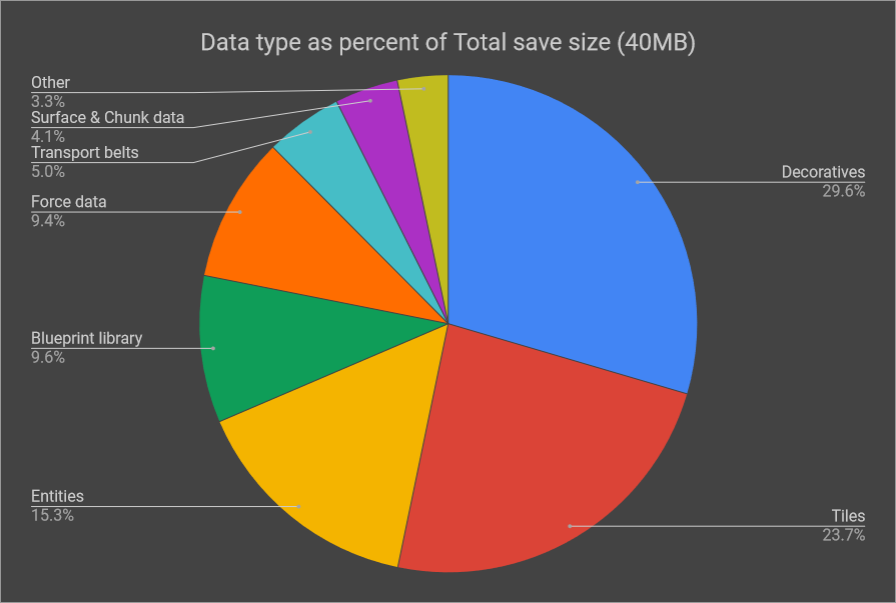
\includegraphics[width=0.9\textwidth]{images/factorio_save_statistic.png}
    \caption{Anteil der Datentypen beim Speichern\cite{factorioFridayFacts270}}
    \label{fig:factorioSaveStatistic}
\end{figure}



\subsection{Datenaufteilung} \label{ssec:factorioDatenaufteilung}
Die Spieldaten werden auch nach einem Chunk-basierten System getrennt. Dabei besteht ein Chunk aus einer Fläche von 32 mal 32 Tiles. Chunks werden für unterschiedliche Funktionen verwendet. Zum einen für die Generierung der Spielwelt. Jedes mal, wenn der Spieler neue Gebiete entdeckt, werden die Chunks dieser Gebiete generiert und angezeigt. Außerdem werden Chunks geladen und entladen, je nach Aktivitätsstatus dieser. Wenn bei einem Chunk nichts wichtiges mehr passiert, dann wird dieser im nächsten Tick\footnote{Ein Tick ist die kleinste Zeiteinheit in Factorio\cite{factorioTime}} ausgeschaltet, um Ressourcen zu sparen. Umweltverschmutzung, die Verbreitung von Umweltverschmutzung und die Ausbreitung der Gegner wird auch Chunk-basiert gehandhabt. 
\cite{factorioMapStructure}


\iffalse
\subsection{Ordnerstruktur}
User data Ordner:
\begin{itemize}
    \item ./saves (Save files)
    \item ./mods (Mods)
    \item ./script-output (Script-output, z.B. von Spiel Screenshots)
    \item ./scenarios (Lokale Szenarien)
    \item ./config/config.ini (Lokale Einstellung)
    \item factorio-*.log (Log files)
    \item factorio-dump-*.dmp (Crash dump files)
\end{itemize}

%2.8.2023
\url{https://wiki.factorio.com/Application_directory} 



\subsection{Speicherformate}
\url{https://wiki.factorio.com/index.php?title=Achievement_file_format&oldid=179094}\\
\url{https://wiki.factorio.com/index.php?title=Blueprint_string_format&oldid=190672}\\
\url{https://wiki.factorio.com/index.php?title=Map_exchange_string_format&oldid=187695}\\
\fi


\subsection{Speichervorgänge}
Factorio verwendet ein deterministisches Speicher- und Ladesystem. Das heißt, dass, egal welche Speicherdatei verwendet wird, der Speicher- und Ladeprozess für diesen Spielstand immer derselbe ist. Dieses System hat einige Vorteile für den Mehrspielermodus und das Wiedergabesystem von Factorio. Außerdem gibt es nicht jedes mal zufällige Veränderungen, beim erneuten Laden des letzten Spielstandes.\cite{factorioGithubSaveLoad}

Der Speicherprozess von Factorio besteht aus vielen kleinen Schritten. Zusammengefasst wird als erstes die ID-Mapping des Spielstandes und danach die Map-Daten gespeichert.
\cite{factorioFridayFacts270} Dabei werden die einzelnen Daten binär serialisiert.\cite{factorioGithubSaveLoad} Was passiert genau in diesen zwei Schritten? 

Der Speicherprozess beginnt als allererstes damit, dass die Garbage Collection von allen Lua-Zuständen geleert wird. Damit kann sichergestellt werden, dass keine Objekte gespeichert werden, die eigentlich nicht gesichert werden müssen.\cite{factorioGithubSaveLoad}

Als nächstes wird eine ScopedCallback-Klasse erstellt. Diese wird immer am Ende des Prozesses gelöscht und ruft dann eine "postSaveHook"-Funktion auf. Diese Funktion löscht temporäre Daten, die beim Speicherprozess entstanden sind. Der Vorteil dieser Funktion ist, dass diese immer aufgerufen wird, egal ob der Prozess erfolgreich oder mit einem Fehler terminiert hat. Damit kann sichergestellt werden, dass die Map-Daten nicht in einen beschädigten Zustand bleiben.\cite{factorioGithubSaveLoad}

Anschließend werden die ID-Mapping gespeichert.\cite{factorioGithubSaveLoad} Die ID-Mapping ist eine Liste, die jedem Spielobjekt eine Identifikationsnummer zuweist. Die ID-Mapping besteht dann aus der Identifikationsnummer und den zugehörigen Namen des Spielobjektes als Zeichenkette. Wie so eine ID-Mapping aussieht ist in der Abbildung \ref{fig:factorioIdMapping} zu sehen. Jeder Spielstand kann eine unterschiedliche ID-Mapping besitzen und diese kann sich oft verändern. Deshalb muss diese Liste jedes mal gespeichert werden.\cite{factorioFridayFacts259}

\begin{figure}[htp]
    \centering
    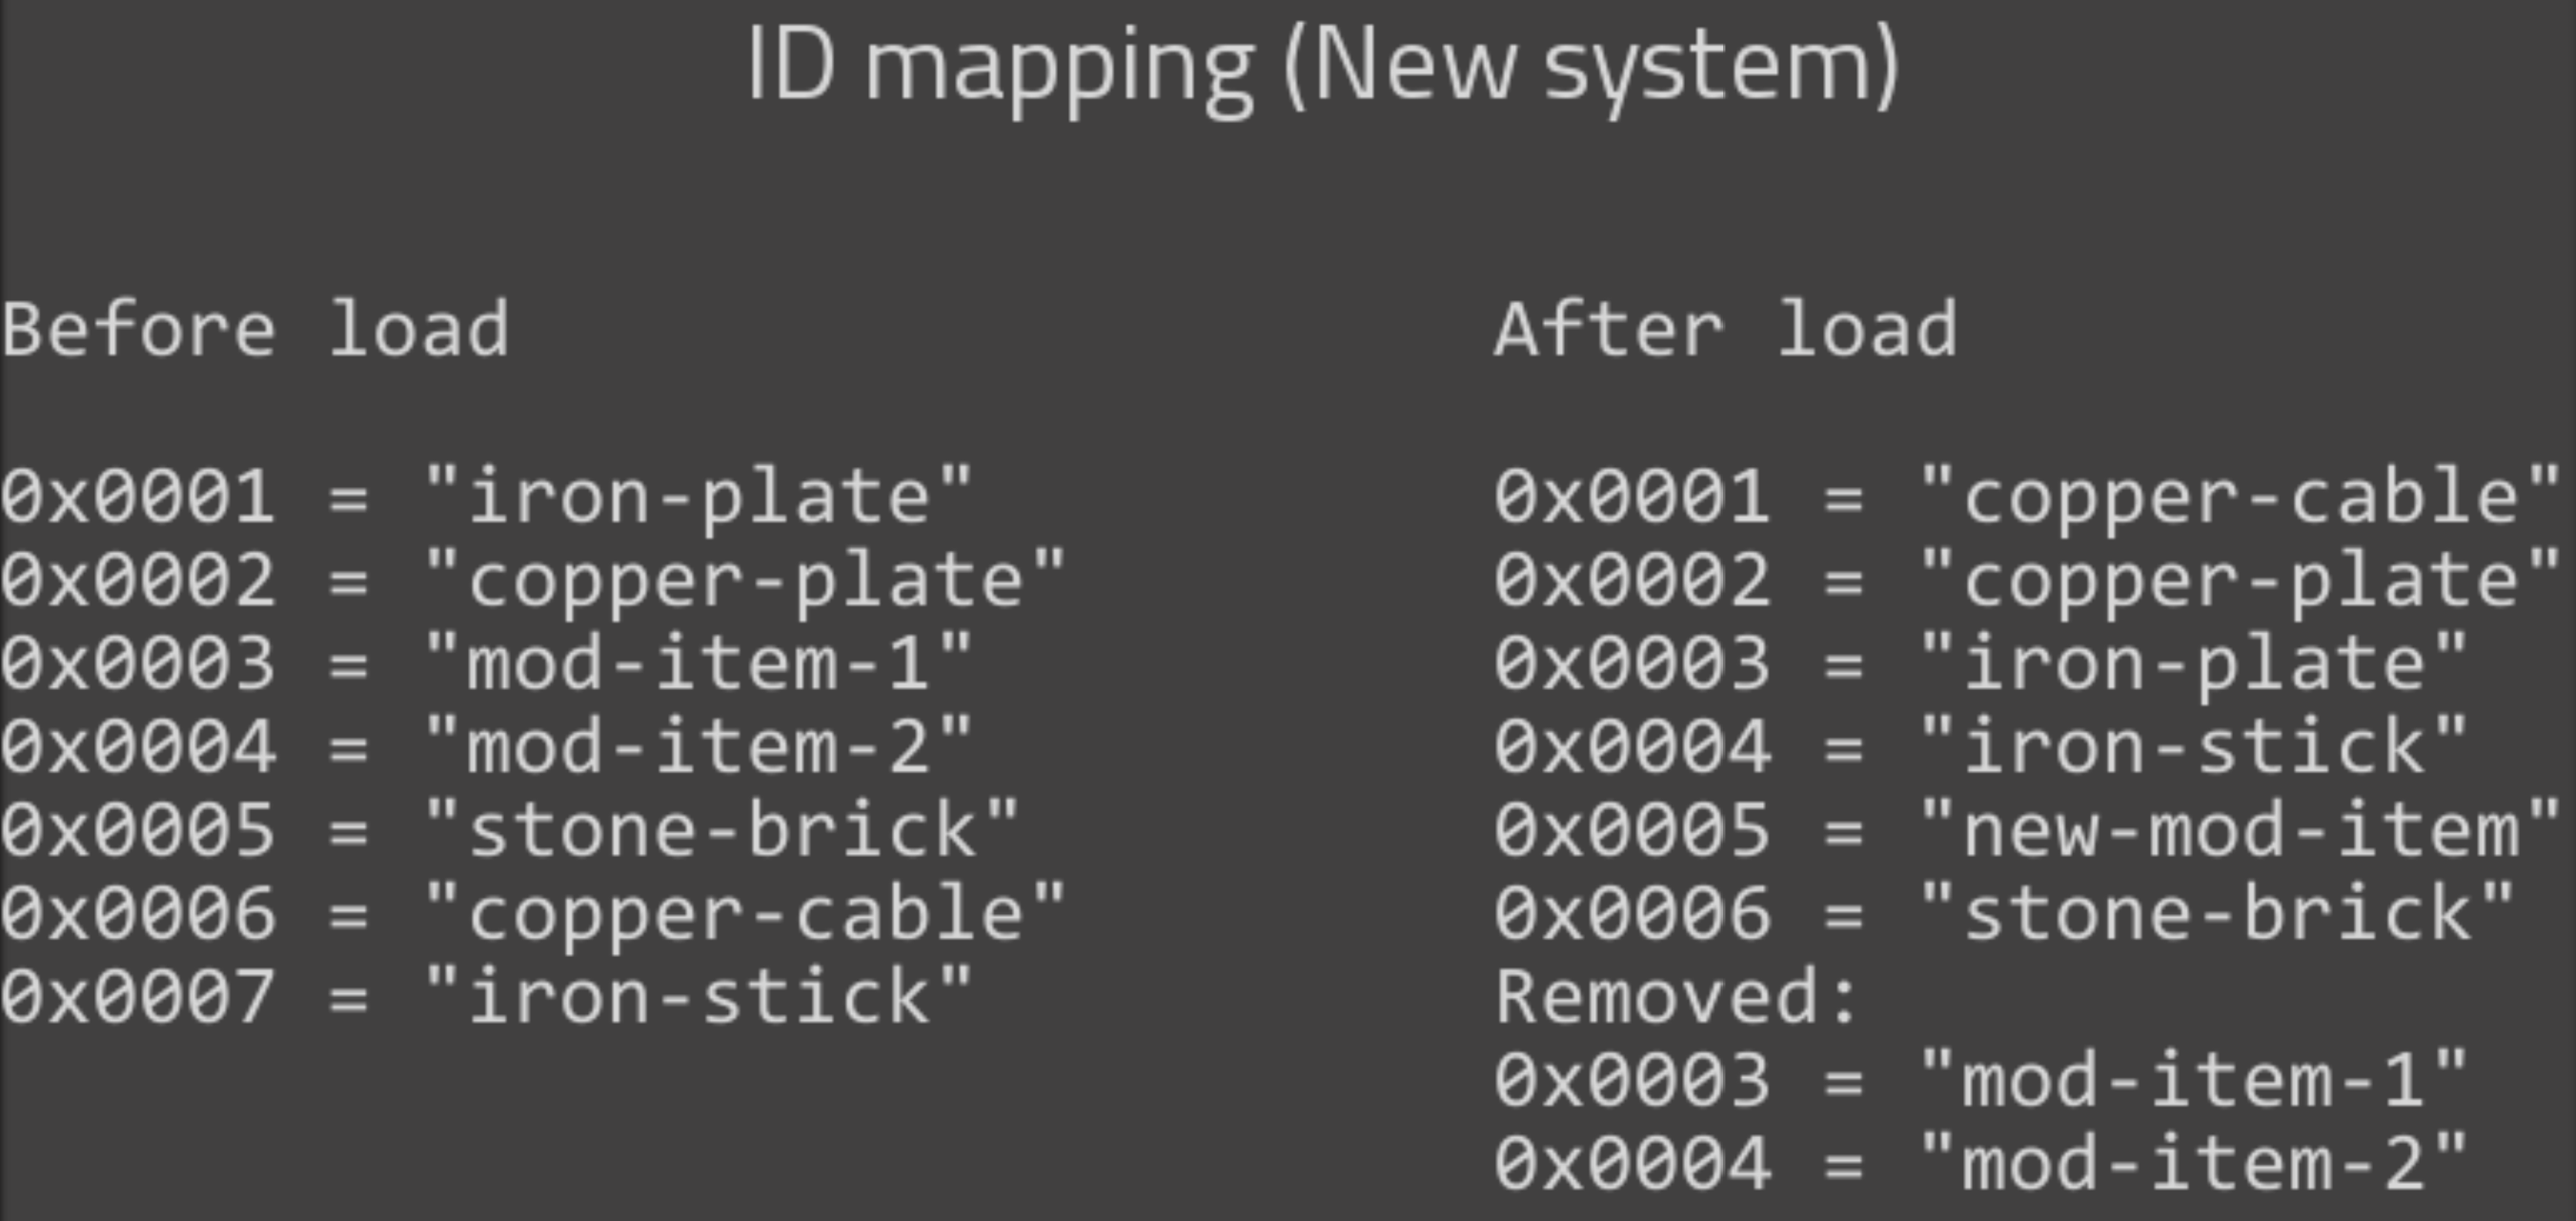
\includegraphics[width=0.9\textwidth]{images/id_mapping_factorio.png}
    \caption{Spielobjekte und deren Identifikationsnummer eines Spielstands\cite{factorioFridayFacts259}}
    \label{fig:factorioIdMapping}
\end{figure}

Als nächstes werden die angewandten Prototyp-Migrationen gesichert.\cite{factorioGithubSaveLoad} Ein Prototyp ist eine Vorlage für Maschinen, Rezepte und andere Spielkonzepte in der Factorio Game Engine.\cite{factorioPrototypesDocs}

Anschließend werden restliche Daten, die noch gespeichert werden müssen, gesichert und die SaveHelper-Liste wird abgearbeitet. Das SaveHelper-System wird verwendet, um weitere Speicherprozesse auszuführen, nachdem alles gespeichert wurde. Dafür muss ein SaveHelper erstellt werden, der dann durch das SaveHelper-System in eine Warteschlange von SaveHelpern hinzugefügt wird. Diese Warteschlange wird am Ende des Speicherprozesses abgearbeitet und von jedem SaveHelper wird die "save"-Funktion aufgerufen.\cite{factorioGithubSaveLoad}



\subsection{Ladevorgänge}
Der Ladeprozess für Factorio ist etwas komplizierter. Es gibt einige Dinge, die beachtet werden müssen, wie das Überprüfen der Map-Version und die Migration dieser auf andere Versionen. Außerdem muss überprüft werden, ob es bei den Mods Veränderungen gab. Factorio bietet Entwicklern an, Modifikationen des Spieles zu programmieren. Diese Modifikationen, auch "Mods" genannt, können zu einem Spielstand hinzugefügt werden. Deshalb muss bei jedem Laden des Spielstandes überprüft werden, ob Mods hinzugefügt, gelöscht oder verändert wurden. Worauf auch geachtet werden muss, ist, ob es beschädigte oder invalide Speicherdateien gibt.\cite{factorioFridayFacts270} 
Wie sieht dann der komplette Ladeprozess von Factorio aus, damit all diese Faktoren beachtet werden?

Der erste Schritt beim Laden eines Spielstandes ist, dass die Map-Version der zu ladenden Map mit der Version der Map, in die die Daten geladen werden sollen, verglichen werden muss. Falls die Versionen unterschiedlich sind, muss die zu ladende Map auf der Version der Map, in die geladen wird, migriert werden. Dabei muss beachtet werden, dass nicht jede Version von Factorio unterstützt wird. Manche Versionen können zu alt oder zu neu sein und können damit nicht verwendet werden.\cite{factorioGithubSaveLoad}

Als nächstes muss überprüft werden, ob die Mods, die für den zu ladenden Spielstand aktiv sind, oder die Mod-Einstellung sich geändert haben. Falls dies der Fall ist, müssen zusätzliche Vorgänge vorgenommen werden, nachdem die Daten geladen wurden. Dafür wird die Flag "prototype data changed" in der Lade-Klasse gesetzt.\cite{factorioGithubSaveLoad}

Bevor irgendwas geladen wird, was eine Identifikationsnummer benutzt, muss die ID-Mapping geladen werden. Ohne diesen Schritt weiß das Programm nicht, welches Spielobjekt mit welcher Identifikationsnummer gespeichert wurde und es könnte zu fehlerhaftes Laden des Spielstand führen. Außerdem wird über diesen Schritt dem Programm vermittelt, welche Spielobjekte sich verändert haben oder gelöscht wurden. Falls Mods die Identifikationsnummer von Spielobjekten zu anderen Identifikationsnummer ändern wollen, geschieht das auch direkt am Anfang.\cite{factorioGithubSaveLoad}

Nachdem die Identifikationsnummern erfolgreich geladen und gegebenenfalls modifiziert wurden, können die Standard-Map Daten geladen werden. Diese beinhalten Entitäten, Chunks, physikalische Kräfte und Züge.\cite{factorioGithubSaveLoad}

Wenn dieser Prozess abgeschlossen hat werden die LoadHelpers geladen. LoadHelpers arbeiten genau wie SaveHelpers, nur dass bei denen eine "load"-Funktion aufgerufen wird. Die SaveHelpers werden auch erst dann abgearbeitet, wenn die ganzen Daten geladen wurden. Die Reihenfolge der Prozesse der LoadHelpers muss genau gespiegelt zu der Reihenfolge der Prozesse der SaveHelpers ablaufen.\cite{factorioGithubSaveLoad}

Beim Ladeprozess gibt es Spielobjekte, die gelöscht werden müssen, aber dies kann erst passieren, wenn der Ladeprozess terminiert ist. Diese Spielobjekte können jetzt ohne Sicherheitsprobleme gelöscht werden. Außerdem werden jetzt noch Entitäten hinzugefügt, bei denen das Laden deren Daten fehlerhaft war. Dies muss jetzt geschehen, da beim Laden der Daten sich zum Beispiel Chunks verändern können, was zu Problemen bei manchen Entitäten führen kann. Wenn diese nochmal geladen werden, werden diese Probleme überschrieben und gelöst.\cite{factorioGithubSaveLoad}

Eine weitere Funktion, die die LoadHelpers besitzen, ist die "setup"-Funktion. Als nächsten Schritt wird von allen LoadHelpers diese Funktion aufgerufen. In der Setup-Funktion ist Logik, die nach der Load-Funktion und vor der Setup-Funktion der einzelnen Entitäten ausgeführt werden soll.\cite{factorioGithubSaveLoad}

Falls die "prototype data changed"-Flag gesetzt wurde, müssen die Daten zum Stromnetz noch einmal gelöscht und neu berechnet werden. Wenn die Flag gesetzt wurde, kann es sein, dass die Begrenzung von Entitäten sich verändert hat. Damit kann sich auch das Stromnetz, in dem sich eine Entität befindet, verändert haben, weshalb diese Daten in diesem Fall noch einmal neu berechnet werden.\cite{factorioGithubSaveLoad}

Als nächstes wird die Setup-Funktion aller Entitäten aufgerufen. Dabei werden als Erstes die Setup-Funktionen aller Transportbänder und danach die der restlichen Entitäten aufgerufen. Diese Reihenfolge ist wichtig, da die Logik des Zusammenführens der Entitäten mit den Transportbändern, die Entitäten durchführen, die keine Transportbänder sind. Dafür sollten alle Transportbänder schon fertig eingerichtet sein. Falls neue Entitäten beim Aufrufen der Setup-Funktionen entstehen, müssen auch bei diesen deren Setup-Funktion aufgerufen werden.\cite{factorioGithubSaveLoad}

Anschließend wird die Funktion "postLoadHook" aufgerufen. Diese geht nochmal über jede Oberfläche der Spielwelt und stellt die Liste der aktiven Entitäten wieder her. Da beim vorherigen Schritt neue Entitäten entstehen können, kann die "postLoadHook"-Funktion erst jetzt aufgerufen werden.\cite{factorioGithubSaveLoad} 

Als nächstes werden alle Tiles überprüft, da manche Veränderungen der Tiles beim Ladeprozess andere Tiles invalide machen können. Diese Tiles müssen gelöscht werden und auch alle Entitäten, die auf diesen liegen. Das Löschen von Entitäten ist jedoch erst dann möglich, wenn diese fertig eingerichtet wurden, also nach dem Aufruf der Setup-Funktion. Anschließend werden die Oberflächen- und Zug-Daten eingerichtet.\cite{factorioGithubSaveLoad}

Jetzt können die Veränderungen durchgeführt werden, die abgearbeitet werden müssen, wenn die "prototype data changed"-Flag gesetzt wurde. Dafür gibt es Entitäten, die mit "alarmed" markiert wurden. Diesen muss jetzt weitergegeben werden, dass alle die Entitäten fertig eingerichtet wurden und die Veränderungen beginnen können.\cite{factorioGithubSaveLoad}

Zum Schluss werden alle Dummy-Objekte gelöscht, letzte Setup-Funktionen aufgerufen und die Lua-Daten geladen und wiederherstellt. Dummy-Objekte werden in einer Liste während des Ladeprozesses gesammelt. Ein Objekt wird zu dieser Liste hinzugefügt, wenn dieses Objekt während des Ladevorgangs migriert oder gelöscht wurde. Die Liste der Dummy-Objekte wird dann am Ende abgearbeitet, damit die Objekte endgültig ohne Sicherheitsprobleme entfernt werden können.\cite{factorioGithubSaveLoad}

Wie zu sehen ist, ist der Ladeprozess von Factorio um einiges aufwendiger als der Speicherprozess. Der Ladeprozess besteht noch aus ein paar weiteren Schritten, diese sind aber für das Verständnis des gesamten Ladeprozesses nicht relevant. Was auch zu erkennen ist, ist, dass der Ladeprozess aus wiederholtem laden, einrichten, beheben von Problemen und neu berechnen besteht. Da stellt sich die Frage, ob dies effizient gelöst wurde, oder ob die teilweise wiederholten Schritte gekürzt werden können. Vermutlich gibt es zu viele Abhängigkeiten bei der Reihenfolge der einzelnen Prozesse, weshalb wenig Spielraum für Optimierung vorhanden ist.\todo{Ladezeiten lang in der Realität?}



\subsection{Fazit}
\dots
%--------------------------------------------------------------------------



%--------------------------------------------------------------------------
\section{Stardew Valley}
Beschreibung von dem Spiel

\begin{itemize}
    \item Bauernhof aufbauen und darum kümmern 
\end{itemize}
\url{https://www.stardewvalley.net/press/}\\
\url{https://store.steampowered.com/app/413150/Stardew_Valley/}\\
\url{https://www.stardewvalley.net/faq/}

\todo{Manche Daten aus Save-Datei}

\subsection{Daten}
\begin{itemize}
    \item Player
    \begin{itemize}
        \item Name (Spielername, Farmname, Hundname, ...)
        \item Position
        \item Quest-Log (Quests die der Spieler offen hat)
        \item Items
        \item Aussehen (Klamotten, Haare, Hautfarbe, ...)
        \item etc.
    \end{itemize}
    \item Location (mehrere)
    \begin{itemize}
        \item Charaktere (mit Typ, Name, Position, ...)
        \item Objekte (mit Position, Name, Kategorie, Preis, ...)
        \item Terrain-Features (mit Schlüssel (Position) und Wert (Spielobjekt))
        \item Gebäude (mit Innenausstattung und Charaktere)
        \item etc.
    \end{itemize}
    \item Mailbox (nur ID der einzelnen Mails)
    \item Statistiken (wie viel Items gebaut wurden, wei viele Saatgut gesät wurde, ...)
    \item etc.
\end{itemize}

\subsection{Ordnerstruktur}
Die Ordnerstruktur von Stardew Valley ist recht schlicht gehalten, da die Anzahl der Daten im Vergleich zu den vorherigen Spielen klein sind. Für jede Spielwelt, die ein Spieler erstellt, gibt es einen eigenen Ordner. Der Name von diesem Ordner setzt sich aus dem Namen des Bauernhofs zusammen und eine Identifikationsnummer. In diesem Ordner sind dann vier Dateien. Die Dateien ohne der "\_old"-Endung haben den letzten Spielstand gespeichert und die mit dieser Endung den Spielstand davor. Dabei beinhalten die SaveGameInfo-Dateien Informationen, die im "Load Game"-Menü gebraucht werden. Die Daten zu einem Spielstand sind in der "<Bauernhof Name>\_<ID>"-Datei gespeichert, wobei der Name dieser Datei identisch zu dem des Ordners ist. Den kompletten Aufbau der Ordnerstruktur ist in der Abbildung \ref{lst:ordnerStrukturStardewValley} zu sehen. Die Daten in den Dateien werden im \ac{xml}-Format gespeichert, mehr dazu im Abschnitt \ref{ssec:speicherformateStardew}.\cite{stardewvalleywikiSaves}\cite{stardewvalleyFiles}

\begin{listing}[htp]
    \dirtree{%
    .1 <Bauernhof Name>\_<ID>.
        .2 \textcolor{blue}{SaveGameInfo}.
        .2 \textcolor{blue}{<Bauernhof Name>\_<ID>}.
        .2 \textcolor{blue}{SaveGameInfo\_old}.
        .2 \textcolor{blue}{<Bauernhof Name>\_<ID>\_old}.
    } 
    \caption{Ordnerstruktur einer Spielwelt in Stardew Valley}
    \label{lst:ordnerStrukturStardewValley}
\end{listing}

\subsection{Speicherformate} \label{ssec:speicherformateStardew}

\begin{itemize}
    \item XML-Format, siehe Listings
\end{itemize}

\begin{listing}[htp]
    \begin{minted}[breaklines,frame=single]{xml} 
        <?xml version="1.0" encoding="utf-8"?>
        <SaveGame
          xmlns:xsi="http://www.w3.org/2001/XMLSchema-instance"
          xmlns:xsd="http://www.w3.org/2001/XMLSchema">
          <player>
            <name>Spielername</name>
            ...
            <Position>
              <X>123</X>
              <Y>456</Y>
            </Position>
            ...
            <questLog>
              <Quest>...</Quest>
              <Quest>...</Quest>
              ...
            <questLog>
            ...
            <items>
                <Item xsi:type="Axe">...</Item>
                <Item xsi:type="Pickaxe">...</Item>
                ...
            </items>
            ...
            <farmName>Bauernhofname</farmName>
            ...
            <shirt>1</shirt>
            <hair>2</hair>
            <skin>3</skin>
          <player>
          <locations>
            <GameLocation xsi:type="FarmHouse">...</GameLocation>
            <GameLocation xsi:type="Farm">...</GameLocation>
            ...
          </locations>
          ...
        </SaveGame>
    \end{minted}
    \caption{Hauptdatei zum Speichern des Spielstandes}
    \label{lst:stardewvalleySaveGame}
\end{listing}

\begin{listing}[htp]
    \begin{minted}{xml} 
        <?xml version="1.0" encoding="utf-8"?>
        <Farmer
          xmlns:xsi="http://www.w3.org/2001/XMLSchema-instance"
          xmlns:xsd="http://www.w3.org/2001/XMLSchema">
          <name>Spielername</name>
          ...
          <Position>
            <X>123</X>
            <Y>456</Y>
          </Position>
          ...
          <questLog>
            <Quest>...</Quest>
            <Quest>...</Quest>
            ...
          <questLog>
          ...
            <farmName>Bauernhofname</farmName>
          ...
          <shirt>1</shirt>
          <hair>2</hair>
          <skin>3</skin>
          ...
        </Farmer>
    \end{minted}
    \caption{SaveGameInfo Datei}
    \label{lst:stardewvalleySaveGameInfo}
\end{listing}

\subsection{Datenaufteilung}
Alles in einer Datei, viele Spielobjekte nach GameLocation aufgeteilt (Quelle Listing)

\subsection{Speichervorgänge}
Die Speichervorgänge von Stardew Valley sind sehr schlicht gehalten. In der Spielwelt gibt es einen Tag-Nacht-Zyklus. Sobald der Spieler in dem Spiel in einem Bett, oder der Spielcharakter automatisch um zwei Uhr nachts schlafen geht, wird der komplette Spielstand abgespeichert. Falls das Programm vorher terminiert, ist der Spielstand des aktuellen Tages im Spiel verloren gegangen.\cite{stardewvalleywikiSaves}
%--------------------------------------------------------------------------



\iffalse
%--------------------------------------------------------------------------
\section{Terraria}

In \url{https://store.steampowered.com/news/app/105600/view/4560463273436543493} steht die neue offizielle Doku Seite für Terraria (\url{https://terraria.wiki.gg/wiki/Terraria_Wiki})


\subsection{Daten}
Welche Klassen gibt es bei Terraria (Blöcke, Chunks,...) und welche Daten 
beinhalten diese.

\subsection{Ordnerstruktur}

\subsection{Speicherformate}
World-Dateien, Player-Dateien, Konfigurationsdateien 

\subsection{Datenaufteilung}
Kein Chunksystem, alles in einer Datei gespeichert. Aber Inventar, Position
usw. werden in verschiedenen Daten gespeichert.

\subsection{Speichervorgänge}

\subsection{Ladevorgänge} 
%--------------------------------------------------------------------------



%--------------------------------------------------------------------------
\section{Ein Spiel}
Beschreibung von dem Spiel

\subsection{Daten}
Welche Klassen gibt es bei <Spielname> (Blöcke, Chunks,...) und welche Daten 
beinhalten diese.

\subsection{Ordnerstruktur}

\subsection{Speicherformate}

\subsection{Datenaufteilung}

\subsection{Speichervorgänge}

\subsection{Ladevorgänge}
\fi


    % Die nächsten zwei Zeilen sind optional, sie sorgen dafür dass alles nach dem Inhalt wieder mit römischen Zahlen nummeriert wird.
    \pagenumbering{roman}
    \addtocounter{page}{4} % Dies ist die Anzahl der Seiten vor der Einleitung, muss möglicherweise angepasst werden, wenn das Inhaltsverzeichnis mehrere Seiten umfasst.

    \bibliographystyle{alphadin}
    \bibliography{main}

    \listoffigures
    \listoftables
    \renewcommand{\listoflistingscaption}{Listing-Verzeichnis}
    \listoflistings

    \appendix
    \chapter{Anhang}\label{ch:appendix}

\begin{figure}[htp]
    \centering
    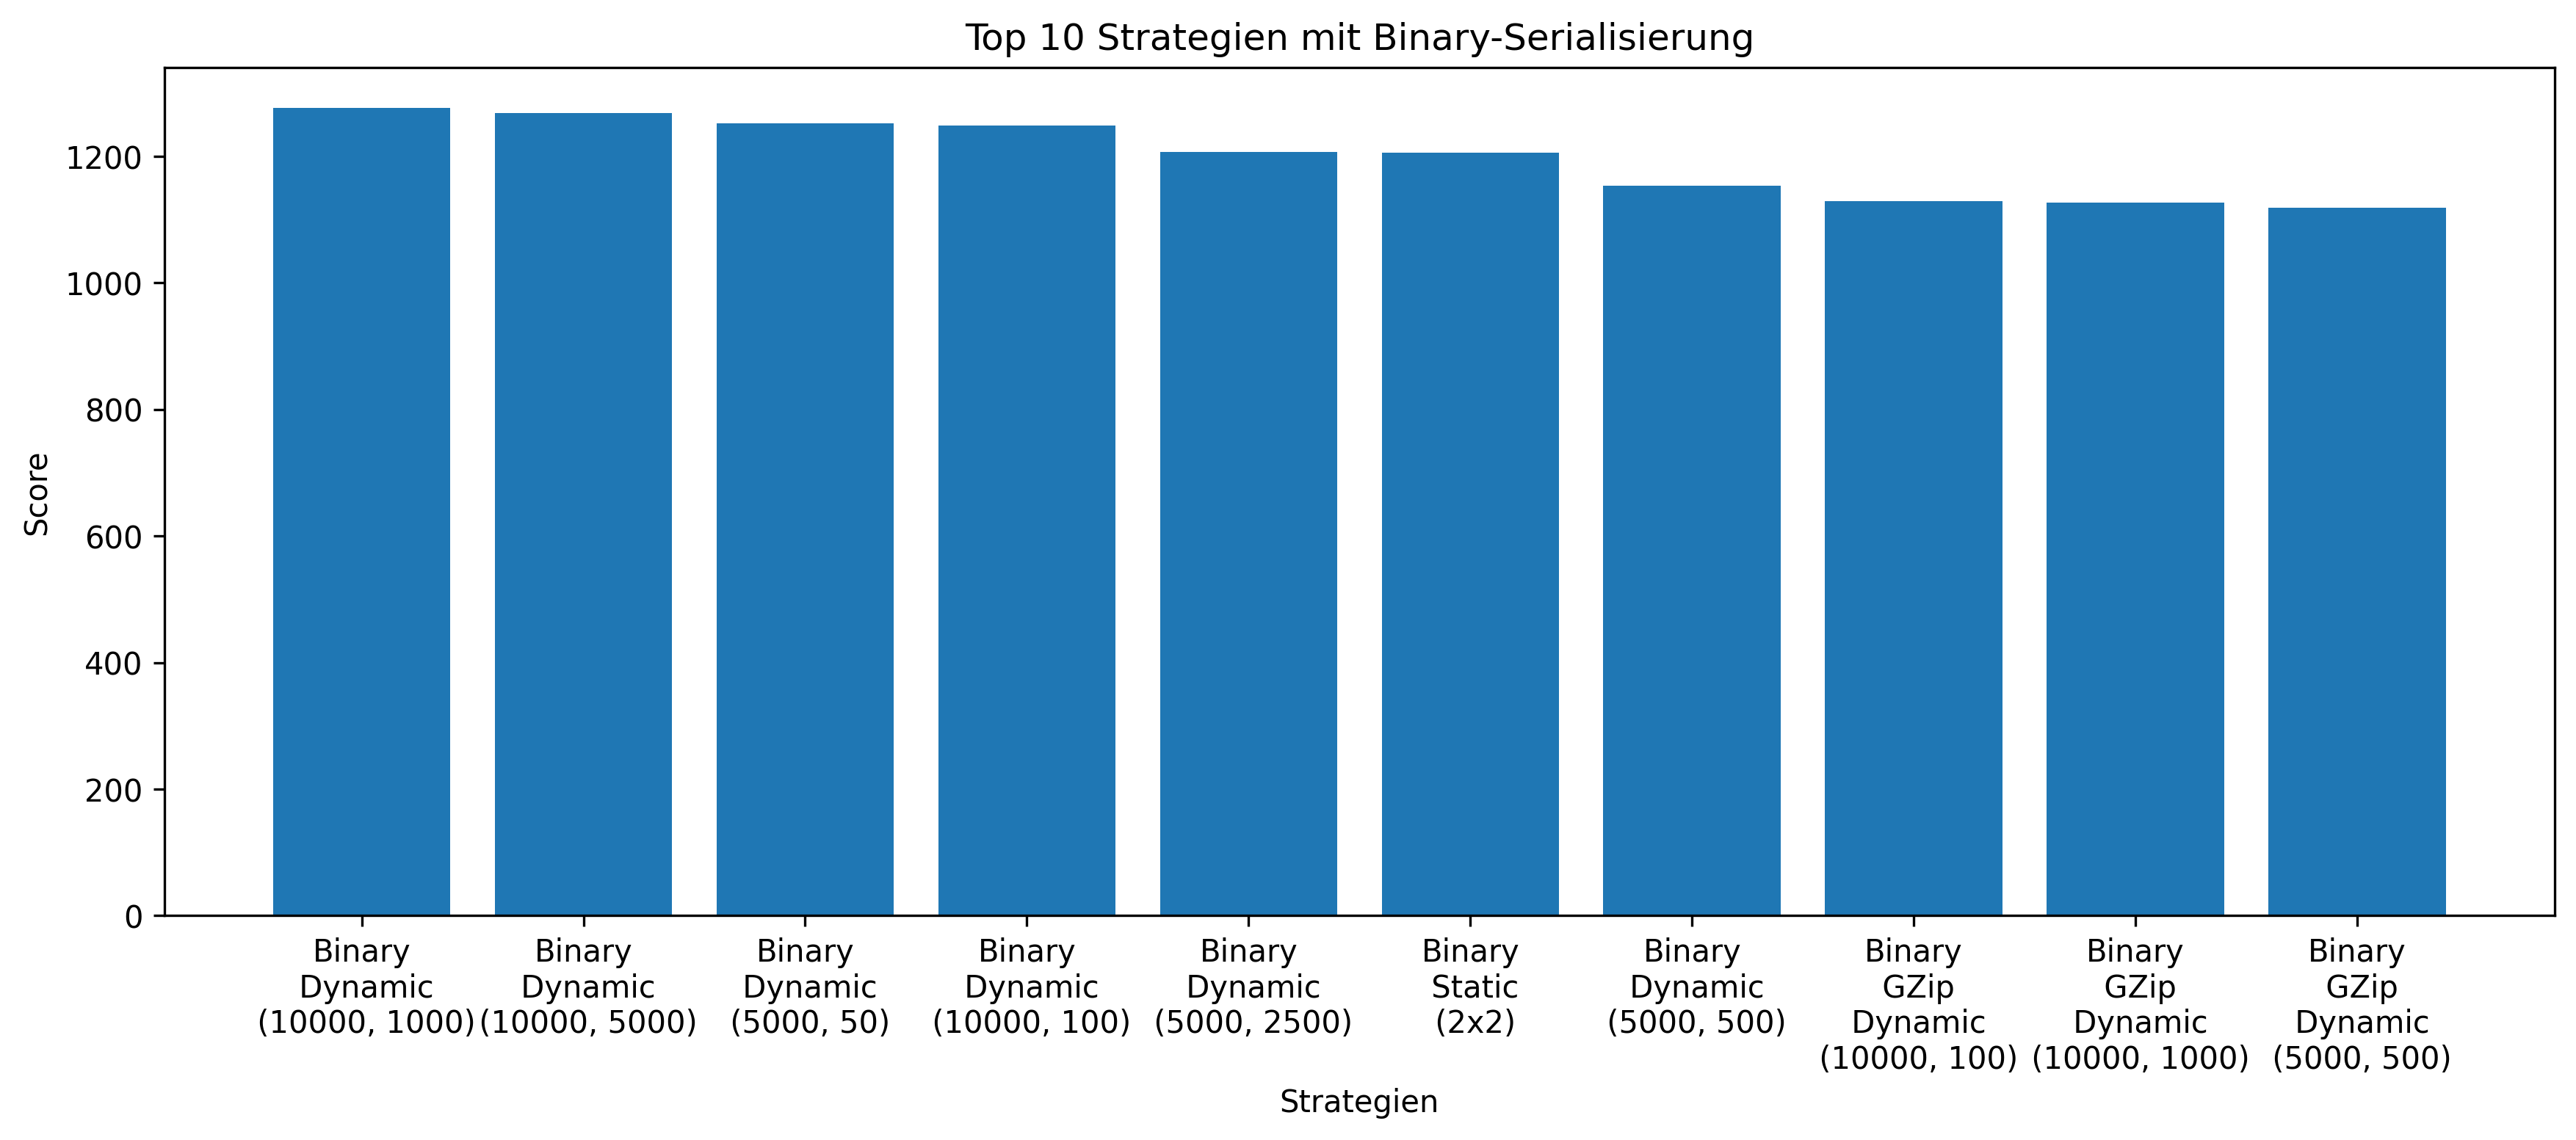
\includegraphics[width=1\textwidth]{images/plots/Binary.png}
    \caption{Beste Binären-Strategien nach dem Score-System aller Kategorien}
    \label{fig:topStratBin}
\end{figure}

\begin{figure}[htp]
    \centering
    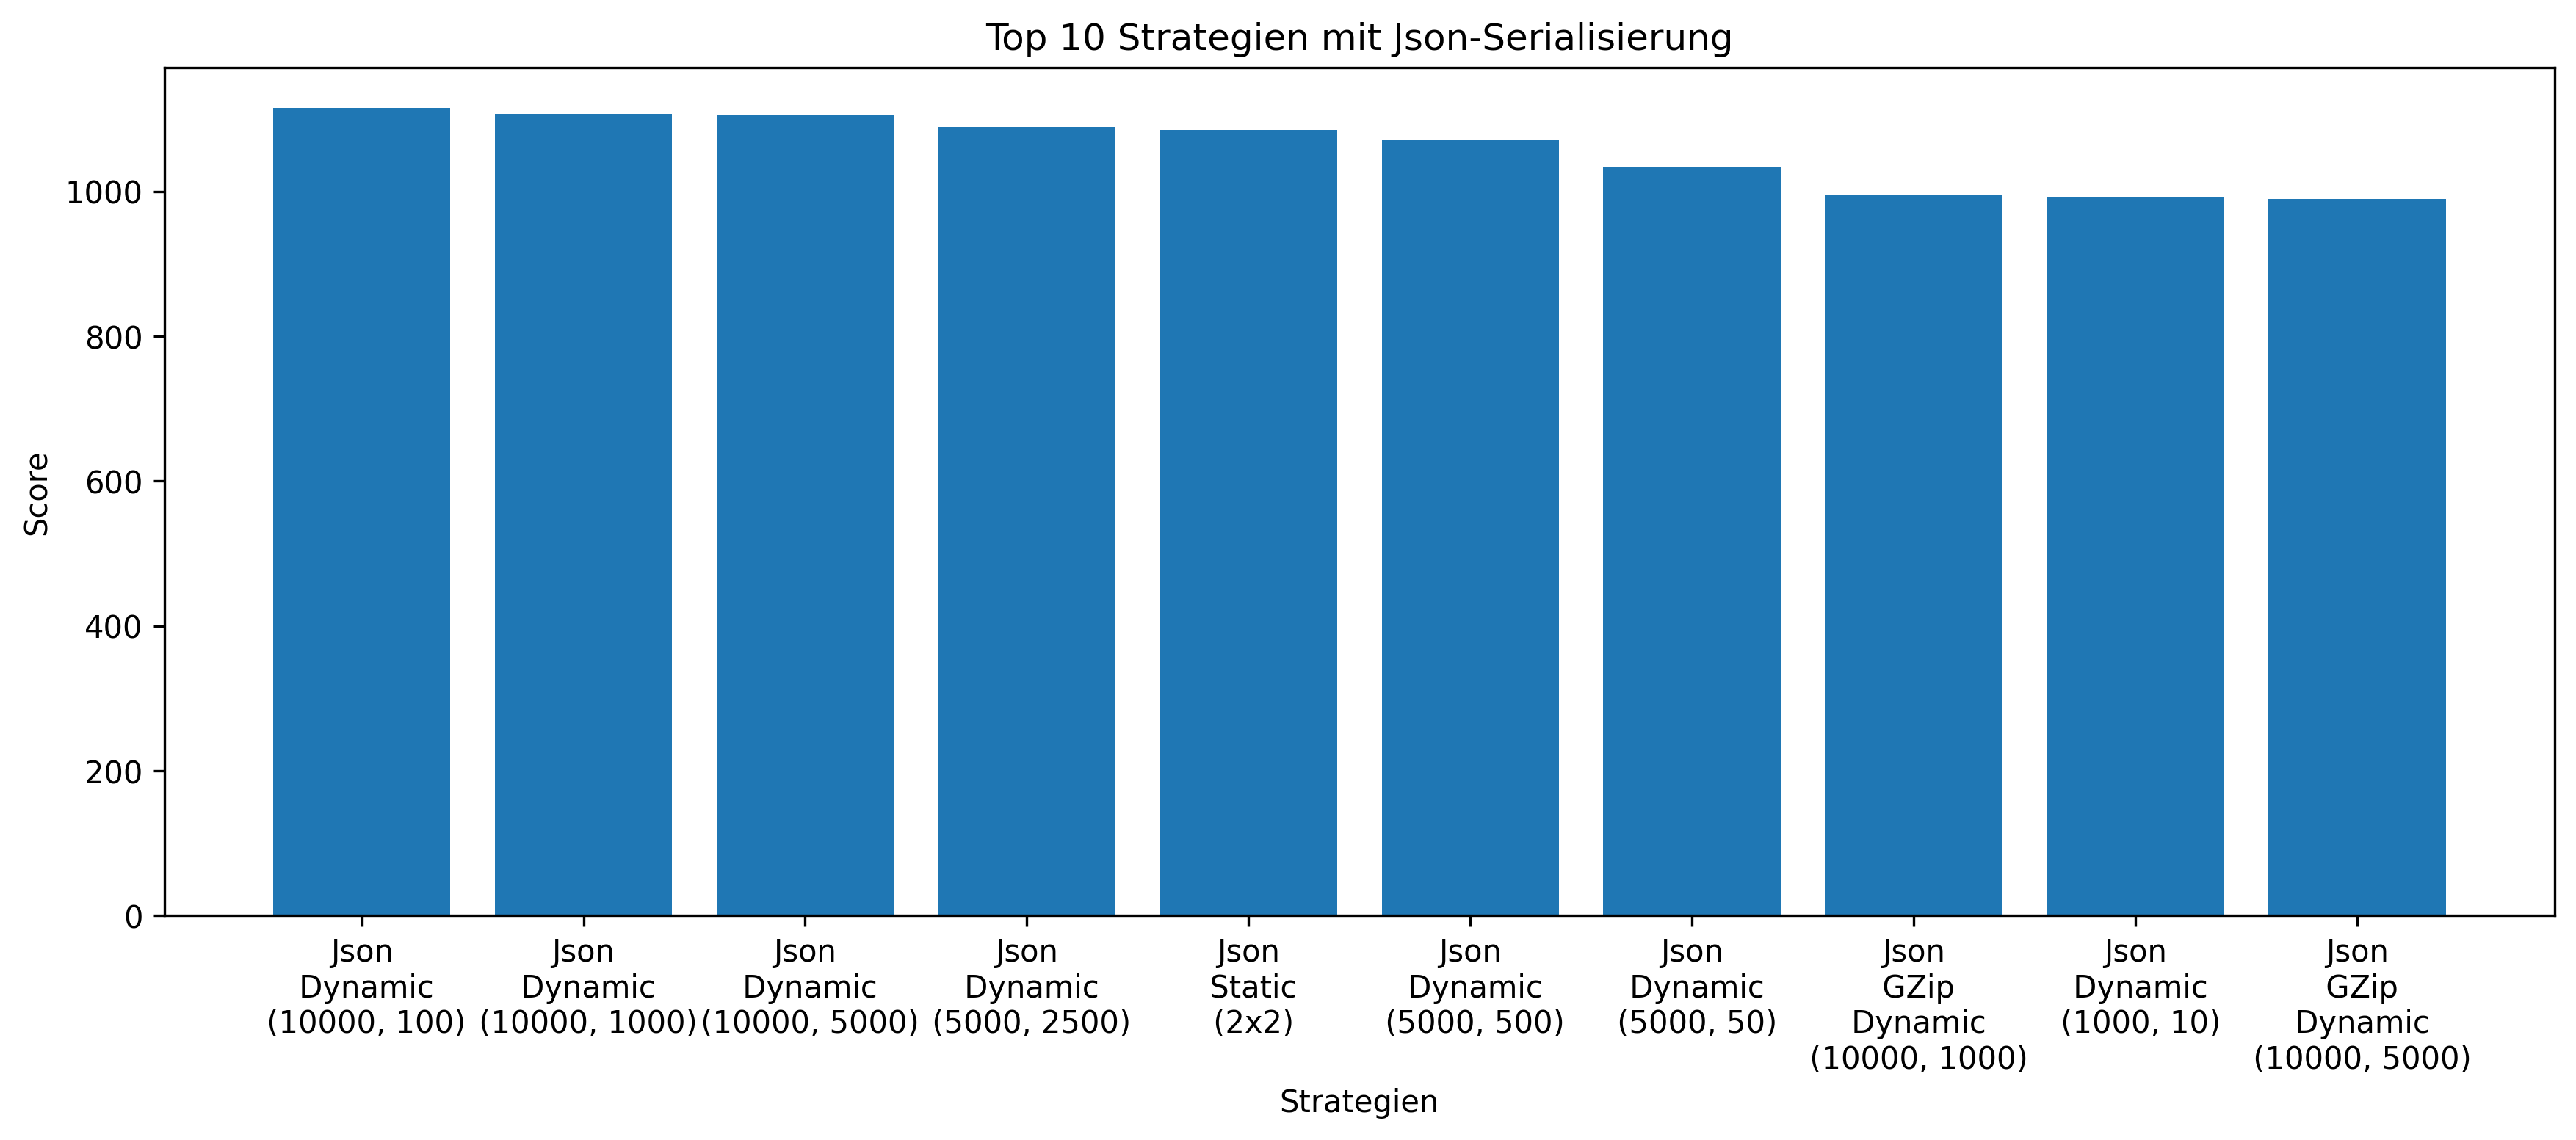
\includegraphics[width=1\textwidth]{images/plots/Json.png}
    \caption{Beste JSON-Strategien nach dem Score-System aller Kategorien}
    \label{fig:topStratJson}
\end{figure}

\begin{figure}[htp]
    \centering
    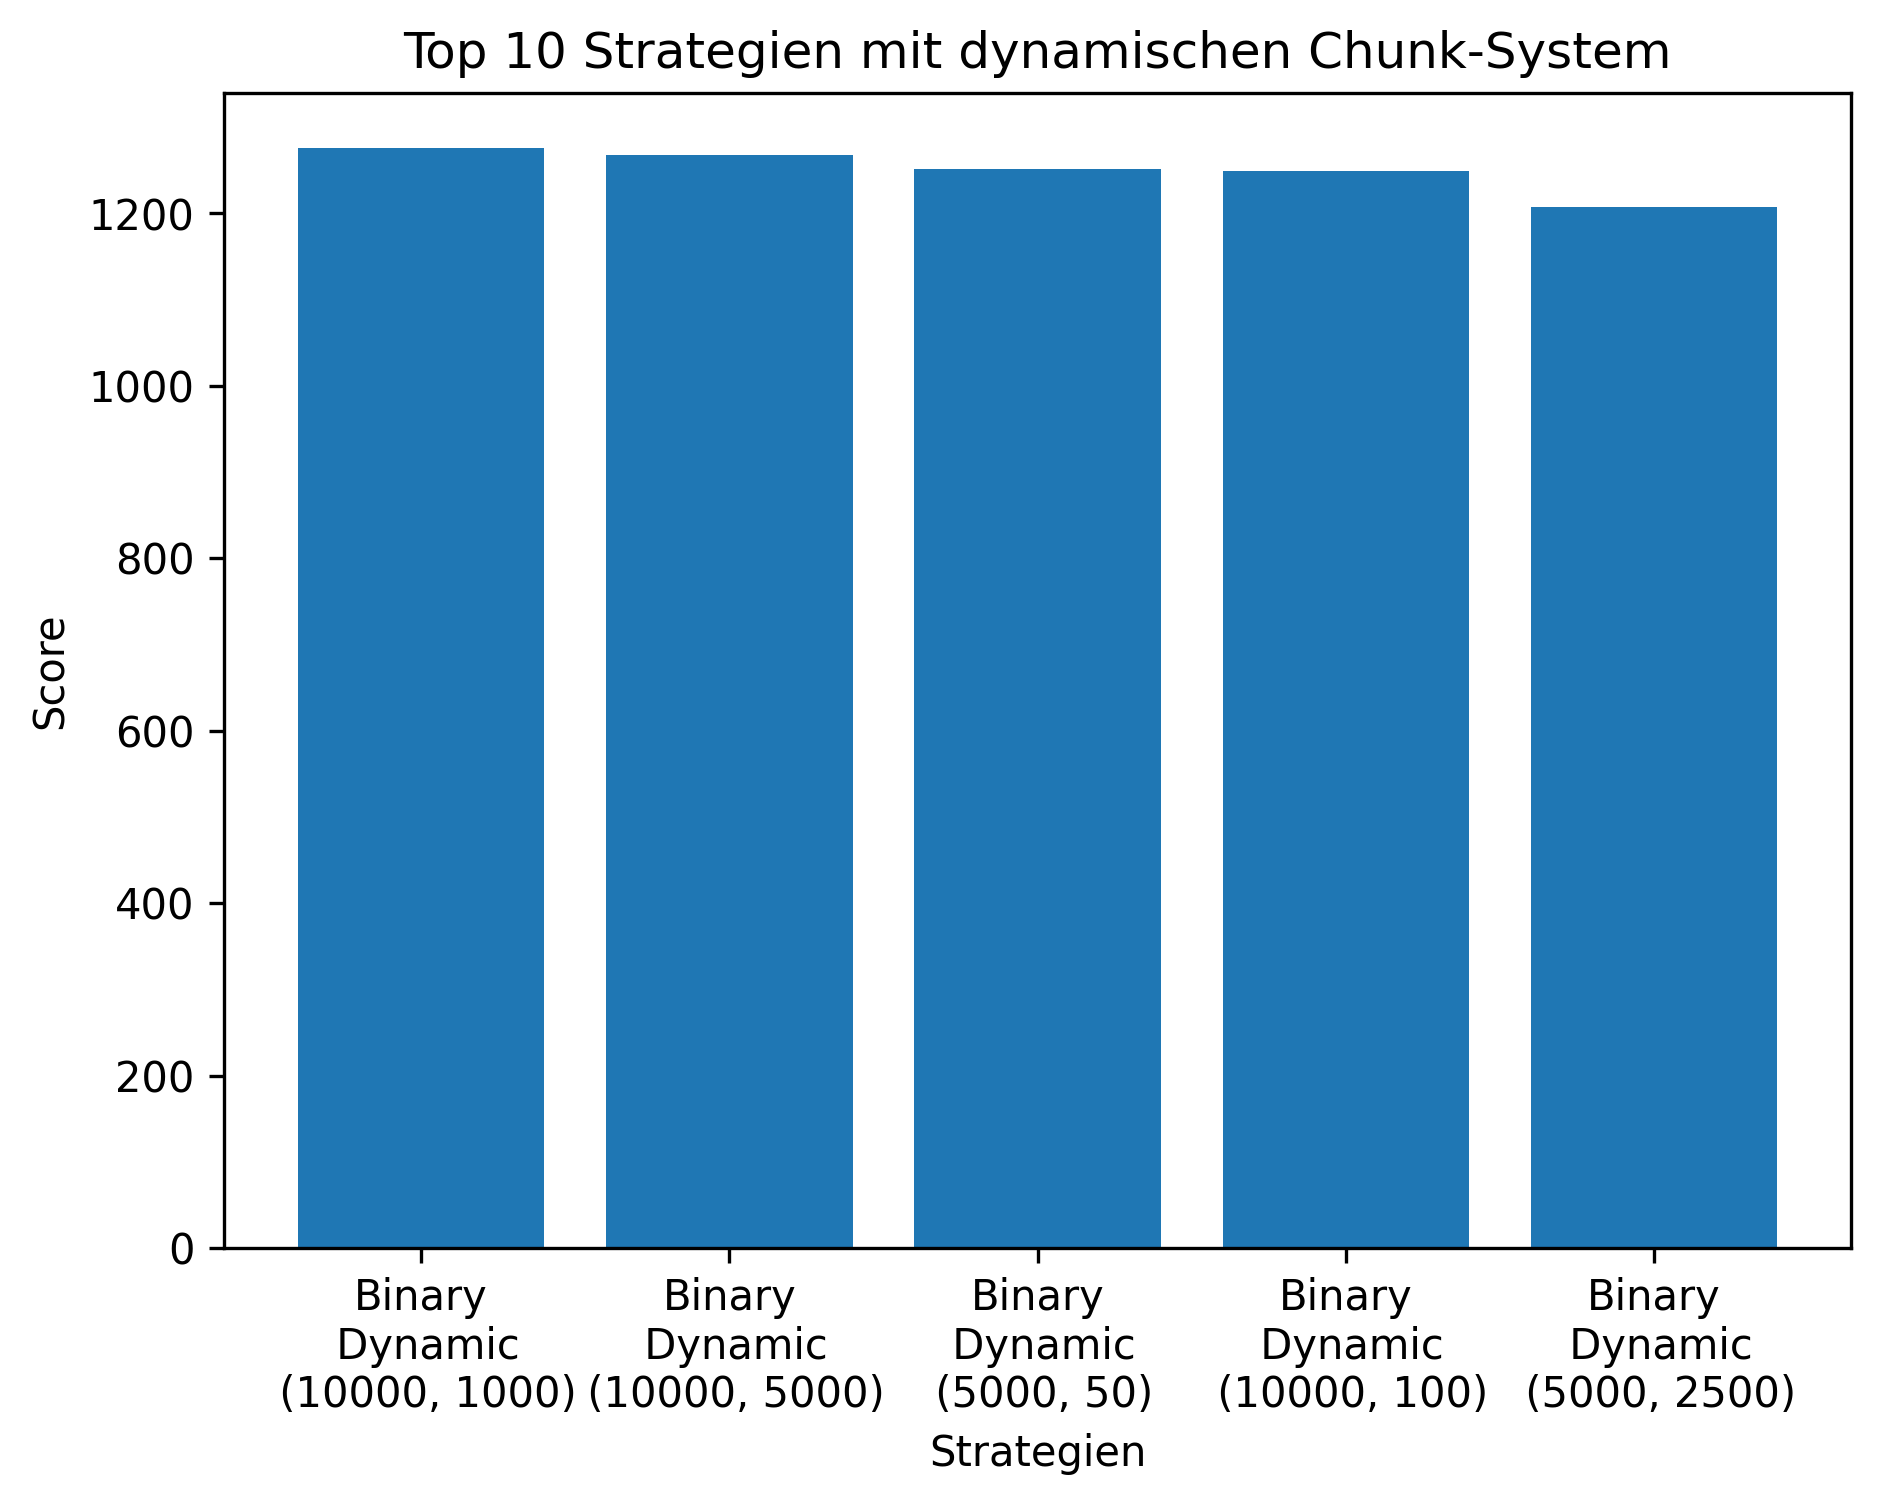
\includegraphics[width=0.7\textwidth]{images/plots/dynamisch.png}
    \caption{Beste Strategien mit dynamischen Chunk-System nach dem Score-System aller Kategorien}
    \label{fig:topDynamic}
\end{figure}

\begin{figure}[htp]
    \centering
    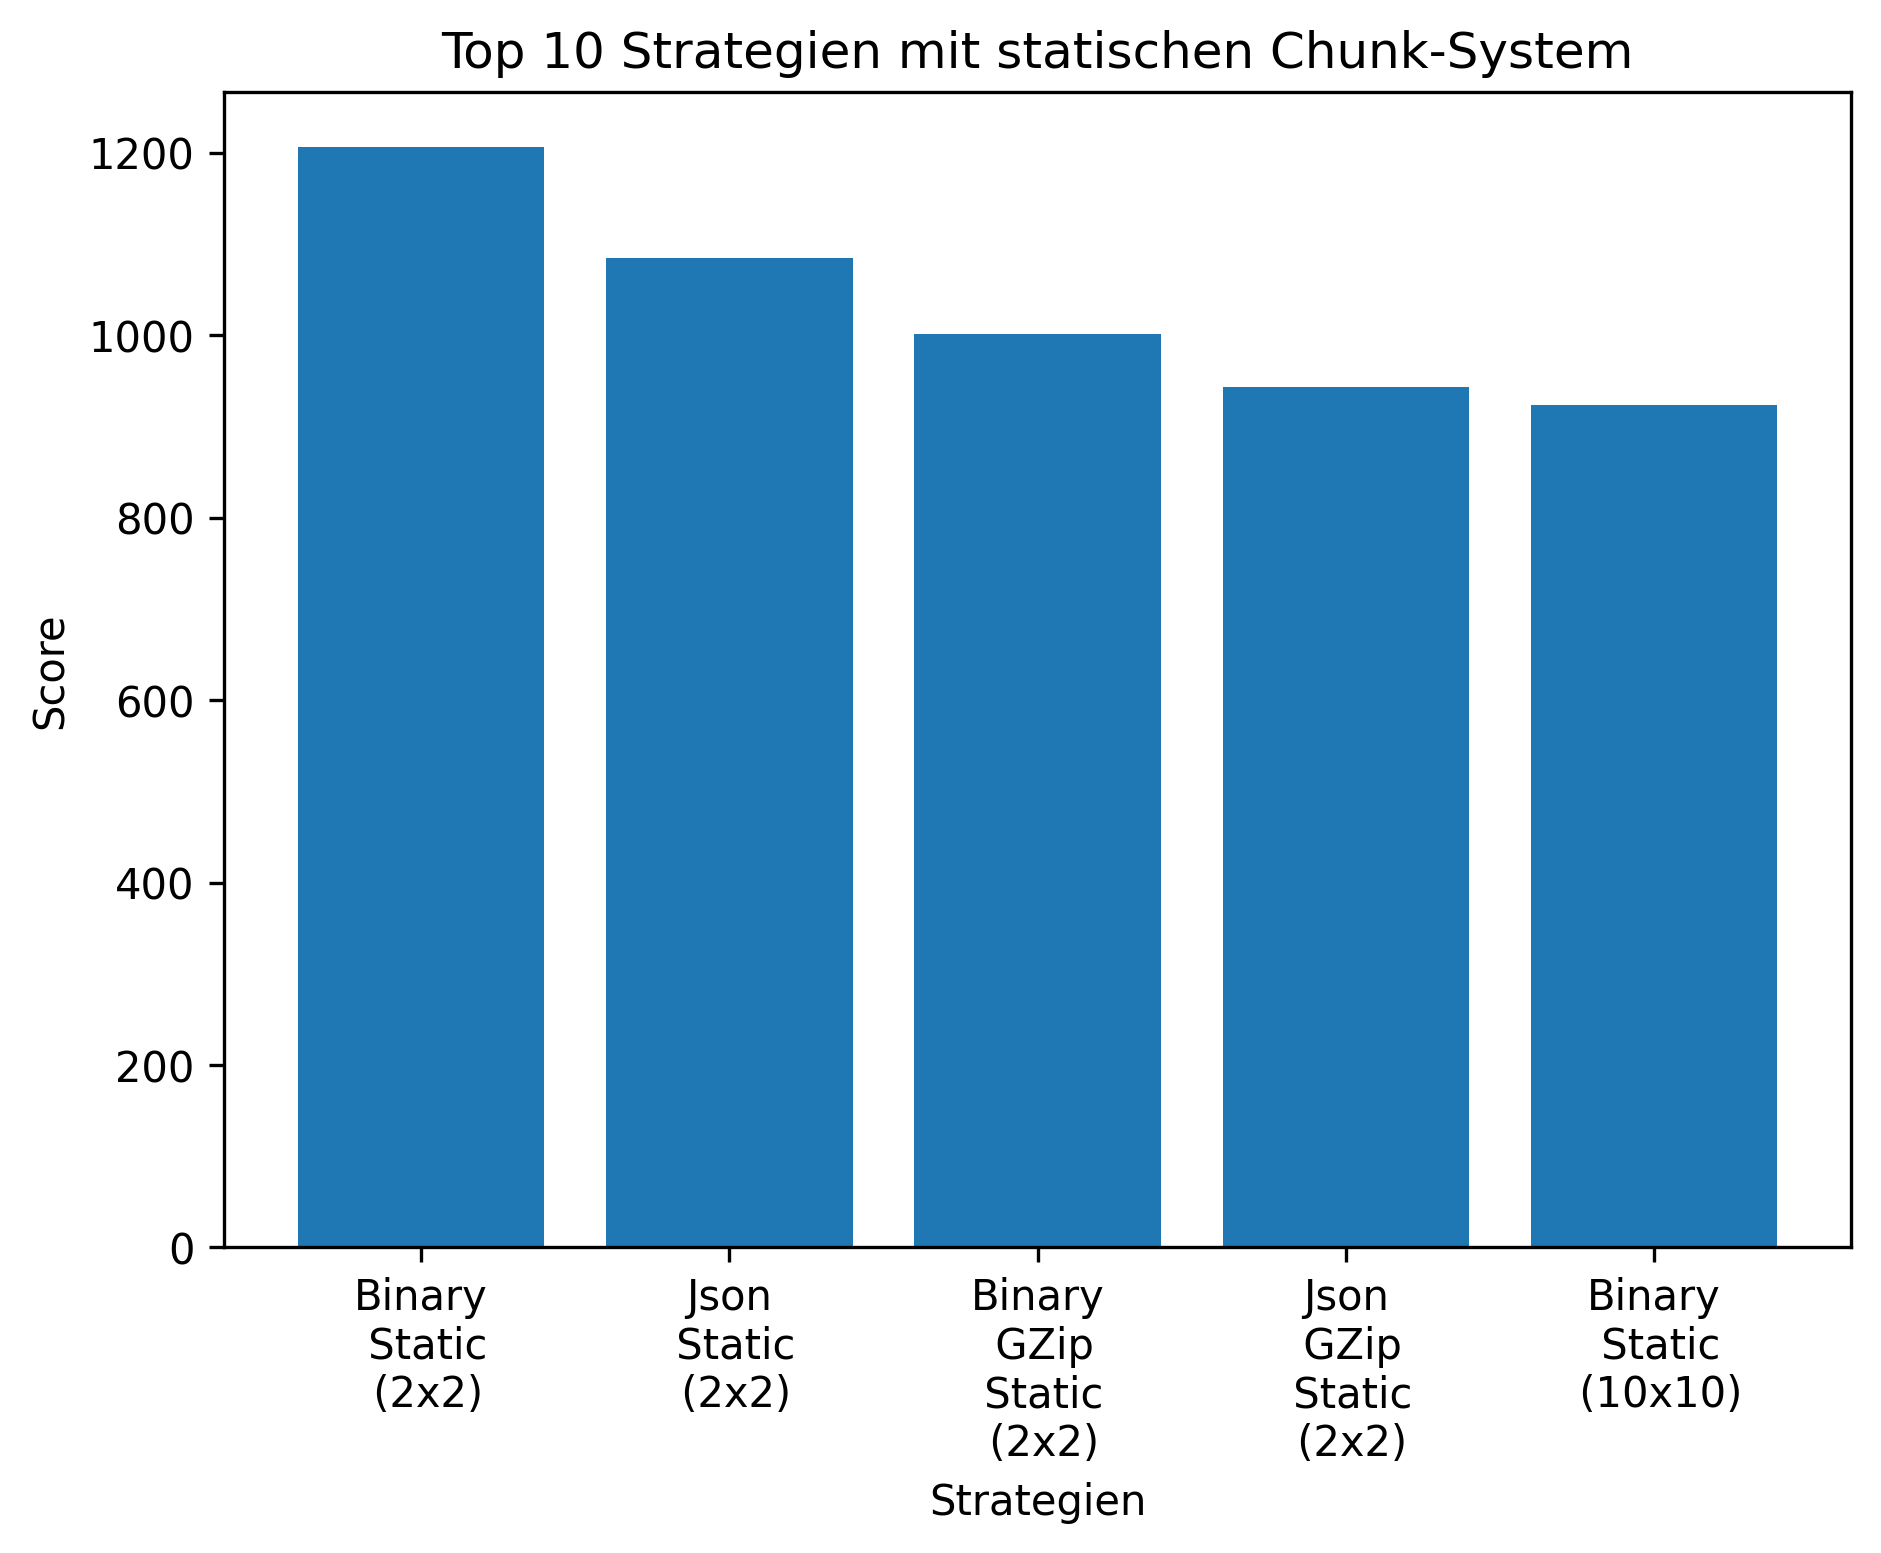
\includegraphics[width=0.7\textwidth]{images/plots/statisch.png}
    \caption{Beste Strategien mit statischen Chunk-System nach dem Score-System aller Kategorien}
    \label{fig:topStatic}
\end{figure}

\begin{figure}[htp]
    \centering
    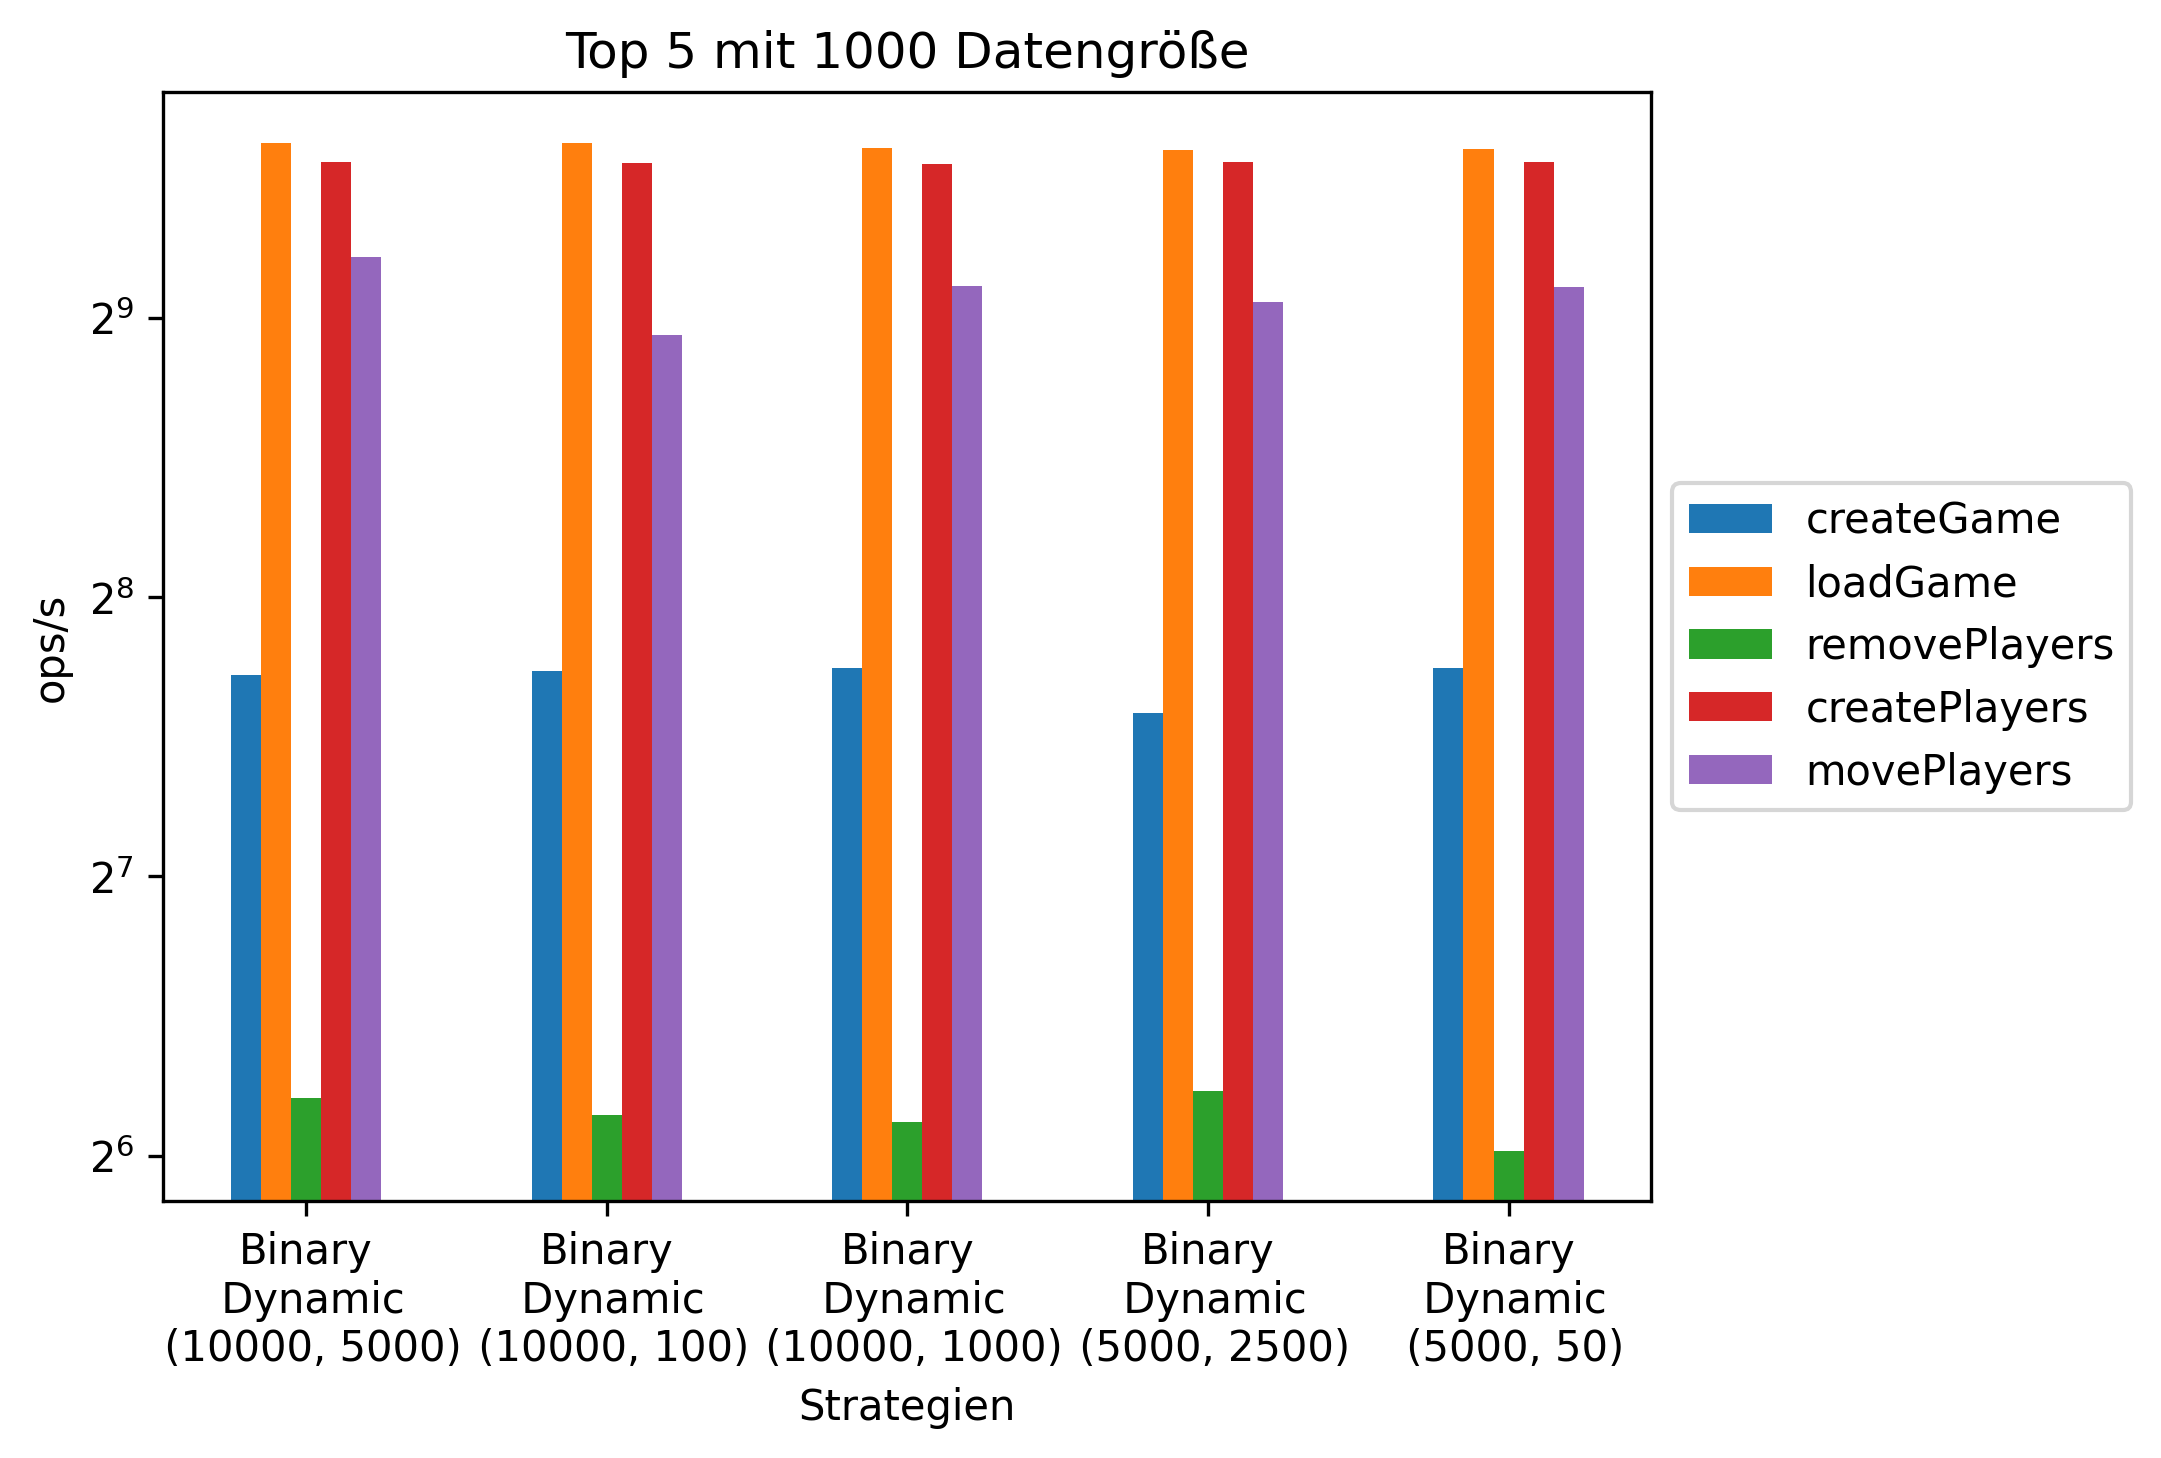
\includegraphics[width=0.7\textwidth]{images/plots/1000.png}
    \caption{Beste Strategien bei einer Datengröße von 1000}
    \label{fig:smallDataCount}
\end{figure}

\begin{figure}[htp]
    \centering
    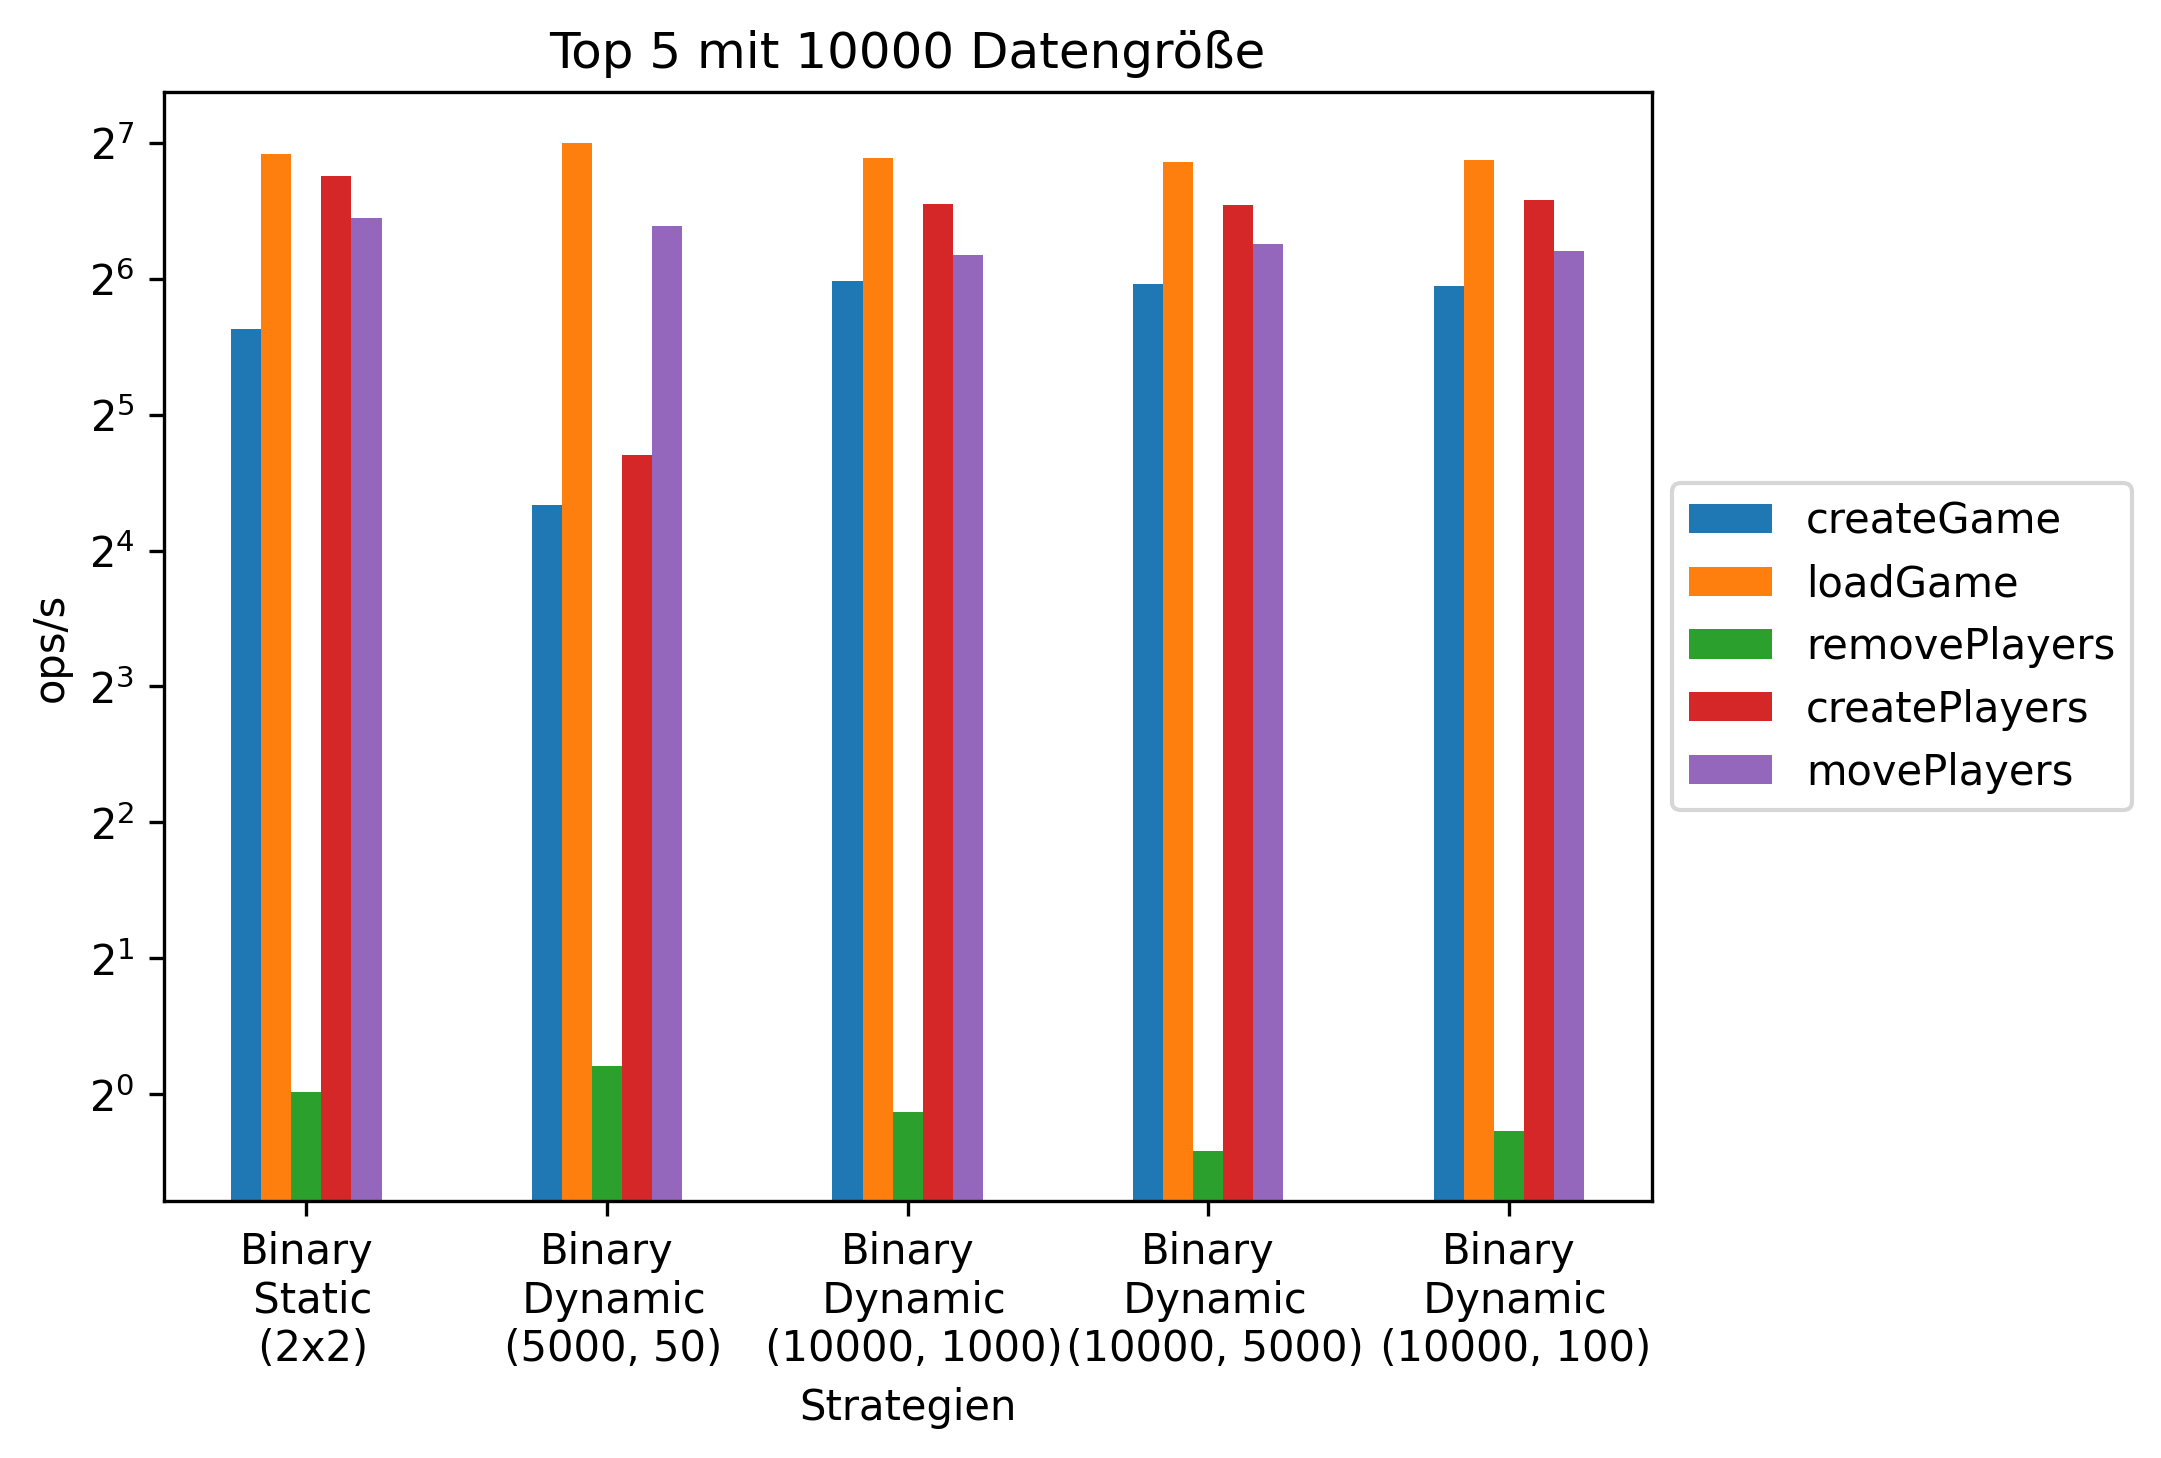
\includegraphics[width=0.7\textwidth]{images/plots/10000.png}
    \caption{Beste Strategien bei einer Datengröße von 10000}
    \label{fig:middleDataCount}
\end{figure}

\begin{figure}[htp]
    \centering
    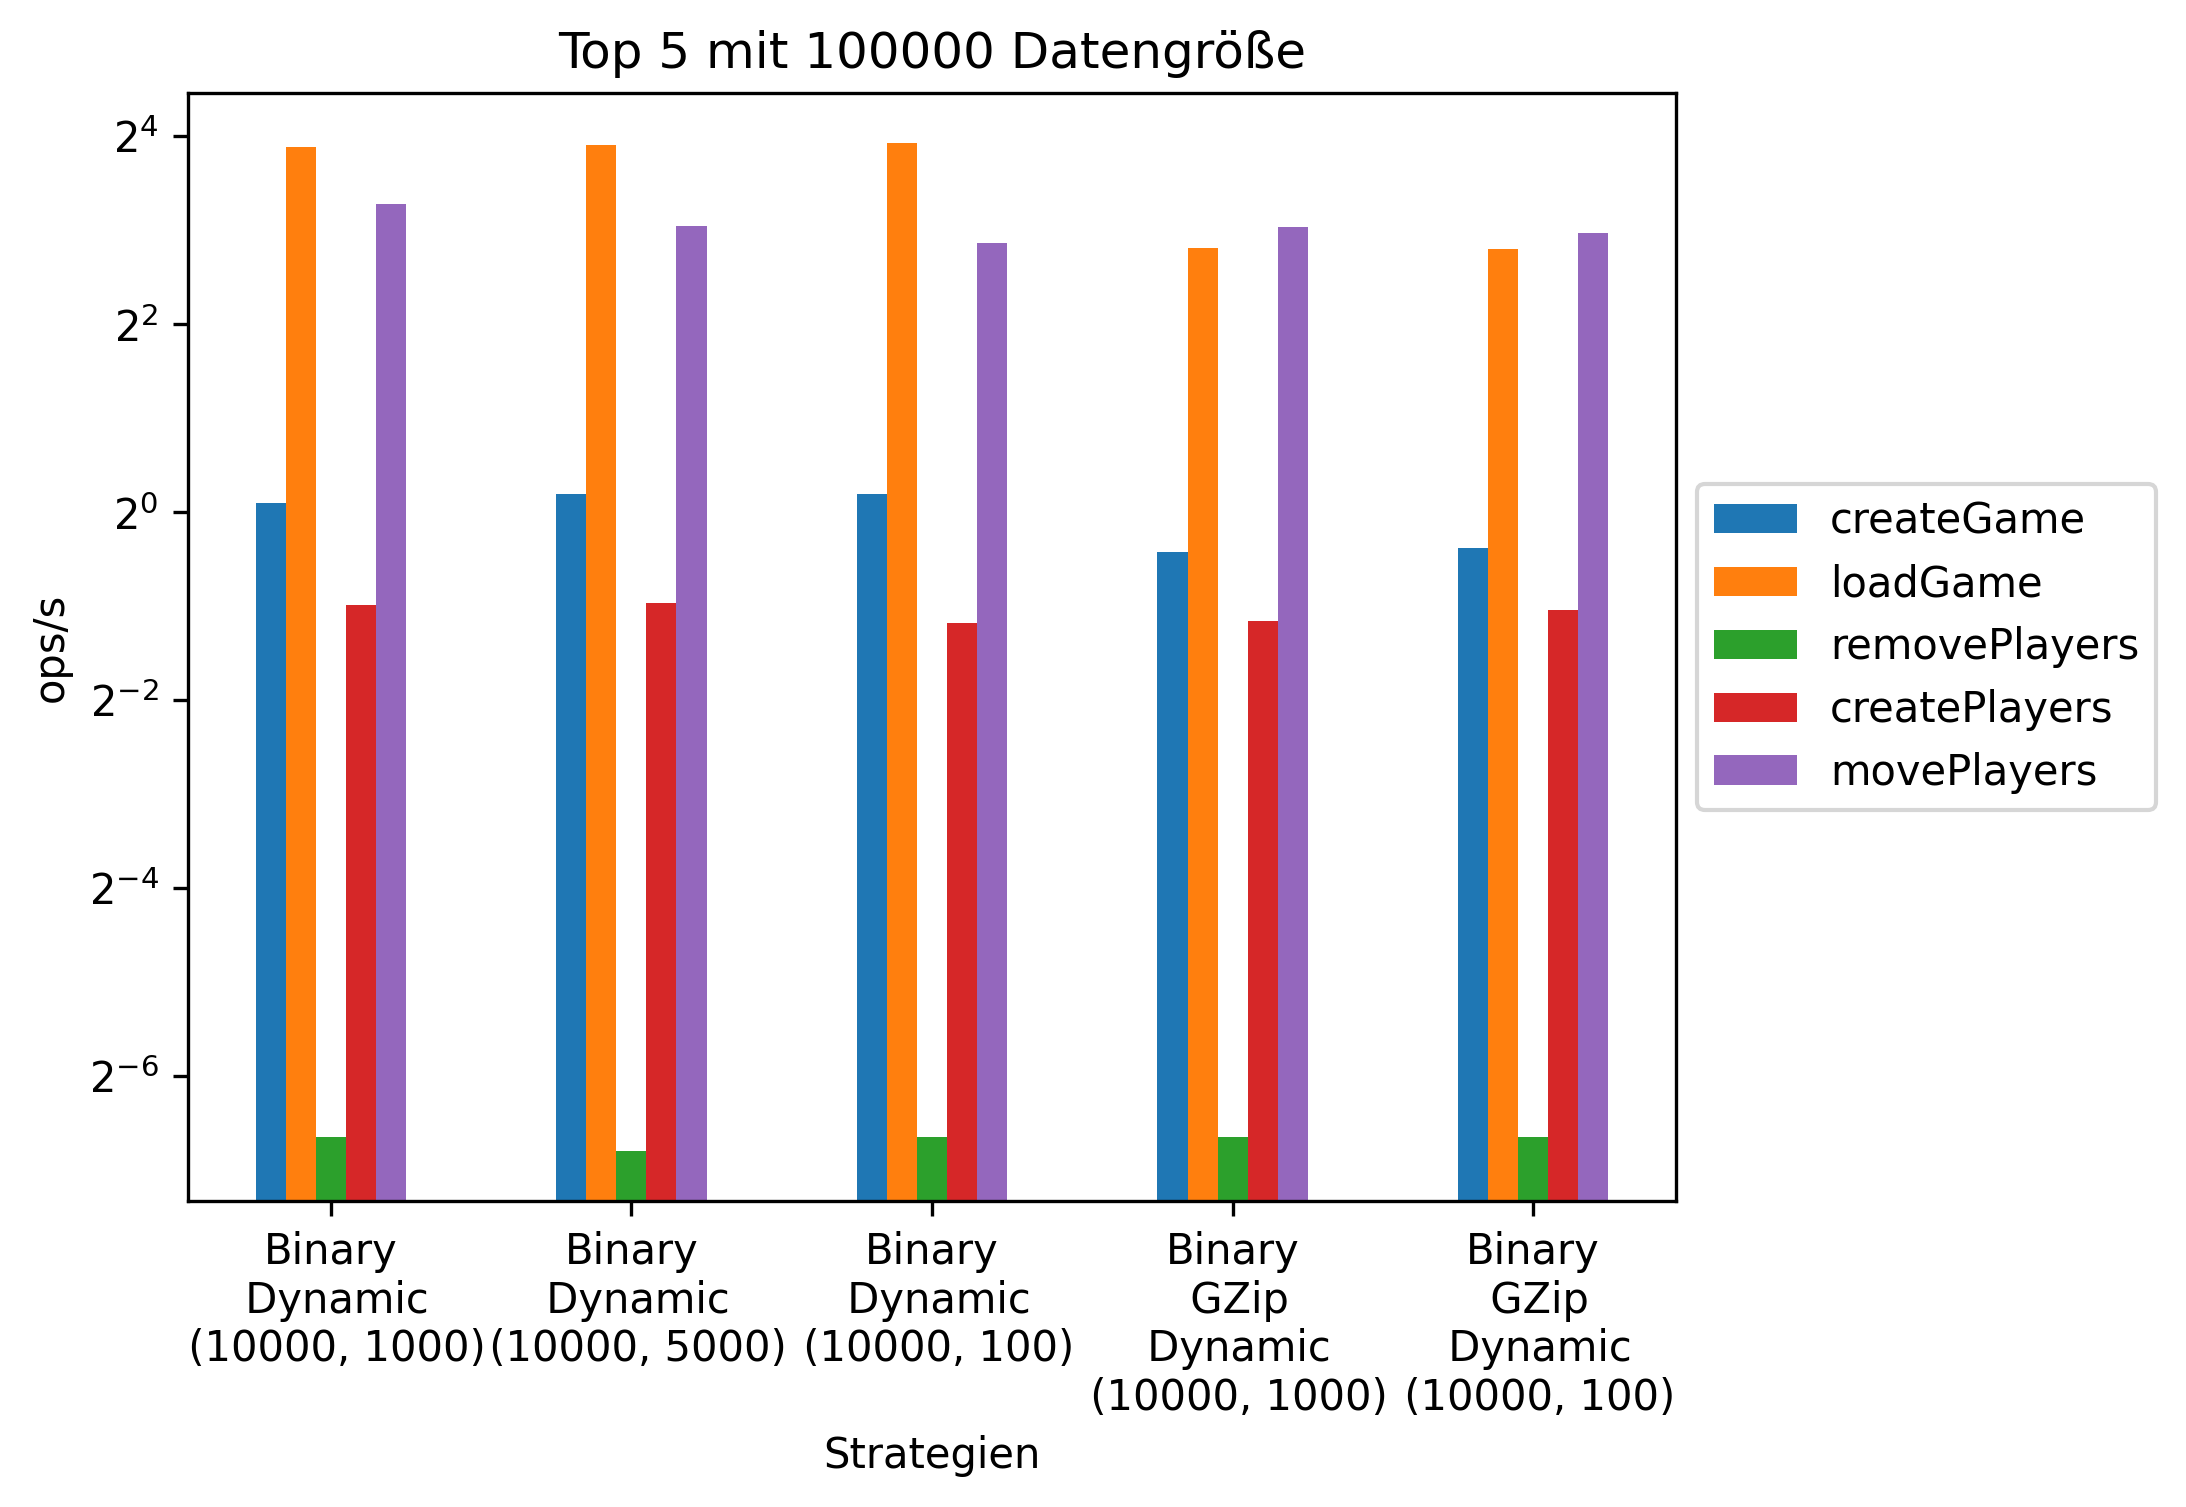
\includegraphics[width=0.7\textwidth]{images/plots/100000.png}
    \caption{Beste Strategien bei einer Daten-Anzahl von 100000}
    \label{fig:bigDataCount}
\end{figure}

\begin{figure}[htp]
    \centering
    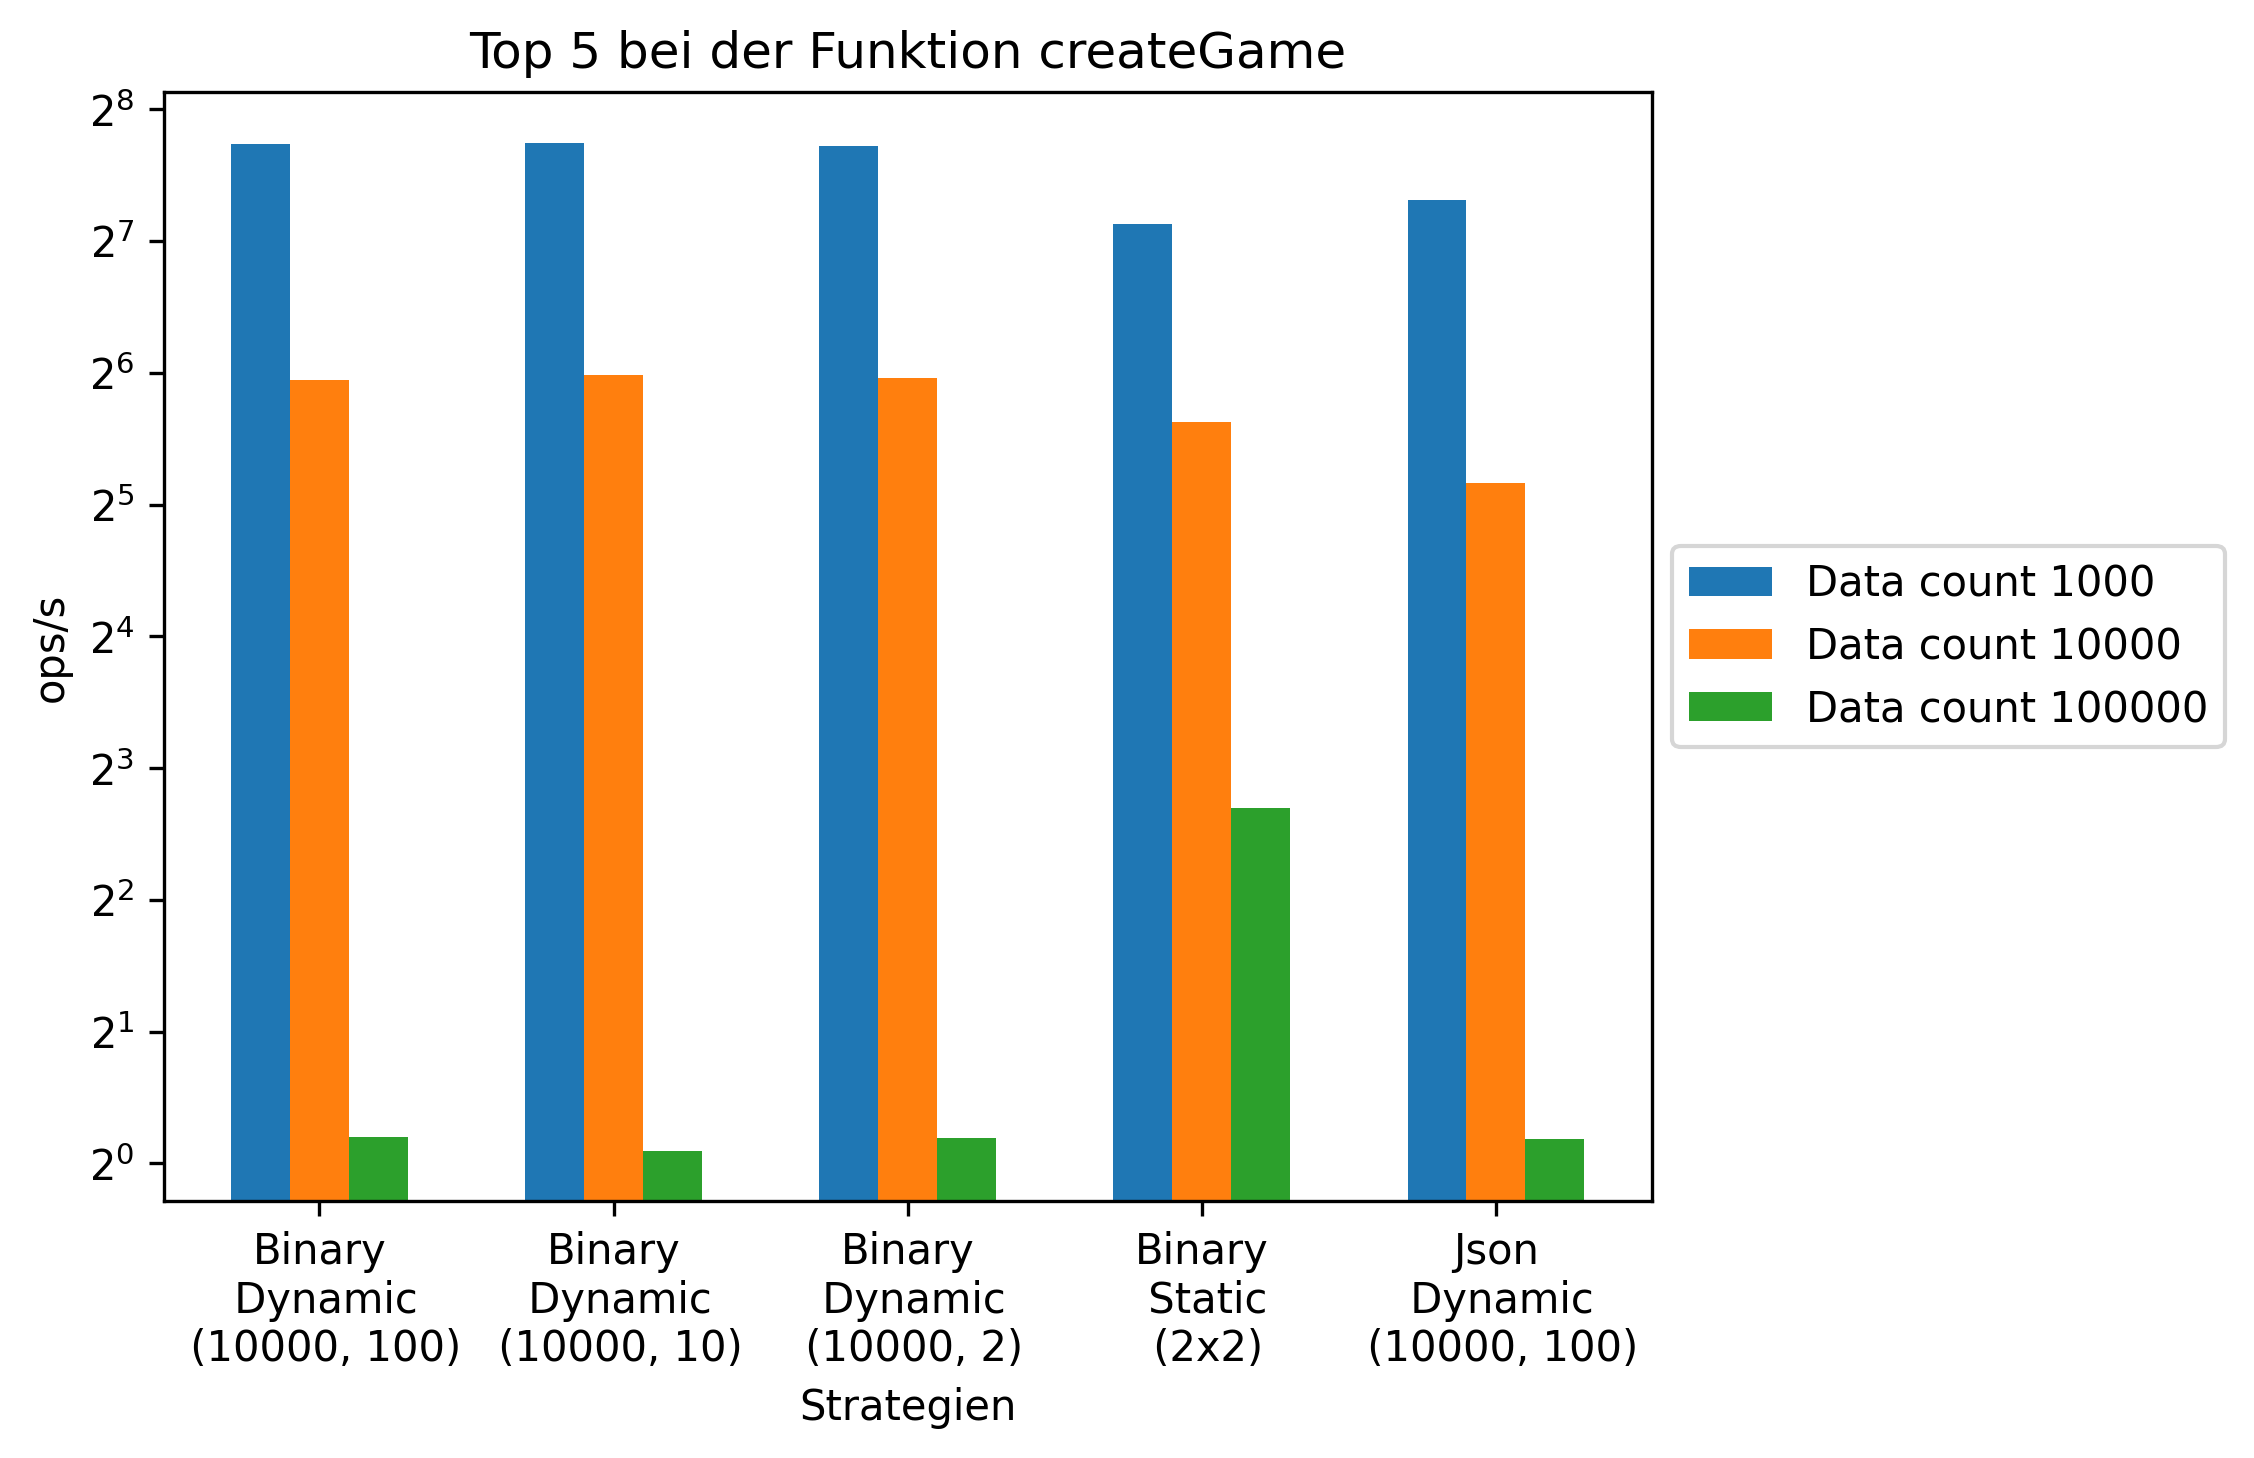
\includegraphics[width=0.7\textwidth]{images/plots/createGame.png}
    \caption{Beste Strategien für die Funktion createGame}
    \label{fig:createGame}
\end{figure}

\begin{figure}[htp]
    \centering
    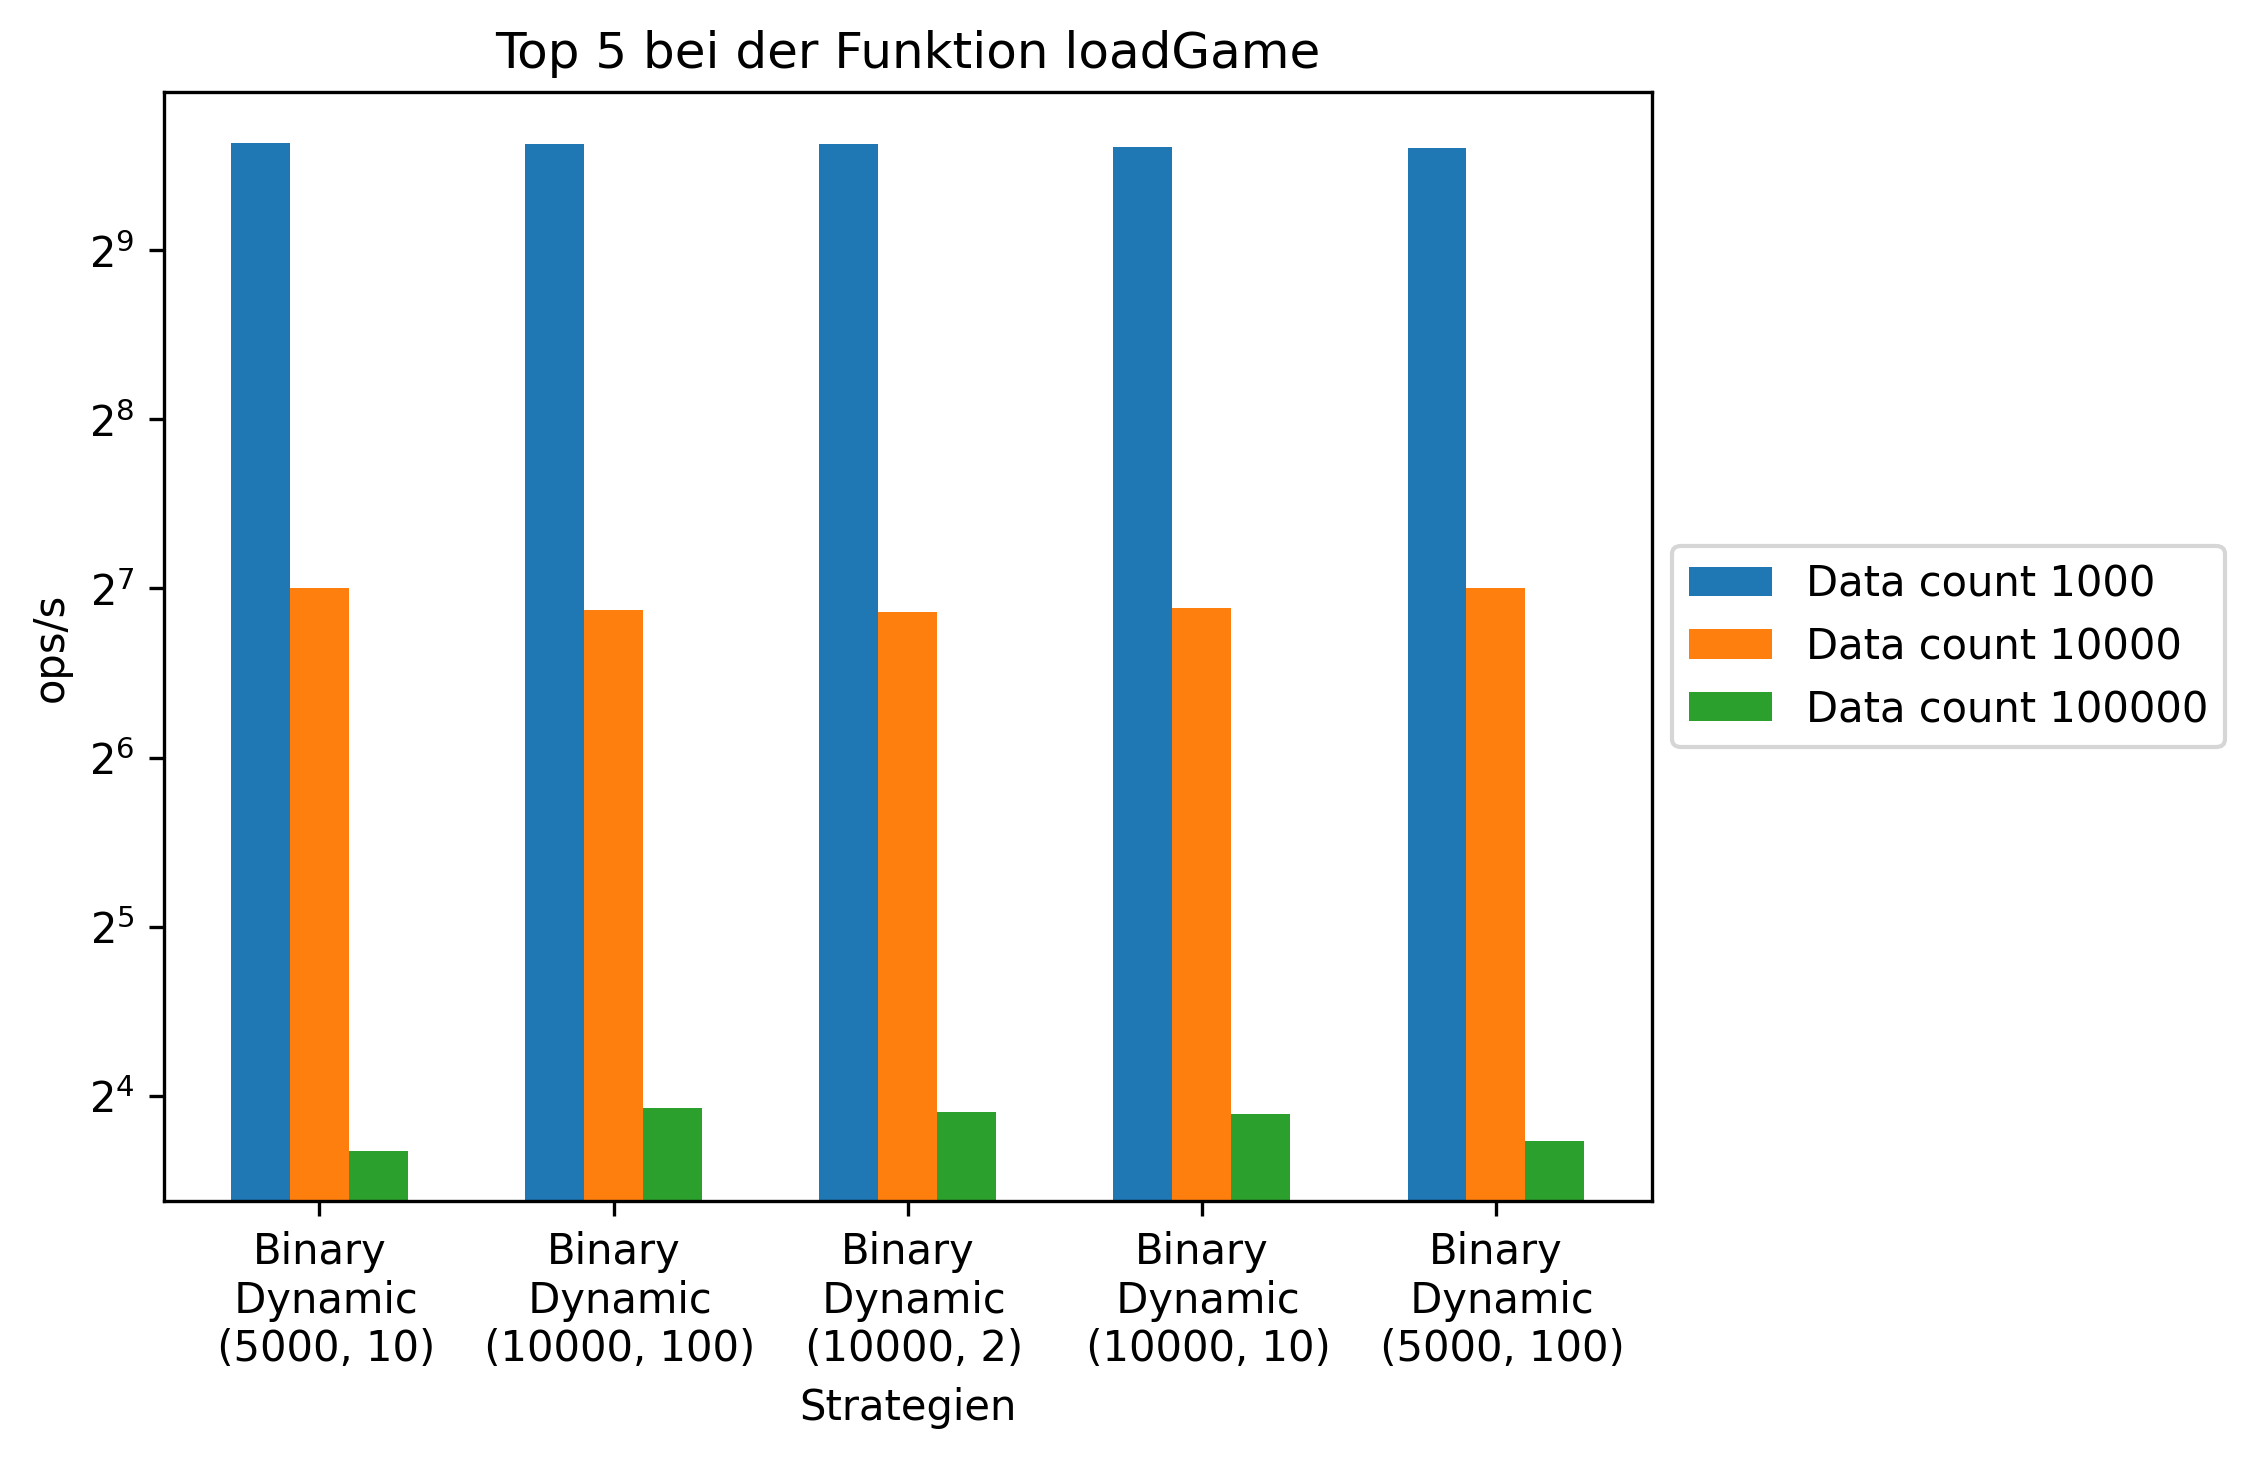
\includegraphics[width=0.7\textwidth]{images/plots/loadGame.png}
    \caption{Beste Strategien für die Funktion loadGame}
    \label{fig:loadGame}
\end{figure}

\begin{figure}[htp]
    \centering
    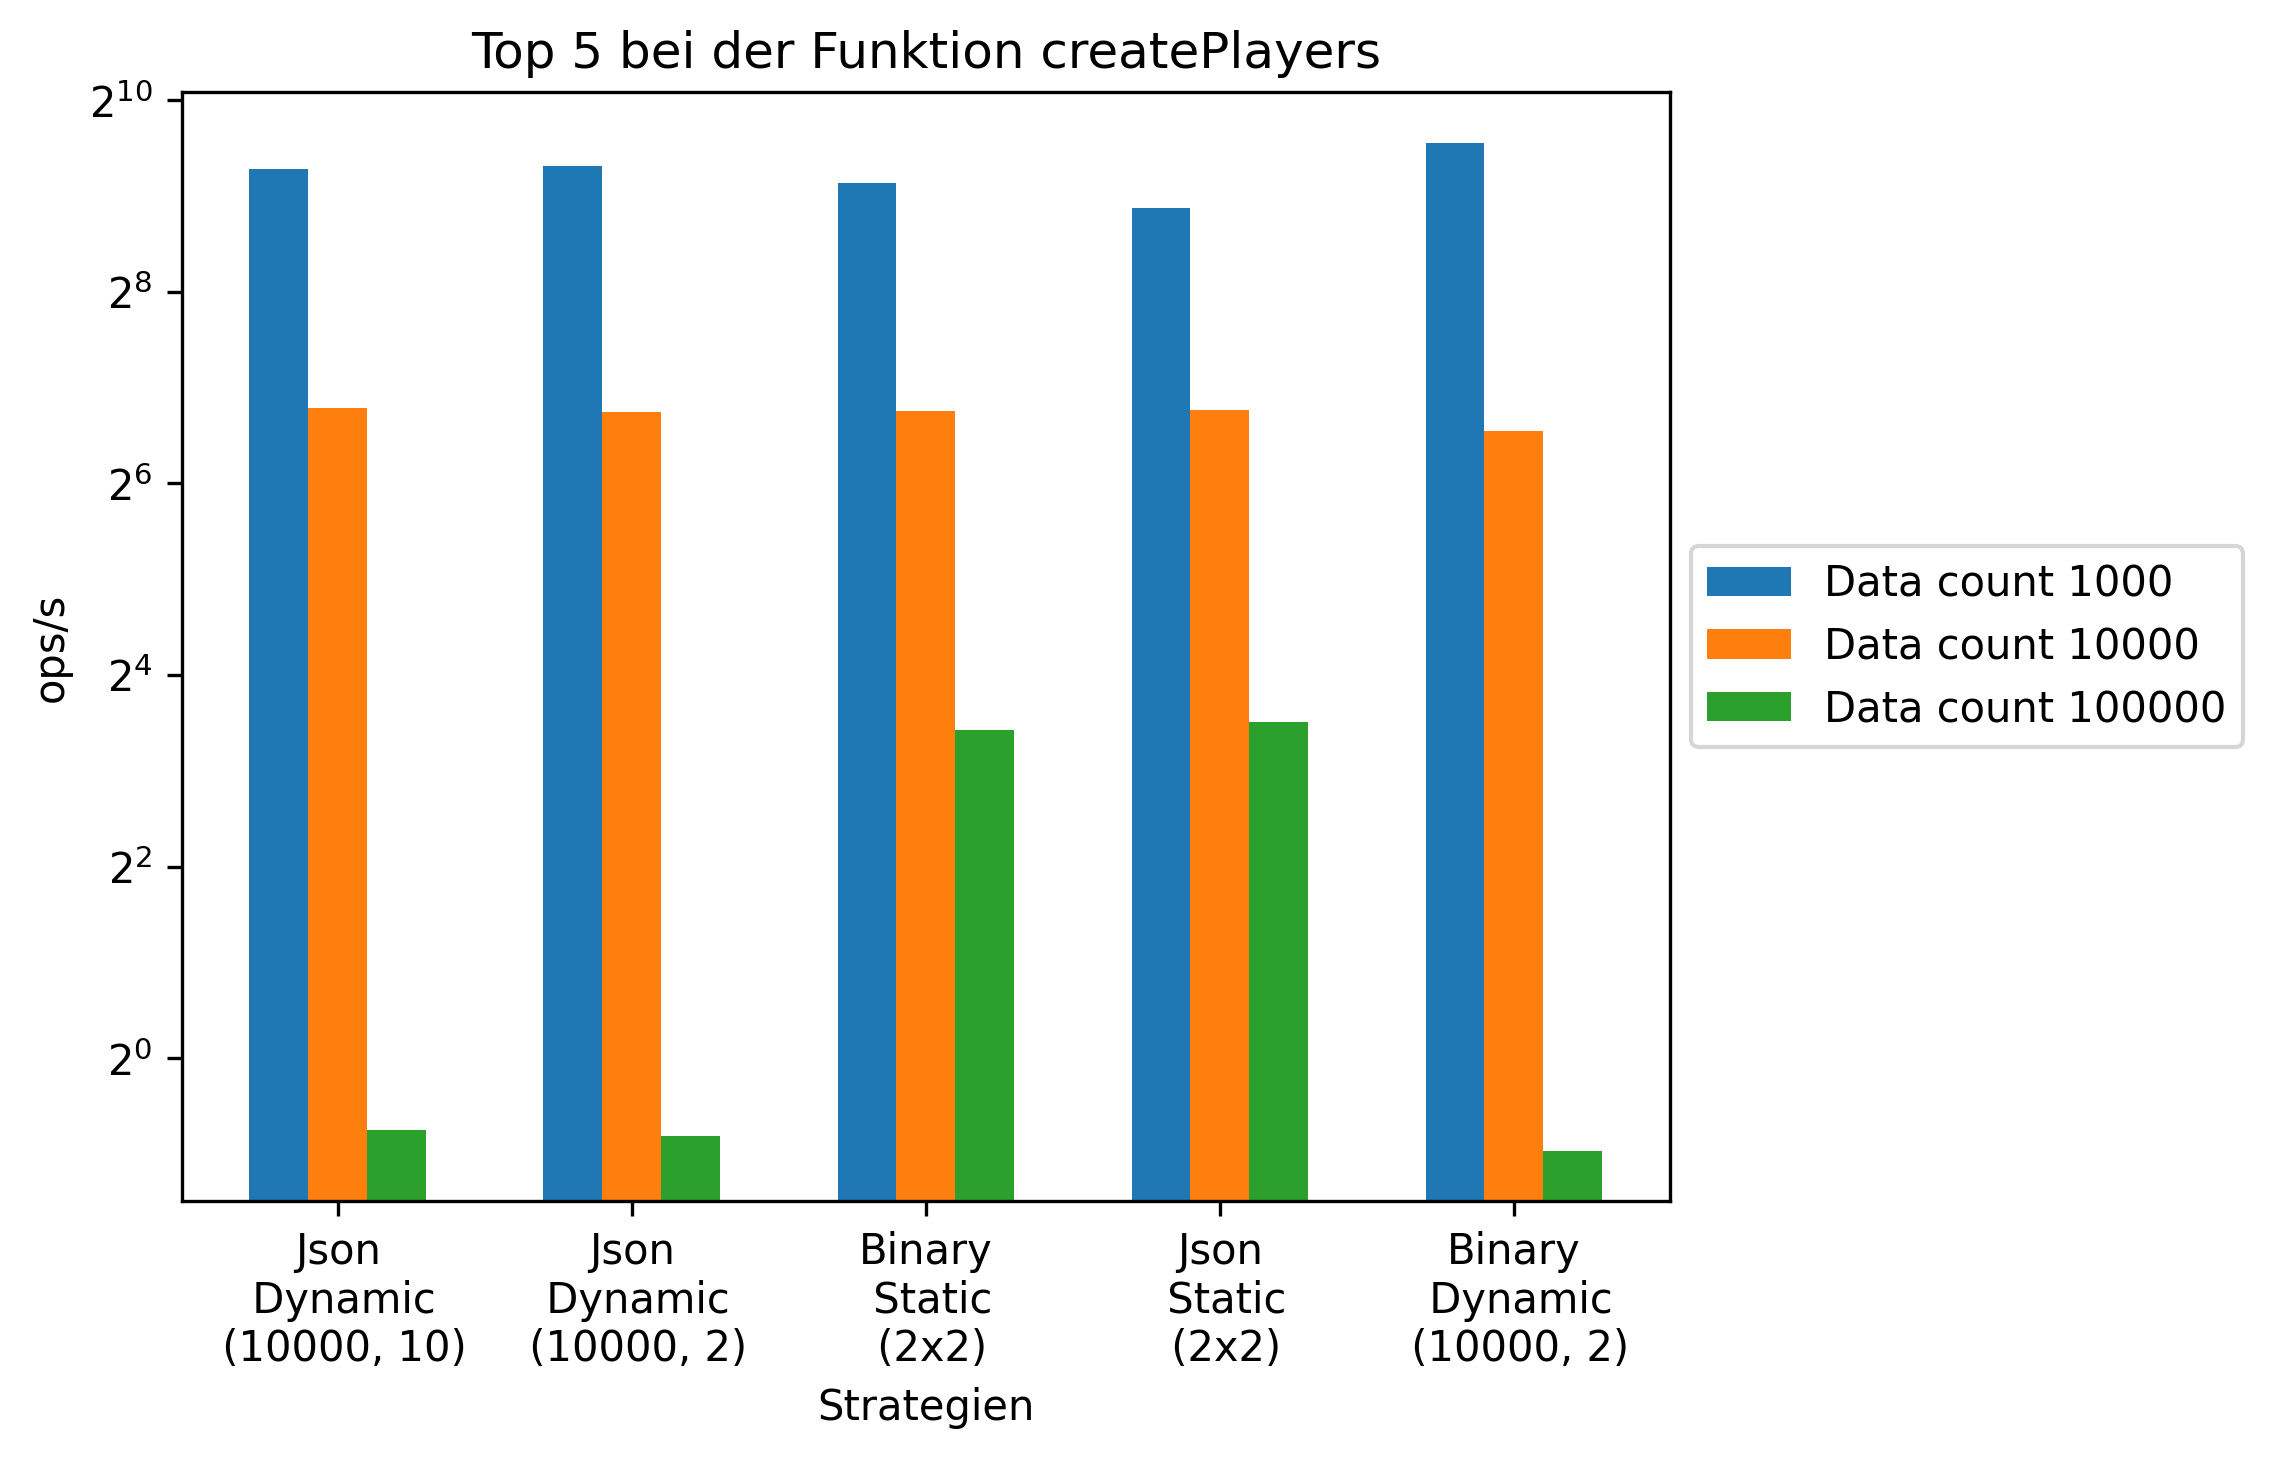
\includegraphics[width=0.7\textwidth]{images/plots/createPlayers.png}
    \caption{Beste Strategien für die Funktion createPlayers}
    \label{fig:createPlayers}
\end{figure}

\begin{figure}[htp]
    \centering
    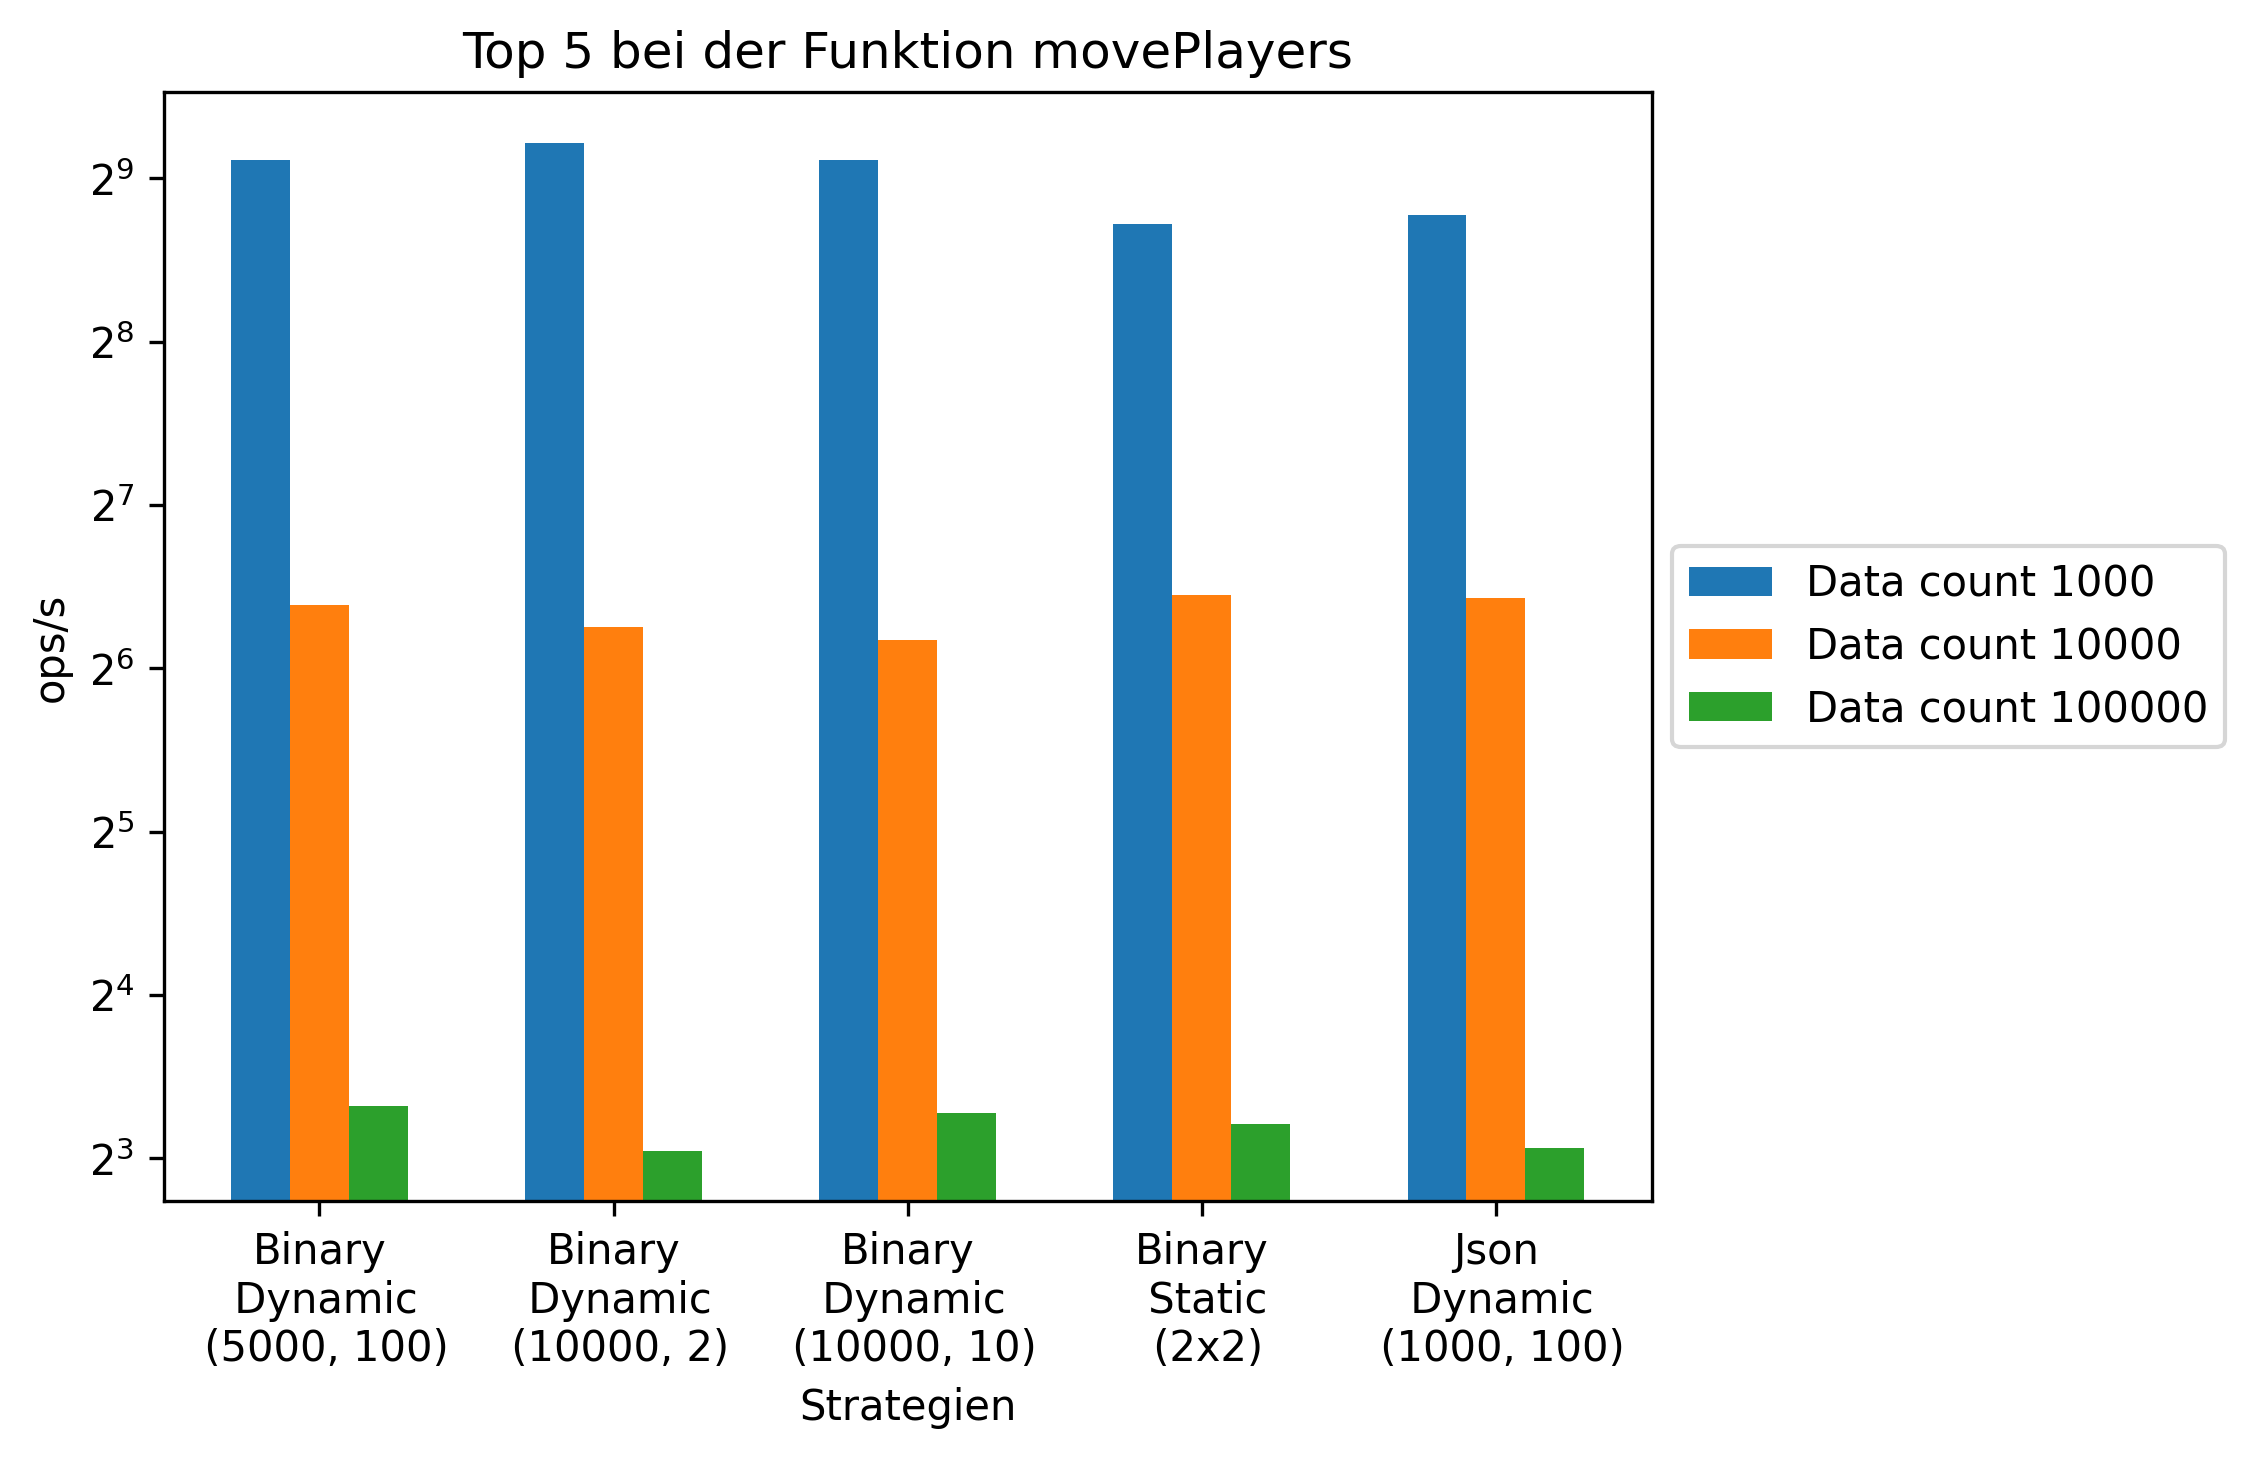
\includegraphics[width=0.7\textwidth]{images/plots/movePlayers.png}
    \caption{Beste Strategien für die Funktion movePlayers}
    \label{fig:movePlayers}
\end{figure}

\begin{figure}[htp]
    \centering
    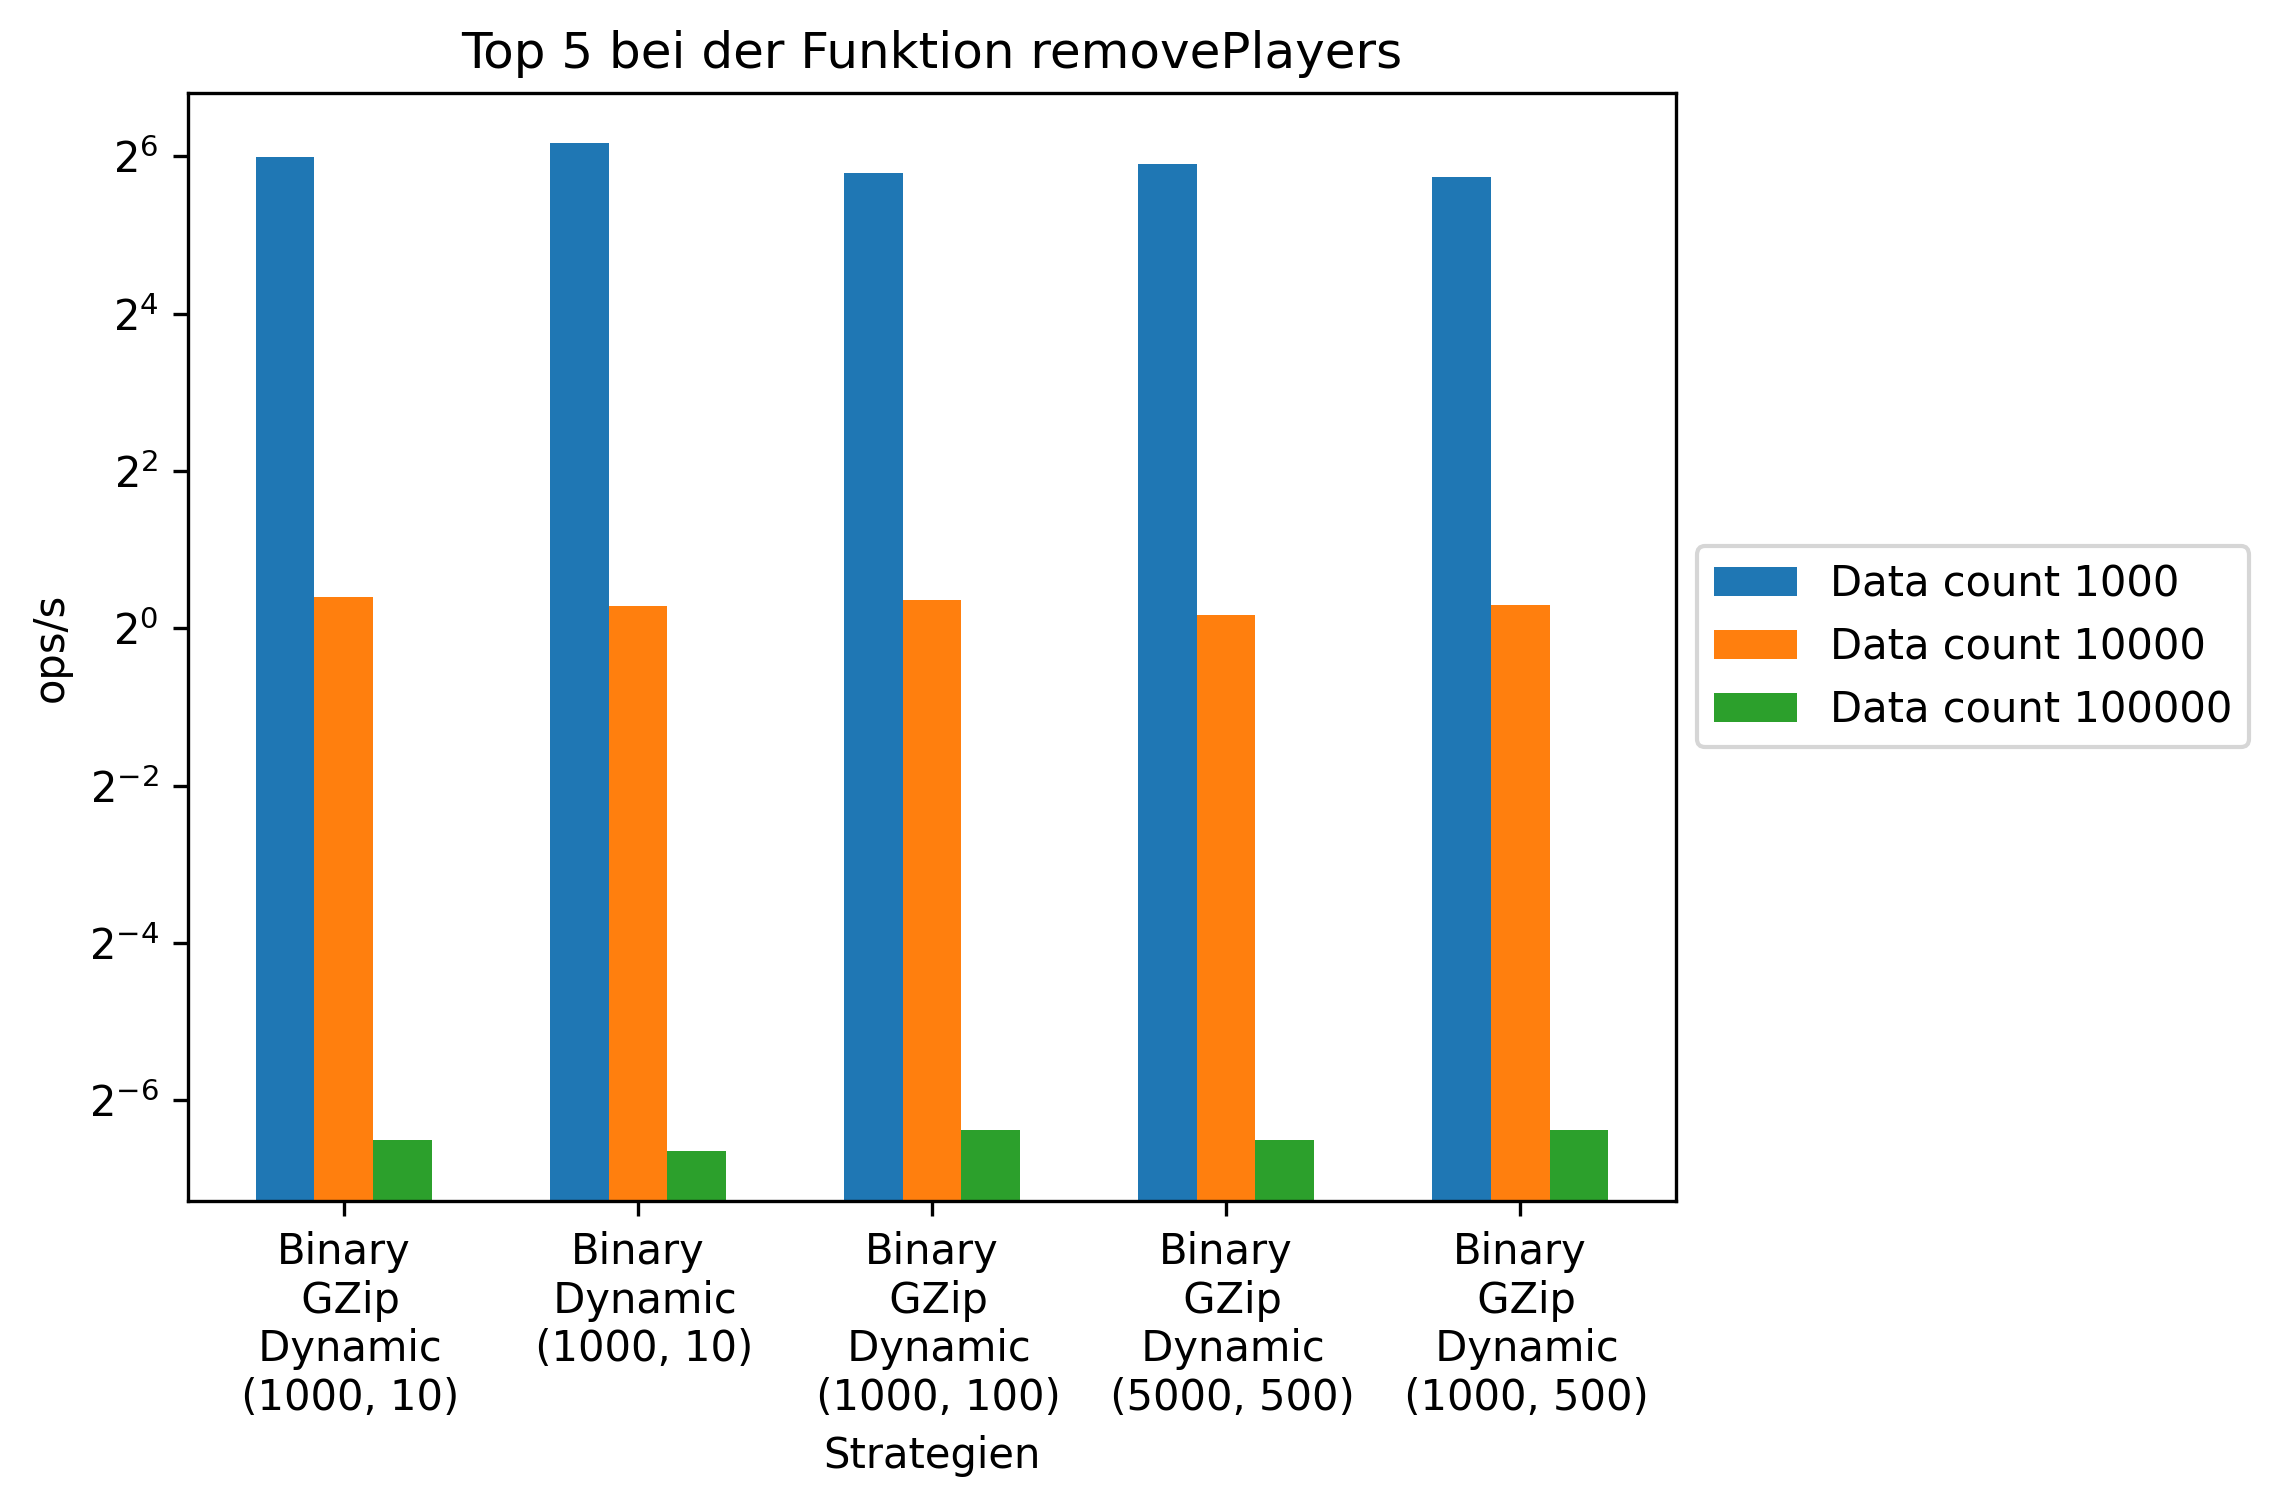
\includegraphics[width=0.7\textwidth]{images/plots/removePlayers.png}
    \caption{Beste Strategien für die Funktion removePlayers}
    \label{fig:removePlayers}
\end{figure}

\begin{figure}[htp]
    \centering
    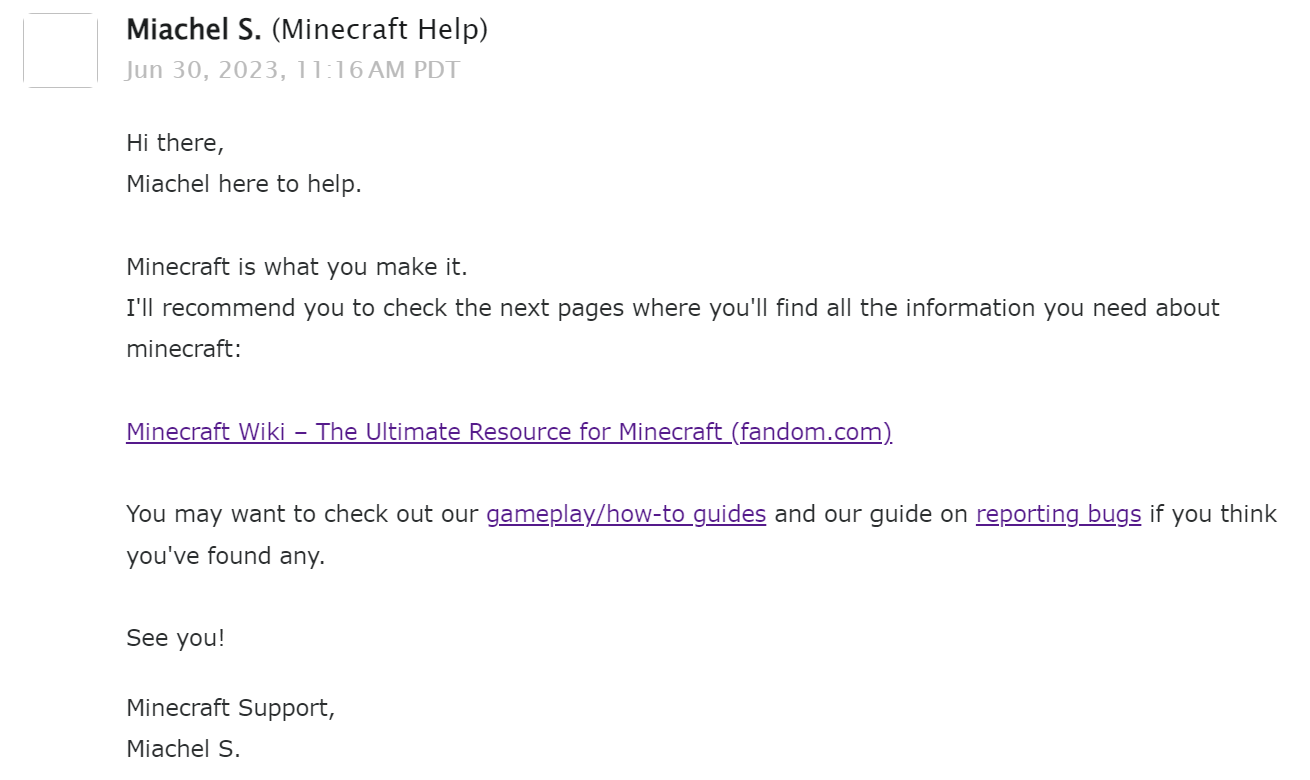
\includegraphics[width=1\textwidth]{images/Minecraft_Email.png}
    \caption{Email von Minecraft zu dem Speicher- und Ladesystem}
    \label{fig:minecraftMail}
\end{figure}

\begin{figure}[htp]
    \centering
    
\includegraphics[width=1\textwidth]{images/Factorio_Email.png}
    \caption{Email von Factorio zu dem Speicher- und Ladesystem}
    \label{fig:factorioMail}
\end{figure}

\end{document}
